\documentclass[]{book}
\usepackage{lmodern}
\usepackage{amssymb,amsmath}
\usepackage{ifxetex,ifluatex}
\usepackage{fixltx2e} % provides \textsubscript
\ifnum 0\ifxetex 1\fi\ifluatex 1\fi=0 % if pdftex
  \usepackage[T1]{fontenc}
  \usepackage[utf8]{inputenc}
\else % if luatex or xelatex
  \ifxetex
    \usepackage{mathspec}
  \else
    \usepackage{fontspec}
  \fi
  \defaultfontfeatures{Ligatures=TeX,Scale=MatchLowercase}
\fi
% use upquote if available, for straight quotes in verbatim environments
\IfFileExists{upquote.sty}{\usepackage{upquote}}{}
% use microtype if available
\IfFileExists{microtype.sty}{%
\usepackage{microtype}
\UseMicrotypeSet[protrusion]{basicmath} % disable protrusion for tt fonts
}{}
\usepackage[margin=1in]{geometry}
\usepackage{hyperref}
\hypersetup{unicode=true,
            pdftitle={Elementary Statistical Modeling for Applied Biostatistics},
            pdfauthor={Jeffrey A. Walker},
            pdfborder={0 0 0},
            breaklinks=true}
\urlstyle{same}  % don't use monospace font for urls
\usepackage{natbib}
\bibliographystyle{apalike}
\usepackage{color}
\usepackage{fancyvrb}
\newcommand{\VerbBar}{|}
\newcommand{\VERB}{\Verb[commandchars=\\\{\}]}
\DefineVerbatimEnvironment{Highlighting}{Verbatim}{commandchars=\\\{\}}
% Add ',fontsize=\small' for more characters per line
\usepackage{framed}
\definecolor{shadecolor}{RGB}{248,248,248}
\newenvironment{Shaded}{\begin{snugshade}}{\end{snugshade}}
\newcommand{\KeywordTok}[1]{\textcolor[rgb]{0.13,0.29,0.53}{\textbf{#1}}}
\newcommand{\DataTypeTok}[1]{\textcolor[rgb]{0.13,0.29,0.53}{#1}}
\newcommand{\DecValTok}[1]{\textcolor[rgb]{0.00,0.00,0.81}{#1}}
\newcommand{\BaseNTok}[1]{\textcolor[rgb]{0.00,0.00,0.81}{#1}}
\newcommand{\FloatTok}[1]{\textcolor[rgb]{0.00,0.00,0.81}{#1}}
\newcommand{\ConstantTok}[1]{\textcolor[rgb]{0.00,0.00,0.00}{#1}}
\newcommand{\CharTok}[1]{\textcolor[rgb]{0.31,0.60,0.02}{#1}}
\newcommand{\SpecialCharTok}[1]{\textcolor[rgb]{0.00,0.00,0.00}{#1}}
\newcommand{\StringTok}[1]{\textcolor[rgb]{0.31,0.60,0.02}{#1}}
\newcommand{\VerbatimStringTok}[1]{\textcolor[rgb]{0.31,0.60,0.02}{#1}}
\newcommand{\SpecialStringTok}[1]{\textcolor[rgb]{0.31,0.60,0.02}{#1}}
\newcommand{\ImportTok}[1]{#1}
\newcommand{\CommentTok}[1]{\textcolor[rgb]{0.56,0.35,0.01}{\textit{#1}}}
\newcommand{\DocumentationTok}[1]{\textcolor[rgb]{0.56,0.35,0.01}{\textbf{\textit{#1}}}}
\newcommand{\AnnotationTok}[1]{\textcolor[rgb]{0.56,0.35,0.01}{\textbf{\textit{#1}}}}
\newcommand{\CommentVarTok}[1]{\textcolor[rgb]{0.56,0.35,0.01}{\textbf{\textit{#1}}}}
\newcommand{\OtherTok}[1]{\textcolor[rgb]{0.56,0.35,0.01}{#1}}
\newcommand{\FunctionTok}[1]{\textcolor[rgb]{0.00,0.00,0.00}{#1}}
\newcommand{\VariableTok}[1]{\textcolor[rgb]{0.00,0.00,0.00}{#1}}
\newcommand{\ControlFlowTok}[1]{\textcolor[rgb]{0.13,0.29,0.53}{\textbf{#1}}}
\newcommand{\OperatorTok}[1]{\textcolor[rgb]{0.81,0.36,0.00}{\textbf{#1}}}
\newcommand{\BuiltInTok}[1]{#1}
\newcommand{\ExtensionTok}[1]{#1}
\newcommand{\PreprocessorTok}[1]{\textcolor[rgb]{0.56,0.35,0.01}{\textit{#1}}}
\newcommand{\AttributeTok}[1]{\textcolor[rgb]{0.77,0.63,0.00}{#1}}
\newcommand{\RegionMarkerTok}[1]{#1}
\newcommand{\InformationTok}[1]{\textcolor[rgb]{0.56,0.35,0.01}{\textbf{\textit{#1}}}}
\newcommand{\WarningTok}[1]{\textcolor[rgb]{0.56,0.35,0.01}{\textbf{\textit{#1}}}}
\newcommand{\AlertTok}[1]{\textcolor[rgb]{0.94,0.16,0.16}{#1}}
\newcommand{\ErrorTok}[1]{\textcolor[rgb]{0.64,0.00,0.00}{\textbf{#1}}}
\newcommand{\NormalTok}[1]{#1}
\usepackage{longtable,booktabs}
\usepackage{graphicx,grffile}
\makeatletter
\def\maxwidth{\ifdim\Gin@nat@width>\linewidth\linewidth\else\Gin@nat@width\fi}
\def\maxheight{\ifdim\Gin@nat@height>\textheight\textheight\else\Gin@nat@height\fi}
\makeatother
% Scale images if necessary, so that they will not overflow the page
% margins by default, and it is still possible to overwrite the defaults
% using explicit options in \includegraphics[width, height, ...]{}
\setkeys{Gin}{width=\maxwidth,height=\maxheight,keepaspectratio}
\IfFileExists{parskip.sty}{%
\usepackage{parskip}
}{% else
\setlength{\parindent}{0pt}
\setlength{\parskip}{6pt plus 2pt minus 1pt}
}
\setlength{\emergencystretch}{3em}  % prevent overfull lines
\providecommand{\tightlist}{%
  \setlength{\itemsep}{0pt}\setlength{\parskip}{0pt}}
\setcounter{secnumdepth}{5}
% Redefines (sub)paragraphs to behave more like sections
\ifx\paragraph\undefined\else
\let\oldparagraph\paragraph
\renewcommand{\paragraph}[1]{\oldparagraph{#1}\mbox{}}
\fi
\ifx\subparagraph\undefined\else
\let\oldsubparagraph\subparagraph
\renewcommand{\subparagraph}[1]{\oldsubparagraph{#1}\mbox{}}
\fi

%%% Use protect on footnotes to avoid problems with footnotes in titles
\let\rmarkdownfootnote\footnote%
\def\footnote{\protect\rmarkdownfootnote}

%%% Change title format to be more compact
\usepackage{titling}

% Create subtitle command for use in maketitle
\newcommand{\subtitle}[1]{
  \posttitle{
    \begin{center}\large#1\end{center}
    }
}

\setlength{\droptitle}{-2em}
  \title{Elementary Statistical Modeling for Applied Biostatistics}
  \pretitle{\vspace{\droptitle}\centering\huge}
  \posttitle{\par}
  \author{Jeffrey A. Walker}
  \preauthor{\centering\large\emph}
  \postauthor{\par}
  \predate{\centering\large\emph}
  \postdate{\par}
  \date{2018-10-24}

\usepackage{booktabs}
\usepackage{amsthm}
\makeatletter
\def\thm@space@setup{%
  \thm@preskip=8pt plus 2pt minus 4pt
  \thm@postskip=\thm@preskip
}
\makeatother

\usepackage{amsthm}
\newtheorem{theorem}{Theorem}[chapter]
\newtheorem{lemma}{Lemma}[chapter]
\theoremstyle{definition}
\newtheorem{definition}{Definition}[chapter]
\newtheorem{corollary}{Corollary}[chapter]
\newtheorem{proposition}{Proposition}[chapter]
\theoremstyle{definition}
\newtheorem{example}{Example}[chapter]
\theoremstyle{definition}
\newtheorem{exercise}{Exercise}[chapter]
\theoremstyle{remark}
\newtheorem*{remark}{Remark}
\newtheorem*{solution}{Solution}
\begin{document}
\maketitle

{
\setcounter{tocdepth}{1}
\tableofcontents
}
\chapter{Statistical Modeling}\label{statistical-modeling}

\emph{More cynically, one could also well ask ``Why has medicine not
adopted frequentist inference, even though everyone presents P-values
and hypothesis tests?'' My answer is: Because frequentist inference,
like Bayesian inference, is not taught. Instead everyone gets taught a
misleading pseudo-frequentism: a set of rituals and misinterpretations
caricaturing frequentist inference, leading to all kinds of
misunderstandings.} -- Sander Greenland

We use statistics to learn from data with uncertainty. Traditional
introductory textbooks in biostatistics implicitly or explicitly train
students and researchers to ``discover by p-value'' using hypothesis
tests (appendix xxx). Over the course of many chapters, the student is
trained to use something like a dichotomous key to choose the correct
``test'' for the data at hand, compute a test statistic for their data,
compute a \(p\)-value based on the test statistic, and compares the
\emph{p}-value to 0.05. Textbooks typically give very little guidance
about what can be concluded if \(p < 0.05\) or if \(p > 0.05\), but many
researchers conclude (incorrectly) they have ``discovered'' something if
\(p < 0.05\) but found ``no effect'' if \(p > 0.05\).

Researchers learn almost nothing useful from a hypothesis test. True, a
\(p\)-value is evidence against the null, and thus, a tool to dampen our
tendency to being fooled by randomness. But if we are investigating the
effects of an increasingly acidified ocean on coral growth, \(p=0.002\)
may be evidence of an effect of the experimental intervention, but, from
everything we know about pH and cell biology, it would be absurd to
conclude from any data that pH does not affect growth. Instead, we want
to know the magnitude of the effect and our uncertainty in estimating
this magnitude. We can use this magnitude and uncertainty to make
predictions about the future of coral reefs, under different scenarios
of ocean acidification. We can use the estimated effects and uncertainty
to model the consquences of the effects of acidification on coral growth
on fish production or carbon cycling.

The ``discovery by p-value'' strategy, or Null-Hypothesis Significance
Testing (NHST), has been criticized by statisticians for many, many
decades. Nevertheless, introductory biostatistics textbooks written by
both biologists and statisticians continue to organize textbooks around
a collection of hypothesis tests, with little emphasis on estimation and
uncertainty.

\section{Statistical modeling with linear
models}\label{statistical-modeling-with-linear-models}

This book is an introduction to the analysis of biological data using a
statistical modeling approach. As an introduction, the focus will be
linear models and extensions of the linear models including linear mixed
models and generalized linear models. Here, I refer to all of these as
``linear models'' because all are a function of a linear predictor.
Linear models are the engine behind many hypothesis tests but the
emphasis in statistical modeling is estimation and uncertainty instead
of test statistics and \(p\)-values. A modeling view of statistics is
also more coherent than a dichotomous key strategy.

\begin{figure}
\centering
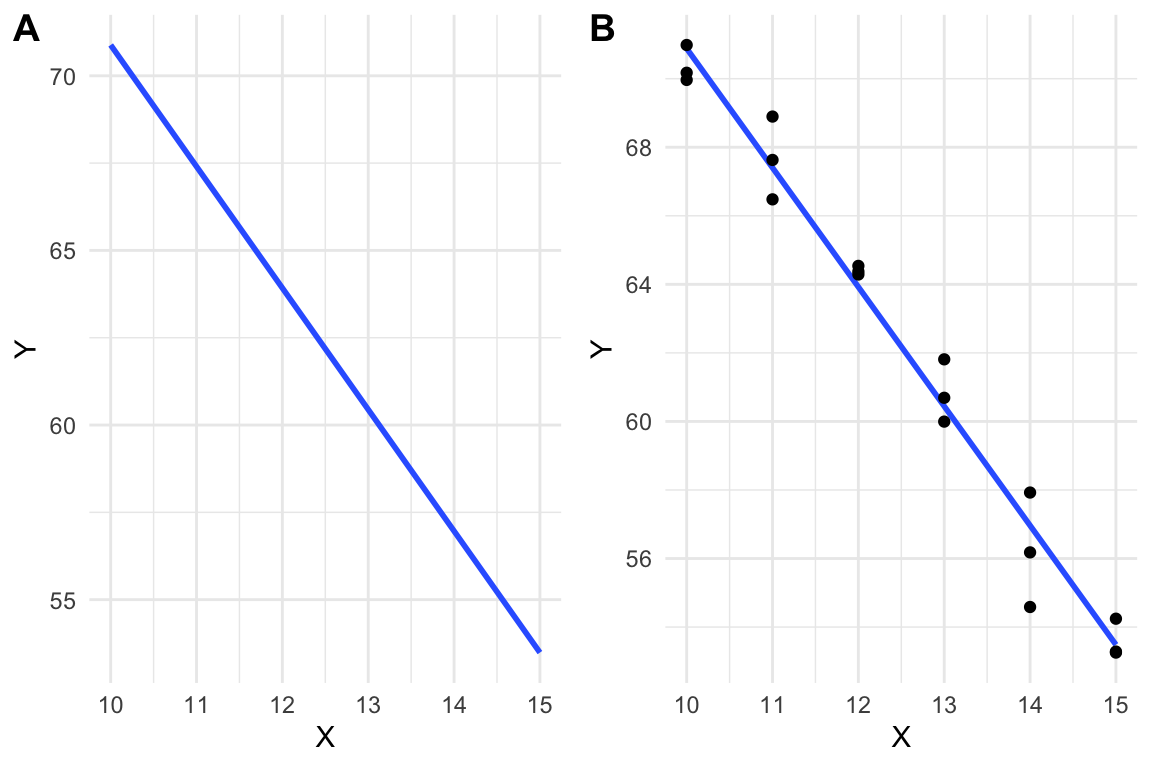
\includegraphics{Walker-elementary-statistical-modeling-draft_files/figure-latex/line-1.pdf}
\caption{\label{fig:line}A line vs.~a linear model. (A) the line \$y=-3.48X
+ 105.7 is drawn. (B) A linear model fit to the data. The model
coefficients are numerically equal to the slope and intercept of the
line in A.}
\end{figure}

All students are familiar with the idea of a linear model from learning
the equation of a line, which is

\begin{equation}
Y = mX + b
\label{eq:line}
\end{equation}

where \(m\) is the slope of the line and \(b\) is the \(Y\)-intercept.
It is useful to think of equation \eqref{eq:line} as a function that maps
values of \(X\) to values of \(Y\). Using this function, if we input
some value of \(X\), we always get the same value of Y as the output.

A linear model is a function, like that in equation \eqref{eq:line}, that
is fit to a set of data, often to model a process that generated the
data or something like the data. The line in Figure \ref{fig:line}A is
just that, a line, but the line in Figure \ref{fig:line}B is a model of
the data in Figure \ref{fig:line}B. The basic structure of a linear
model is

\begin{equation}
Y = \beta_0 + \beta_1 X + \varepsilon
\label{eq:lm}
\end{equation}

A linear model has two parts: the ``linear predictor''
(\(Y = \beta_0 + \beta_1 X\)) and the ``error'' (\(\varepsilon\)). The
linear predictor part looks like the equation for a line except that
I've used \(\beta_0\) for the intercept and \(\beta_1\) for the slope
and I've put the intercept term first. This re-labeling and
re-arrangement make the notation for a linear model more flexible for
more complicated linear models. For example
\(Y = \beta_0 + \beta_1 X_1 + \beta_2 X_2 + \varepsilon\) is a model
where \(Y\) is a function of two \(X\) variables.

As with the equation for a line, the linear predictor part of a linear
model is a function that maps a value of \(X\) to a specific value of
\(Y\). This mapped value is the \textbf{expected value} given a specific
input value of \(X\). This is often written as \(\mathrm{E}[Y|X]\). The
error part of a linear model is a random variable that adds some random
value to this expected value. Nothing about the model part of a linear
model can predict its value.

The inputs to a linear model (the \(X\) variables) have many names
including ``independent variables,'' ``predictor variables,'',
``explanatory variables,'' ``treatment variables,'' and ``covariates''.
The output of a linear model (the \(Y\) variable or variables if the
model is multivariate) is the ``dependent variable,'' ``response,'' or
``outcome.'' The \(\beta\) in the linear model are model
\textbf{parameters} There can be additional parameters in more
sophisticated models. The coefficients of the \(X\) in a linear model
(\(\beta_1\) in model \eqref{eq:lm}) are often called ``the effects'' (so
\(\beta_1\) is the effect of \(X_1\)).

Although a linear model is a model of a data-generating process, linear
models are not typically used to actually generate any data. Instead,
when we use a linear model to understand something about a real dataset,
we think of our data as one realization of a process that generates data
like ours. A linear model is a model of that process. That said, it is
incredibly useful to use linear models to create fake datasets for at
least two reasons: to probe our understanding of statistical modeling
generally and, more specifically, to check that a model actually creates
data like that in the real dataset that we are analyzing.

\subsection{Linear models are used for prediction, explanation, and
description}\label{linear-models-are-used-for-prediction-explanation-and-description}

Researchers typically use linear models to understand relationships
between one or more \(Y\) variables and one or more \(X\) variables.
These relationships include

\begin{enumerate}
\def\labelenumi{\arabic{enumi}.}
\item
  Descriptive modeling. Sometimes a researcher merely wants to describe
  the relationship between \(Y\) and a set of \(X\) variables, perhaps
  to discover patterns. For example, the arrival of a spring migrant
  bird (\(Y\)) as a function of sex (\(X_1\)) and age (\(X_2\)) might
  show that males and younger individuals arrive earlier. Importantly,
  if another \(X\) variable is added to the model (or one dropped), the
  coefficients, and therefore, the precise description, will change.
  That is, the interpretation of a coefficient as a descriptor is
  \emph{conditional} on the other covariates (\(X\) variables) in the
  model. In a descriptive model, there is no implication of causal
  effects and the goal is not prediction. Nevertheless, it is very hard
  for humans to discuss a descriptive model without using causal
  language, which probably means that it is hard for us to think of
  these models as \emph{mere description}. Like natural history,
  descriptive models are useful as patterns in want of an explanation,
  using more explicit causal models including experiments.
\item
  Predictive modeling. Predictive modeling is very common in applied
  research. For example, fisheries researchers might model the
  relationship between population density and habitat variables to
  predict which subset of ponds in a region are most suitable for brook
  trout (\emph{Salvelinus fontinalis}) reintroduction. The goal is to
  build a model with minimal prediction error, which is the error
  between predicted and actual values for a future sample. In predictive
  modeling, the \(X\) (``predictor'') variables are largely instrumental
  -- how these are related to \(Y\) is not a goal of the modeling,
  although sometimes an investigator may be interested in the relative
  importance among the \(X\) for predicting \(Y\) (for example,
  collecting the data may be time consuming, or expensive, or
  enviromentally destructive, so know which subset of \(X\) are most
  important for predicting \(Y\) is a useful strategy).
\item
  Explanatory (causal) modeling. Very often, researchers are explicitly
  interested in \emph{how} the \(X\) variables are causally related to
  \(Y\). The fisheries researchers that want to reintroduce trout may
  want to develop and manage a set of ponds to maintain healthy trout
  populations. This active management requires intervention to change
  habitat traits in a direction, and with a magnitude, to cause the
  desired response. This model is predictive -- a specific change in
  \(X\) predicts a specific response in \(Y\) -- because the
  coefficients of the model provide knowledge on how the system
  functions -- how changes in the inputs \emph{cause} change in the
  output. Causal interpretation of model coefficients requires a set of
  strong assumptions about the \(X\) variables in the model. These
  assumptions are typically met in \textbf{experimental designs} but not
  \textbf{observational designs}.
\end{enumerate}

With observational designs, biologists are often not very explicit about
which of these is the goal of the modeling and use a combination of
descriptive, predictive, and causal language to describe and discuss
results. Many papers read as if the researchers intend explanatory
inference but because of norms within the biology community, mask this
intention with ``predictive'' language. Here, I advocate embracing
explicit, explanatory modeling by being very transparent about the
model's goal and assumptions.

\section{Model fitting}\label{model-fitting}

In order to use a linear model to describe, predict, or explain, we need
to fit a model to data in order to estimate the parameters. If we fit
model \eqref{eq:conditional-expectation} to some data, the estimated
parameters are the coefficients (\(b_0\) and \(b_1\)) of the fit model

\begin{equation}
\mathrm{E}[Y|X] = b_0 + b_1 X
\label{eq:conditional-expectation}
\end{equation}

The left-hand side of equation \eqref{eq:conditional-expectation} is the
\textbf{conditional expectation} and is read as ``the expectation of Y
given X'' or ``the expected value of Y given X''. Throughout this book,
I use the greek \(\beta\) to refer to a theoretical, data-generating
parameter and the roman ``b'' to refer its estimate.

The goal of descriptive and explanatory modeling is the estimate of the
coefficients of the \(X\) variables and their uncertainty. The goal of
predictive modeling is the estimate of predicted values, and their
uncertainty, given specific values of \(X\). These predicted values are
the conditional expectations.

\begin{figure}
\centering
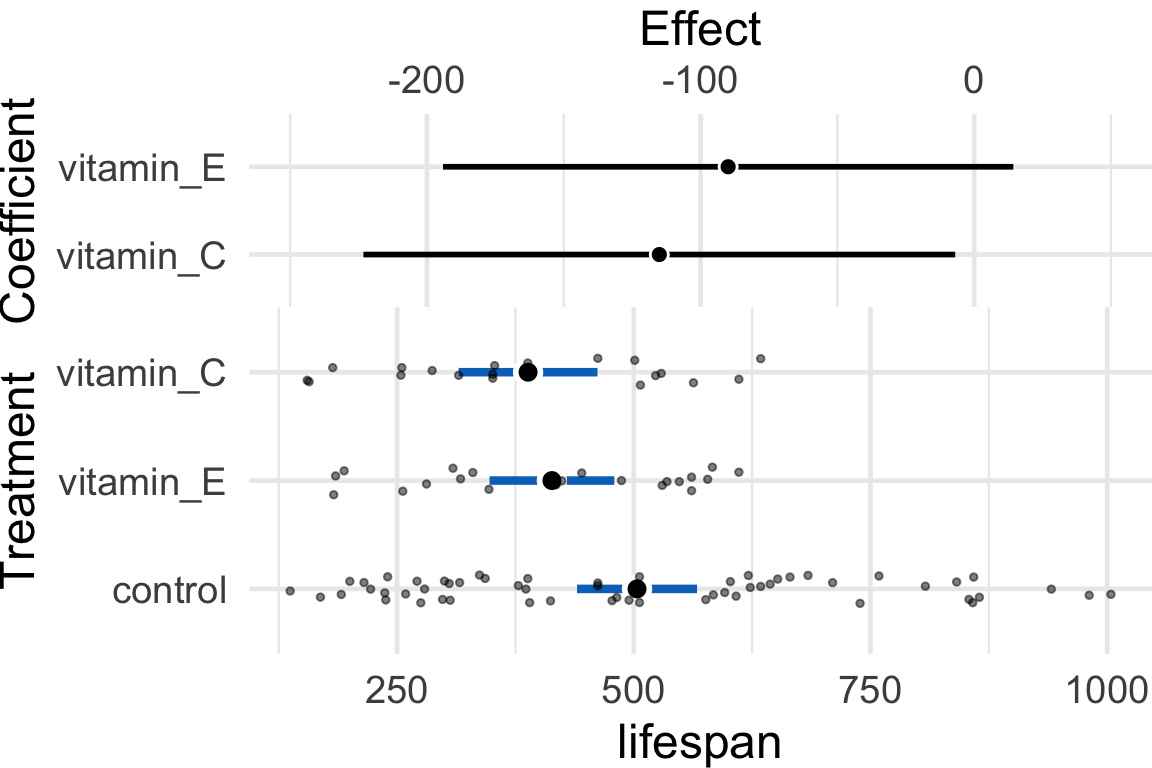
\includegraphics{Walker-elementary-statistical-modeling-draft_files/figure-latex/coldVoles-1.pdf}
\caption{\label{fig:coldVoles}HarrellPlot of vole data.}
\end{figure}

For the model fit to the data in Figure \ref{fig:line}B, the coefficient
of \(X\) is the slope of the line. Perhaps surprisingly, we can fit a
model like equation \eqref{eq:lm} to data in which the \(X\) variable is
categorical. A simple example is the experiment of antioxidants
(vitamins C and E) on lifespan in Voles (Fig. \ref{fig:coldVoles}). In
this experiment, the \(X\) variable is categorical, with three
\textbf{levels}: ``Control'', ``Vitamin\_E'' and ``Vitamin\_C''.
Categorical \(X\) variables are often called \textbf{factors}. The trick
to using a linear model with categorical \(X\) is to recode the factor
levels into numbers -- how this is done is explained in Chapter xxx.
When the \(X\) variable is categorical, the coefficients of the \(X\)
are \emph{differences in group means}. The linear model fit to the vole
data has two coefficients, one for Vitamin E and one for vitamin C. The
estimate and uncertainty of the these two coefficients are shown in the
top part of Figure \ref{fig:coldVoles}. The bottom part shows the raw
data, as well as the group (factor level) means and the uncertainty in
the estimate of these means.

The simplest possible model that can be fit to the data is

\begin{equation}
\mathrm{E}[Y] = b_0
\label{eq:unconditional}
\end{equation}

which is simply the mean of \(Y\), or, more specifically, the
\textbf{unconditional mean} of \(Y\), since its value is not conditional
on any value of \(X\).

\subsection{\texorpdfstring{``Statistical model'' not ``regression
model''}{Statistical model not regression model}}\label{statistical-model-not-regression-model}

Statistical modeling terminology can be confusing. The \(X\) variables
in a statistical model may be quantitative (continuous or integers) or
categorical (names or qualitative amounts) or some mix of the two.
Linear models with all quantitative independent variables are often
called ``regression models.'' Linear models with all categorical
independent variables are often called ``ANOVA models.'' Linear models
with a mix of quantitative and categorical variables are often called
``ANCOVA models'' if the focus is on one of the categorical \(X\) or
``regression models'' if there tend to be many independent variables.
Other patterns occur. For example ``ANCOVA models'' often include
interaction effects but ``regression models'' rarely do. To avoid
thinking of statistical analysis as ``regression vs.~ANOVA'', I will
most often use the term ``statistical model'' for general usage, and use
a more specific term only to emphasize something about the model in that
particluar context.

\section{Multilevel models}\label{multilevel-models}

\section{Linear models versus non-linear
models}\label{linear-models-versus-non-linear-models}

In this text, I use ``linear model'' for any model that is linear in the
parameters, which means that the different components of the model are
added together. Or, using the language of matrix algebra, the predictor
is a simple dot product of the model matrix and the coefficients. For
example, a cubic polynomial model

\begin{equation}
Y = \beta_0 + \beta_1 X + \beta_2 X^2 + \beta_3 X^3 + \varepsilon
\end{equation}

is a linear model, even though the function is non-linear, because the
different components are added (or, using matrix algebra, the predictor
is \(\mathbf{X}\boldsymbol{\beta}\)).

A generalized linear model (GLM) has the form \(g(\mu_i) = \eta_i\)
where \(\eta\) (the greek letter eta) is the linear predictor, which is
linear in the parameters.

\begin{equation}
\eta = \mathbf{X}\boldsymbol{\beta} 
\end{equation}

Many sources do not consider a GLM to be a ``linear model'' but an
``extension'' of a linear model. Regardless, a GLM is linear in the
parameters and here, I include GLMs under the ``linear model'' umbrella.

Non-linear models, in conrast to a GLM or classical linear model, are
not linear in the parameters (the predictor is not a simple dot product
of the model matrix and a vector of parameters). For example, the
Michaelis-Menten model is a nonlinear model

\begin{equation}
Y = \frac{\beta_1 X}{\beta_2 + X} + \varepsilon
\end{equation}

\chapter{Organization -- R Projects and R
Notebooks}\label{organization-r-projects-and-r-notebooks}

\section{Importing Packages}\label{importing-packages}

The R scripts you write will include functions in packages that are not
included in Base R. These packages need to be downloaded from an
internet server to your computer. You only need to do this once. But,
each time you start a new R session, you will need to load a package
using the \texttt{library()} function. Now is a good time to import
packages that we will use

\begin{enumerate}
\def\labelenumi{\arabic{enumi}.}
\tightlist
\item
  Open R Studio and choose the menu item ``Tools'' \textgreater{}
  ``Install Packages''
\item
  In the ``packages'' input box, insert ``ggplot2, data.table, emmeans,
  lme4, reshape2''. Make sure that ``install dependencies'' is clicked
  before you click ``Install''
\end{enumerate}

Again, once these are installed, you don't need to do this again. You
simply need to use the \texttt{library()} function at the start of a
script.

\section{Create an R Studio Project for this
Class}\label{create-an-r-studio-project-for-this-class}

\begin{enumerate}
\def\labelenumi{\arabic{enumi}.}
\tightlist
\item
  Create a folder named ``BIO\_413''
\item
  Within this folder, create new folders named

  \begin{enumerate}
  \def\labelenumii{\arabic{enumii}.}
  \tightlist
  \item
    ``notebooks'' -- this is where your R notebooks are stored
  \item
    ``R'' -- this is where R scripts are stored
  \item
    ``data'' -- this is where data that we download from public archives
    are stored
  \item
    ``output'' -- this is where you will store fake data generated in
    this class
  \item
    ``images'' -- this is where image files are stored
  \end{enumerate}
\item
  Open R Studio and click the menu item File \textgreater{} New
  Project\ldots{}
\item
  Choose ``Existing Directory'' and navigate to your BIO\_413 folder
\item
  Choose ``Create Project''
\item
  Check that a file named ``BIO\_413.Rproj'' is in your BIO\_413 folder
\end{enumerate}

\section{R Notebooks}\label{r-notebooks}

A typical statistical modeling project will consist of:

\begin{enumerate}
\def\labelenumi{\arabic{enumi}.}
\tightlist
\item
  reading data from Excel or text (.csv or .txt) files
\item
  cleaning data
\item
  analysis
\item
  generating plots
\item
  generating tables
\item
  writing text to describe the project, the methods, the analysis, and
  the interpretation of the results (plots and tables)
\end{enumerate}

The best practice for reproducible research is to have all six of these
steps in your R Notebook. Too many research projects are not
reproducible because the data were cleaned in Excel, and then different
parts of the data were separately imported into a GUI statistics
software for analysis, and then output from the statistics software was
transcribed to Excel to make a table. And other parts of the analysis
are used to create a plot in some plotting software. And then the tables
and plots are pasted into Microsoft Word to create a report. Any change
at any step in this process will require the researcher to remember all
the downstream parts that are dependent on the change and to re-do an
analysis, or a table, or a plot, etc. etc.

The goal with an R Studio Notebook is to explicitly link all this so
that changes in earlier steps automatically flow into the later steps.
So, at the end of a project, a researcher can choose ``run all'' from
the menu and the data are read, cleaned, analyzed, ploted, tabled, and
put into a report with the text.

This means that you have to think of the organization of the R code that
your write in a Notebook. Your cannot simply append new code to the end
of a script if something earlier (or above) is dependent on it. You need
to go back up and insert the new code at some earlier (and meaningful)
point.

For example, an R chunk generates 100 random normal values and then
plots these with a histogram. This was the chunk that I wrote

\begin{Shaded}
\begin{Highlighting}[]
\NormalTok{x <-}\StringTok{ }\KeywordTok{rnorm}\NormalTok{(n)}
\KeywordTok{qplot}\NormalTok{(x)}
\end{Highlighting}
\end{Shaded}

When I ran the chunk, I got the error ``Error in rnorm(n) : object n not
found''. I was using the function \texttt{rnorm()} to generate values
but I hadn't assigned any value to \texttt{n} yet, so I got the error.
To get this to work properly, I could have just typed
\texttt{n\ \textless{}-\ 100} in the console and then re-run the script
but I want it to work properly on a fresh run of the chunk (after
quitting and re-opening R Studio) so I instead inserted
\texttt{n\ \textless{}-\ 100} at the start of the chunk, like this:

\begin{Shaded}
\begin{Highlighting}[]
\NormalTok{n <-}\StringTok{ }\DecValTok{100}
\NormalTok{x <-}\StringTok{ }\KeywordTok{rnorm}\NormalTok{(n)}
\KeywordTok{qplot}\NormalTok{(x)}
\end{Highlighting}
\end{Shaded}

\subsection{Create an R Notebook for this
Chapter}\label{create-an-r-notebook-for-this-chapter}

\begin{enumerate}
\def\labelenumi{\arabic{enumi}.}
\tightlist
\item
  The top-left icon in R Studio is a little plus sign within a green
  circle. Click this and choose ``R Notebook'' from the pull-down menu.
\item
  Change the title of the notebook to ``Notebook\_01-organization''
\item
  Delete the default R Markdown text starting with ``This is an {[}R
  Markdown{]}\ldots{}''
\end{enumerate}

Now write some text documenting which packages you installed.

\subsection{\texorpdfstring{Create a ``setup''
chunk}{Create a setup chunk}}\label{create-a-setup-chunk}

\begin{enumerate}
\def\labelenumi{\arabic{enumi}.}
\tightlist
\item
  Click on the ``Insert'' menu on the right hand side of the script (R
  Markdown) pane and choose ``R''. This will insert an R code chunk into
  your R markdown document.
\item
  The first R chunk of a notebook should be a setup chunk. Name the
  chunk ``setup''
\item
  load the libraries ggplot2 and data.table and click the chunk's run
  button (the green triangle to the right of the chunk)
\end{enumerate}

\begin{Shaded}
\begin{Highlighting}[]
\KeywordTok{library}\NormalTok{(ggplot2)}
\KeywordTok{library}\NormalTok{(data.table)}
\end{Highlighting}
\end{Shaded}

I added the chunk option ``message=FALSE''. Run your chunk with and
without this as an option.

\subsection{\texorpdfstring{Create a ``simple plot''
chunk}{Create a simple plot chunk}}\label{create-a-simple-plot-chunk}

\begin{enumerate}
\def\labelenumi{\arabic{enumi}.}
\setcounter{enumi}{3}
\tightlist
\item
  Create a new chunk and label it ``simple plot''
\item
  insert the following R script and then click the chunk's run button.
  Do you get a plot?
\end{enumerate}

\begin{Shaded}
\begin{Highlighting}[]
\NormalTok{n <-}\StringTok{ }\DecValTok{100}
\NormalTok{x <-}\StringTok{ }\KeywordTok{rnorm}\NormalTok{(n)}
\KeywordTok{qplot}\NormalTok{(x)}
\end{Highlighting}
\end{Shaded}

\begin{verbatim}
## `stat_bin()` using `bins = 30`. Pick better value with `binwidth`.
\end{verbatim}

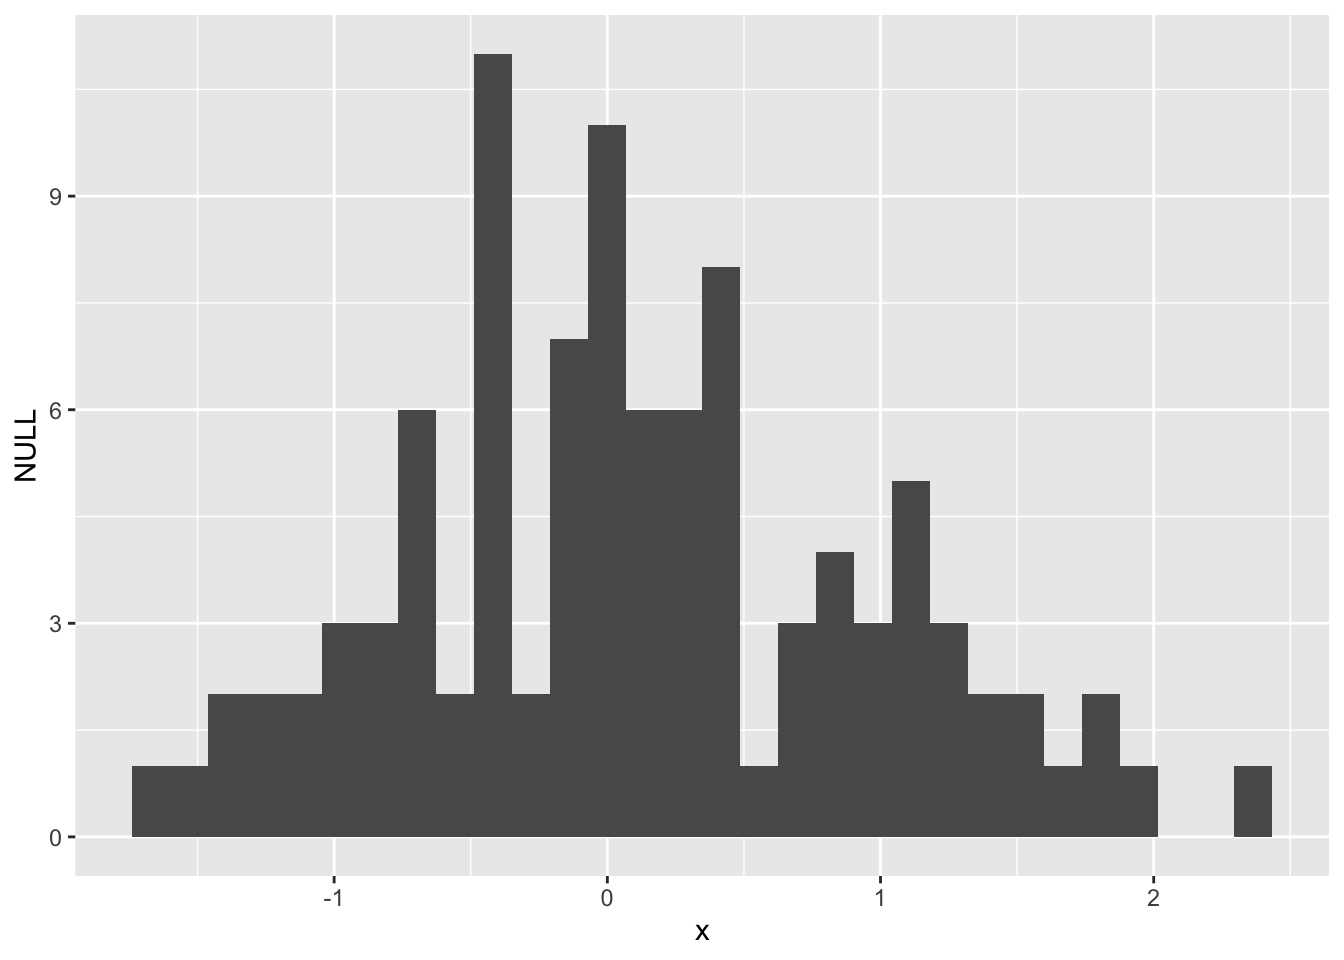
\includegraphics{Walker-elementary-statistical-modeling-draft_files/figure-latex/simple-plot-1.pdf}

\subsection{Create more R chunks and explore options and play with R
code}\label{create-more-r-chunks-and-explore-options-and-play-with-r-code}

\chapter{Data -- Reading, Writing, and
Fake}\label{data-reading-writing-and-fake}

\section{Create new notebook for this
chapter}\label{create-new-notebook-for-this-chapter}

Be sure to save the notebook in the ``notebooks'' folder of your
BIO\_413 project. Annotate your notebook with notes! Update it as you
learn more! We will use data.table for importing text files in
tab-delimited or comma-separated formats and the readxl package for
importing excel files.

\begin{Shaded}
\begin{Highlighting}[]
\KeywordTok{library}\NormalTok{(ggplot2)}
\KeywordTok{library}\NormalTok{(ggpubr)}
\KeywordTok{library}\NormalTok{(data.table)}
\KeywordTok{library}\NormalTok{(readxl)}
\KeywordTok{library}\NormalTok{(emmeans)}
\KeywordTok{library}\NormalTok{(mvtnorm)}

\NormalTok{knitr}\OperatorTok{::}\NormalTok{opts_chunk}\OperatorTok{$}\KeywordTok{set}\NormalTok{(}\DataTypeTok{fig.width=}\DecValTok{6}\NormalTok{, }\DataTypeTok{fig.height=}\DecValTok{4}\NormalTok{) }
\end{Highlighting}
\end{Shaded}

\section{Importing Data}\label{importing-data}

Throughout this book, we will download data from the
\href{https://datadryad.org}{Dryad Digital Repository}, which is a major
resource for increasing reproducibility in science. My own view is that
\emph{all data} should be archived on some public server (exceptions
include data that are proprietary or contain sensitive information --
such as human health measures).

The downloaded data will be inserted into the ``data'' folder. To access
these data in an R script, the script needs to know ``where to look'' or
the ``address.'' This address is the \textbf{directory path}. The
default path for an R notebook is the directory containing the notebook
.Rmd file. This file should be in the ``notebooks'' folder within
``BIO\_413''. The ``BIO\_413'' Folder is the parent of the ``notebooks''
folder. It is also the parent of the ``data'' folder. To see any content
within the ``data'' folder, the R script needs to tell R to move back
(or up) the directory structure out of the ``notebooks'' folder into the
parent ``BIO\_413'' folder and then forward (or down) into the ``data''
folder. This is done with

\begin{Shaded}
\begin{Highlighting}[]
\NormalTok{data_path <-}\StringTok{ "../data"}
\end{Highlighting}
\end{Shaded}

The \texttt{..} moves the address (of where to read input or write
output) back one step and \texttt{/data} moves the address forward into
the ``data'' folder. This folder will eventually contains lots of data
from Dryad Digital Repository.

\subsection{Excel File}\label{excel-file}

The Excel dataset is from an experiment on the growth response of zebra
finch chicks to an incubation call that presumably signals ``hot
environment'' to the embryos
(\href{http://science.sciencemag.org/content/353/6301/812}{Mariette,
M.M. and Buchanan, K.L., 2016. Prenatal acoustic communication programs
offspring for high posthatching temperatures in a songbird. Science,
353(6301), pp.812-814}). The source file is from the Dryad Repository
here:

\textbf{file name}: ``allDatasetsMarietteBuchanan2016.xls''

\textbf{source}: \url{https://datadryad.org//handle/10255/dryad.122315}

Steps

\begin{enumerate}
\def\labelenumi{\arabic{enumi}.}
\tightlist
\item
  Copy the title of the Dryad page, which is ``Data from: Prenatal
  acoustic communication programs offspring for high post-hatching
  temperatures in a songbird''
\item
  Create a new folder within ``data'' and paste in the copied title as
  the folder name
\item
  Remove the colon from the name, so the folder name is ``Data from
  Prenatal acoustic communication programs offspring for high
  post-hatching temperatures in a songbird''
\item
  Download the .xls file into this folder
\end{enumerate}

A .xls file is an old (pre 2007) Microsoft Excel file type. It is a
binary file and can only be opened into a readable format with
specialized software. The more modern Excel file type is .xlsx, which
contains within it multiple xml components. An xml file is a text file,
and so contains readable content, but the content is xml code to display
something. In general, I am a big advocate of archiving stuff as text
files (manuscripts, data, scripts, blog posts) because these will
\emph{always} be readable by future software. Microsoft Excel is not
likely to die anytime soon and software that can read .xls and
especially .xlsx files (again, .xlsx files are text files) is even less
likely to disappear but we can feel even more confident if data are
archived as text files. That said, a single microsoft excel file with
multiple sheets is an efficient method for distributing data and the
readxl package provides excellent tools for reading different sheets of
a single .xls or .xlsx file.

The code below uses the function \texttt{read\_excel()} from the package
readxl. More about the amazing power of this package is the
\href{https://readxl.tidyverse.org}{tidyverse page} and
\href{http://r4ds.had.co.nz/data-import.html}{chapter 11} in the \emph{R
for Data Science} book.

\begin{Shaded}
\begin{Highlighting}[]
\NormalTok{data_folder <-}\StringTok{ "Data from Prenatal acoustic communication programs offspring for high post-hatching temperatures in a songbird"}
\NormalTok{filename <-}\StringTok{ "allDatasetsMarietteBuchanan2016.xls"}
\NormalTok{file_path <-}\StringTok{ }\KeywordTok{paste}\NormalTok{(data_path, data_folder, filename, }\DataTypeTok{sep=}\StringTok{"/"}\NormalTok{)}
\NormalTok{chick <-}\StringTok{ }\KeywordTok{data.table}\NormalTok{(}\KeywordTok{read_excel}\NormalTok{(file_path, }\DataTypeTok{sheet=}\StringTok{"nestlingMass"}\NormalTok{))}
\KeywordTok{head}\NormalTok{(chick) }\CommentTok{# check -- are there headers? are there the correct number of columns?}
\end{Highlighting}
\end{Shaded}

\begin{verbatim}
##       chick ID brood ID brood composition sex rank in nest
## 1:    N1.10LF3  N1.10m3             mixed   F            2
## 2: N1.10noCut3  N1.10m3             mixed   M            4
## 3:    N1.10RB3  N1.10m3             mixed   F            2
## 4:    N1.10RF3  N1.10m3             mixed   F            5
## 5:    N1.12LB3  N1.12m3             mixed   F            3
## 6:    N1.12LF3  N1.12m3             mixed   F            1
##    playback treatment nest temperature above ambient
## 1:              treat                       4.289583
## 2:               cont                       4.289583
## 3:               cont                       4.289583
## 4:               cont                       4.289583
## 5:               cont                       3.972917
## 6:              treat                       3.972917
##    max daily temp hatch day mean max temp hatch to day2
## 1:                     17.4                    18.83333
## 2:                     19.0                    20.53333
## 3:                     17.4                    18.83333
## 4:                     19.0                    20.53333
## 5:                     29.0                    24.63333
## 6:                     25.1                    24.80000
##    mean max temp hatch to day10 mean max temp hatch to day13 hatching mass
## 1:                        22.70                     23.05714           0.7
## 2:                        24.53                     23.41429           0.6
## 3:                        22.70                     23.05714           0.7
## 4:                        24.53                     23.41429           0.6
## 5:                        22.85                     22.91429           0.7
## 6:                        23.35                     23.24286           0.6
##              day1 mass           day2 mass         day10 mass day13 mass
## 1:  1.1000000000000001                 1.2                 NA        9.8
## 2: 0.80000000000000004  1.1000000000000001                 NA        9.1
## 3: 0.90000000000000002  1.3999999999999999                 NA        9.3
## 4:                 0.5 0.90000000000000002                 NA        7.7
## 5:                   1  1.3999999999999999 9.4000000000000004       10.1
## 6: 0.90000000000000002  1.3999999999999999 8.0999999999999996        9.6
##    day13 tarsus
## 1:        14.11
## 2:        12.90
## 3:        13.60
## 4:        13.06
## 5:        14.08
## 6:        13.46
\end{verbatim}

\begin{center}\rule{0.5\linewidth}{\linethickness}\end{center}

\textbf{NOTE}

If you are getting errors when trying to read a file, it is probably a
bug in the construction of the variable \texttt{file\_path}, which is a
string variable and the value has to be exactly match the directly path
to the file you are trying to read. \texttt{file\_path} is constructed
by pasting together the variables \texttt{data\_path},
\texttt{data\_folder}, and \texttt{filename}. Type \texttt{file\_path}
into the console and look at the value. Then check

\begin{enumerate}
\def\labelenumi{\arabic{enumi}.}
\tightlist
\item
  Spelling. Humans are very good at understanding misspelled words but
  the R language (or any computer language) is very literal. ``../data''
  does not equal ``./data'' or ``../ data'' or ``../data''
\item
  Capitalization. R is \textbf{case sensitive} (some programming
  languages are not). ``../data'' does not equal ``../Data'' or
  ``../DATA''.
\item
  is the file you are trying to read actually in the folder you are
  trying to read from?
\item
  is the notebook that you are writing in the folder ``notebooks''? (the
  construction of \texttt{file\_path} assumes that notebook is one
  folder deep within the project folder.
\end{enumerate}

If the spelling or capitalization of any of these components is wrong,
then \texttt{file\_path} will be wrong. If there is any difference in
any character in the string, then R will return an error. So spelling
AND capitalization have to be perfect, not simply close. Humans are very
good at understanding misspelled and OdDLy capitalized words but the R
language (or any computer language) is very literal.

\begin{center}\rule{0.5\linewidth}{\linethickness}\end{center}

In this book, we will consistently uses the protocol for storing and
retrieving downloaded files. The first three lines in the script above
creates the directory path to the file. This path includes

\begin{enumerate}
\def\labelenumi{\arabic{enumi}.}
\tightlist
\item
  data\_path -- the relative path into the folder ``data'' (relative to
  the location of the notebook file)
\item
  data\_folder -- the name of the folder within ``data'' containing the
  file
\item
  filename -- the name of the file to read
\end{enumerate}

These are all put together into a single path using the function
\texttt{paste()}. Read about paste. It will be used repeatedly. The
\texttt{read\_excel(file\_path,\ sheet="nestlingMass")} reads the
nestlingMass sheet only. This function is embedded within the
\texttt{data.table()} function and so is converted into a data.table.
The data.table is assigned to the object ``chick''

The \texttt{head(chick)} script simply displays the first few lines of
the data.table. This is one way to check that the data were imported
correctly. In this case, it is easy to see that the column names have
spaces in them. It can sometimes be hard to work with column names with
spaces and so this next line of code changes all spaces to an underscore

\begin{Shaded}
\begin{Highlighting}[]
\KeywordTok{setnames}\NormalTok{(chick, }\DataTypeTok{old=}\KeywordTok{colnames}\NormalTok{(chick), }\DataTypeTok{new=}\KeywordTok{gsub}\NormalTok{(}\StringTok{" "}\NormalTok{, }\StringTok{"_"}\NormalTok{, }\KeywordTok{colnames}\NormalTok{(chick)))}
\end{Highlighting}
\end{Shaded}

Resist the temptation to change the column names in the data file, which
reduces reproducibility. Always increase reproducibility!

Just for fun, let's plot the data and reproduce Fig. 2A and B. We are
using the \texttt{qplot} function, which is from the ggplot2 package.
Two plots are made and only a subset of the rows are plotted in each (in
A, the subset in which playback\_treatment==``treat'' and, in B, the
subset in which playback\_treatment==``cont''). This book uses the
ggplot2 package extensively.

\begin{Shaded}
\begin{Highlighting}[]
\KeywordTok{qplot}\NormalTok{(}\DataTypeTok{x=}\NormalTok{nest_temperature_above_ambient, }\DataTypeTok{y=}\NormalTok{day13_mass, }\DataTypeTok{data=}\NormalTok{chick[playback_treatment}\OperatorTok{==}\StringTok{"treat"}\NormalTok{]) }\OperatorTok{+}
\StringTok{  }\KeywordTok{geom_smooth}\NormalTok{(}\DataTypeTok{method=}\StringTok{"lm"}\NormalTok{)}
\end{Highlighting}
\end{Shaded}

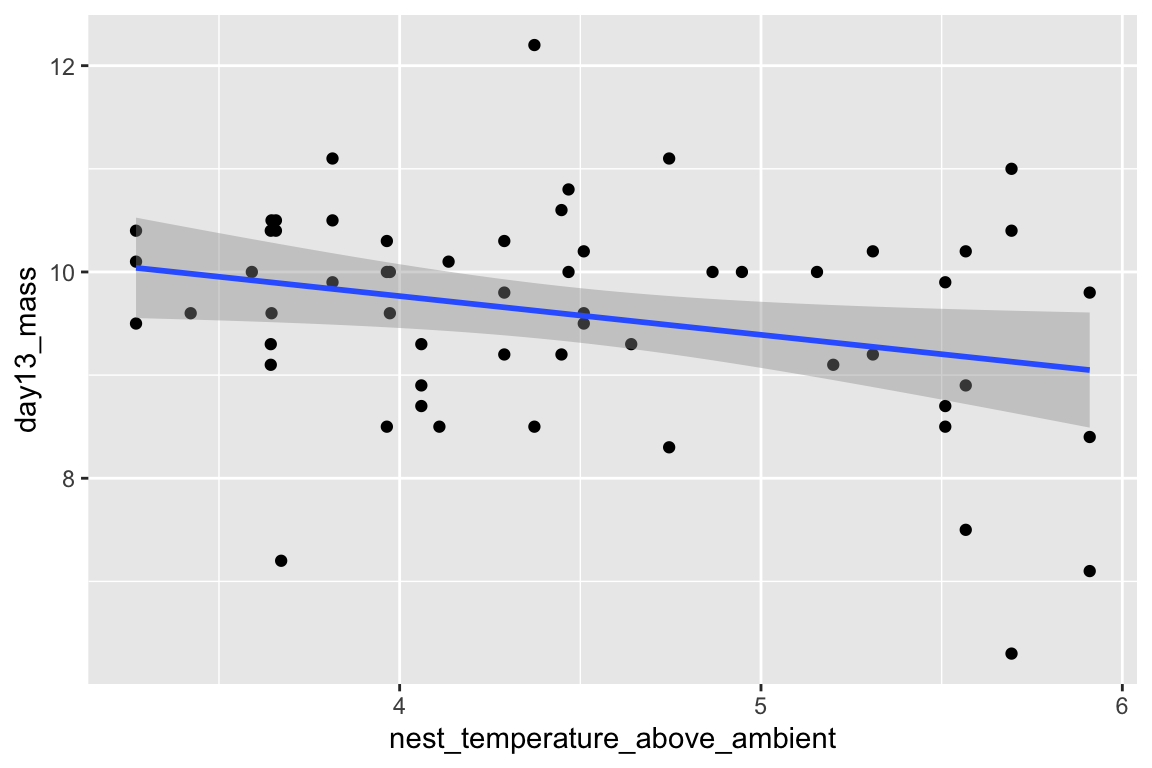
\includegraphics{Walker-elementary-statistical-modeling-draft_files/figure-latex/plotchickdata-1.pdf}

\begin{Shaded}
\begin{Highlighting}[]
\KeywordTok{qplot}\NormalTok{(}\DataTypeTok{x=}\NormalTok{nest_temperature_above_ambient, }\DataTypeTok{y=}\NormalTok{day13_mass, }\DataTypeTok{data=}\NormalTok{chick[playback_treatment}\OperatorTok{==}\StringTok{"cont"}\NormalTok{]) }\OperatorTok{+}
\StringTok{  }\KeywordTok{geom_smooth}\NormalTok{(}\DataTypeTok{method=}\StringTok{"lm"}\NormalTok{)}
\end{Highlighting}
\end{Shaded}

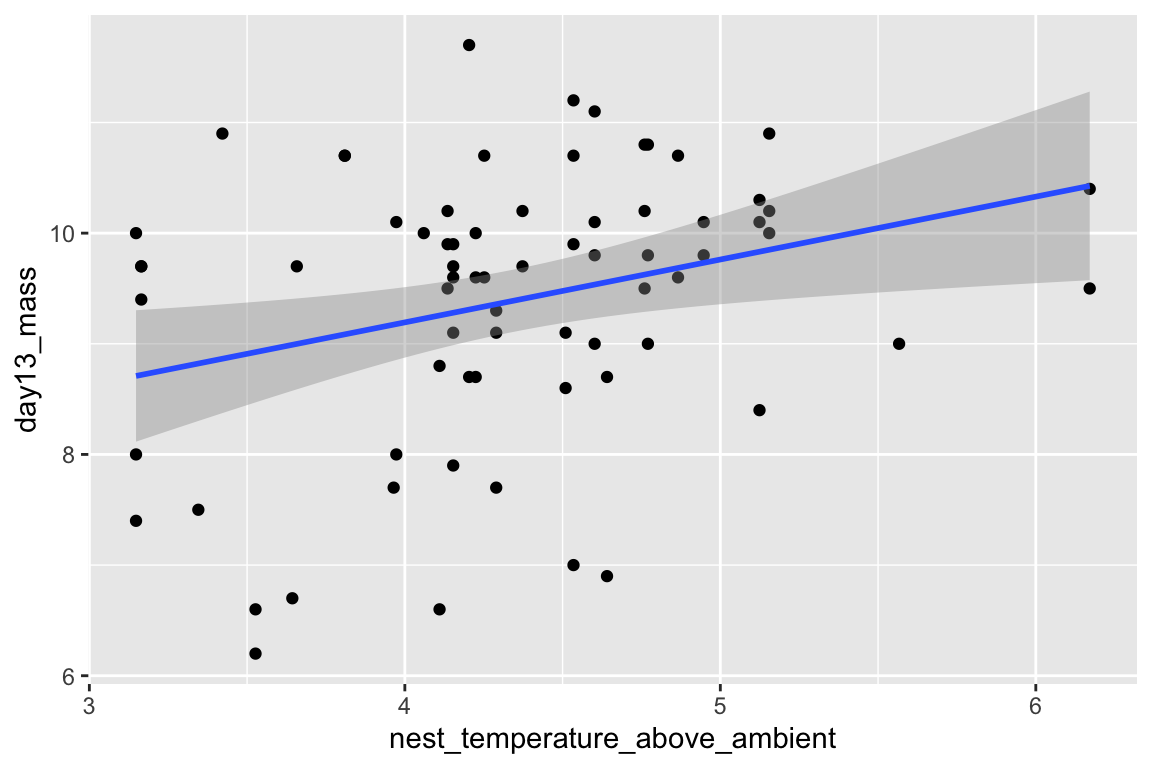
\includegraphics{Walker-elementary-statistical-modeling-draft_files/figure-latex/plotchickdata-2.pdf}

\subsection{Text File}\label{text-file}

The example dataset comes from an experiment on the effect of
\href{http://science.sciencemag.org/content/early/2012/03/28/science.1215025}{neonicotinoid
pesticides on bumble bee colony growth}.

\textbf{file name}: ``Whitehorn, O'Connor, Wackers, Goulson (2012) Data
from `Neonicotinoid pesticide reduces bumblebee colony growth and queen
production'.csv.csv''

\textbf{source}:
\url{https://datadryad.org//resource/doi:10.5061/dryad.1805c973}

Steps

\begin{enumerate}
\def\labelenumi{\arabic{enumi}.}
\tightlist
\item
  Copy the title of the Dryad page, which is ``Data from: Neonicotinoid
  pesticide reduces bumblebee colony growth and queen production''
\item
  Create a new folder within ``data'' and paste in the copied title as
  the folder name
\item
  Remove the colon from the name, so the folder name is ``Data from
  Neonicotinoid pesticide reduces bumblebee colony growth and queen
  production''
\item
  Download the .csv file into this folder
\end{enumerate}

A .csv file is a text file that is comma-delimted, which means that the
entries of a row are separated by commas. A text file is readable by any
text editor software and most other kinds of software. Datasets that are
stored as text files are typically saved as either .csv (where the
entries of a row are separated by commas) or .txt (where the entries are
separated by tabs). The base R way to read a .csv file is using
\texttt{read.csv}. The \texttt{read.table} function is more versatile,
as the delimiter can be specified. The function \texttt{fread()} from
the data.table package is fast, smart, and flexible. It is smart in the
sense that it guesses what the delimter is. Unfortunately, because of
spaces in the column labels for this file, fread guesses incorrectly
(another reason why spaces in column labels should be avoided). To
overcome this, the statement below specifies that the file contains a
``header'' (a line containing column labels)

\begin{Shaded}
\begin{Highlighting}[]
\NormalTok{data_folder <-}\StringTok{ "Data from Neonicotinoid pesticide reduces bumblebee colony growth and queen production"}
\NormalTok{filename <-}\StringTok{ "Whitehorn, O'Connor, Wackers, Goulson (2012) Data from 'Neonicotinoid pesticide reduces bumblebee colony growth and queen production'.csv.csv"}
\NormalTok{file_path <-}\StringTok{ }\KeywordTok{paste}\NormalTok{(data_path, data_folder, filename, }\DataTypeTok{sep=}\StringTok{"/"}\NormalTok{)}
\NormalTok{bee <-}\StringTok{ }\KeywordTok{fread}\NormalTok{(file_path, }\DataTypeTok{header=}\OtherTok{TRUE}\NormalTok{)}
\NormalTok{bee[, Treatment}\OperatorTok{:}\ErrorTok{=}\KeywordTok{factor}\NormalTok{(Treatment, }\KeywordTok{c}\NormalTok{(}\StringTok{"Control"}\NormalTok{, }\StringTok{"Low"}\NormalTok{, }\StringTok{"High"}\NormalTok{))]}
\KeywordTok{head}\NormalTok{(bee)}
\end{Highlighting}
\end{Shaded}

\begin{verbatim}
##    Treatment Nest ID No. workers      0      1      2   3   4    5    6
## 1:   Control      C1          13 712.95 748.30 800.57 865 966  997  850
## 2:   Control      C2          14 719.58 750.00 789.25 822 812  846  827
## 3:   Control      C3          17 704.92 736.31 767.99 837 976 1117 1050
## 4:   Control      C4          20 726.42 763.31 795.60 813 801  784   NA
## 5:   Control      C5          28 740.60 785.52 808.42 837 871  906  886
## 6:   Control      C6          15 727.10 751.90 774.80 807 847  859  827
##      7   8 V13 Workers left Males New queens Total unhatched pupae
## 1: 791 775  NA            2     0          1                    NA
## 2: 820 802  NA            6    15          0                    20
## 3: 866 808  NA            1     0          9                    NA
## 4:  NA  NA  NA            0     0          0                    12
## 5: 807 775  NA            3     0          0                    NA
## 6:  NA  NA  NA            0     0          0                   118
##    Queen pupae Empty cells
## 1:          NA          NA
## 2:           0         120
## 3:          NA          NA
## 4:           0          72
## 5:          NA          NA
## 6:          20         132
\end{verbatim}

Here, as with the import of the Excel file, the first three lines create
the directory path to the file. The treatment column is a factor
variable containing three levels (Control, Low, and High). R
automatically orders these alphabetically. For plotting and analysis, we
might want a different order. For example, we want Control to be first
in the order, since this is a natural ``reference'' level (what
everything is compared to). And if we think of ``Control'' as no
treatment, then it makes sense to have ``Low'' second in order and
``Hight'' last in order. The line
\texttt{bee{[},\ Treatment:=factor(Treatment,\ c("Control",\ "Low",\ "High")){]}}
re-orders these levels to this more meaningful order.

Again, there are spaces in the column names. \textbf{Here I'll leave it
to you to change this}

Here is a reproduction of Fig 2.

\begin{Shaded}
\begin{Highlighting}[]
\KeywordTok{ggbarplot}\NormalTok{(}\DataTypeTok{data=}\NormalTok{bee, }\DataTypeTok{x=}\StringTok{"Treatment"}\NormalTok{, }\DataTypeTok{y=}\StringTok{"New_queens"}\NormalTok{, }\DataTypeTok{add =} \KeywordTok{c}\NormalTok{(}\StringTok{"mean_se"}\NormalTok{))}
\end{Highlighting}
\end{Shaded}

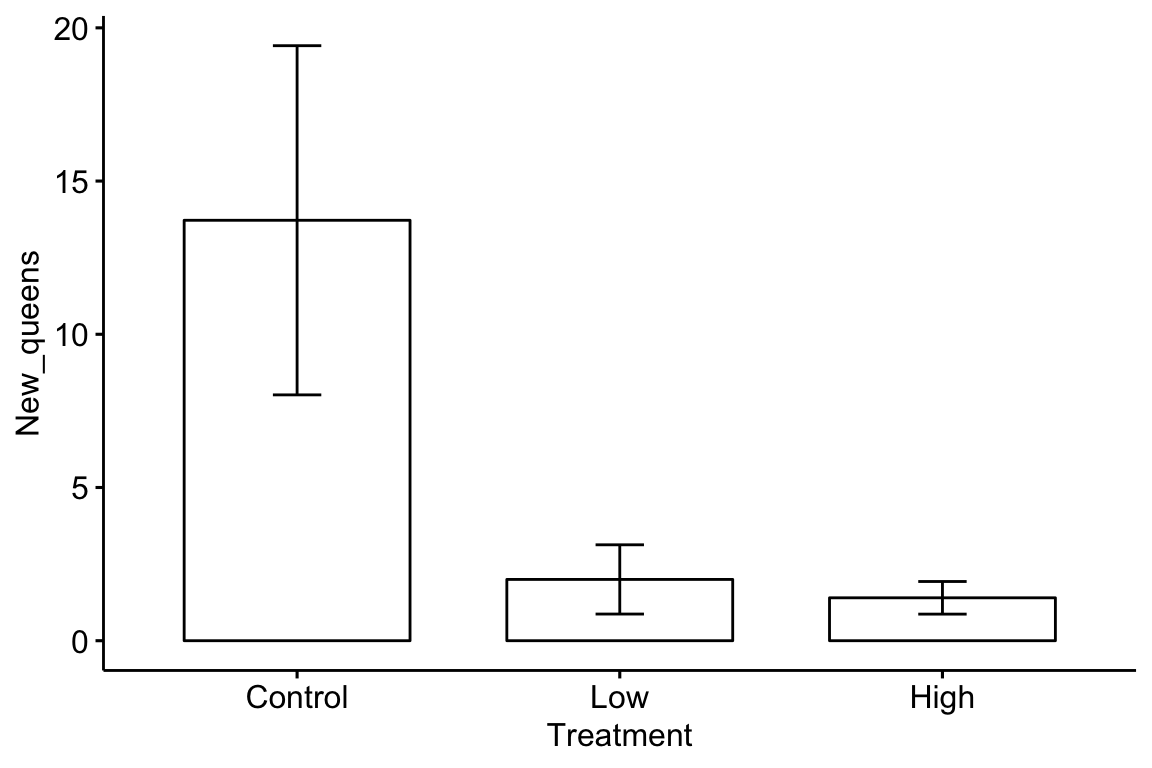
\includegraphics{Walker-elementary-statistical-modeling-draft_files/figure-latex/plot-bee-fig-2-1.pdf}

The plot suggests immediately some problems with the plot itself and the
associated analysis. First, the y-axis is counts, which means that
negative values are impossible. But the standard error bars look like
they use standard errors computed from a model that allows infinetly
large negative values, and the illustrated standard error bars imply
that negative values exist. So these error bars are misleading. Second,
it is good practice, especially if sample sizes are modest or small, to
``show the data'', which means, show the individual data points and not
just a summary of the distribution.

Here are three alternative plots for exploratory purposes. The first
simply ``shows the data'' but still uses the misleading standard error
bars. The second uses a box plot. The last plots the means and 95\%
confidence intervals modeled with a GLM (generalized linear model) to
account for the count data (the model used could be improved). Notice
that the bar length above the mean is longer than the bar length below
the mean (that is the interval is asymmetric about the mean). In order
to stay focussed on importing data, I leave explanation of these plots
and analysis to later chapters.

\begin{Shaded}
\begin{Highlighting}[]
\KeywordTok{ggbarplot}\NormalTok{(}\DataTypeTok{data=}\NormalTok{bee, }\DataTypeTok{x=}\StringTok{"Treatment"}\NormalTok{, }\DataTypeTok{y=}\StringTok{"New_queens"}\NormalTok{, }\DataTypeTok{add =} \KeywordTok{c}\NormalTok{(}\StringTok{"mean_se"}\NormalTok{, }\StringTok{"point"}\NormalTok{))}
\end{Highlighting}
\end{Shaded}

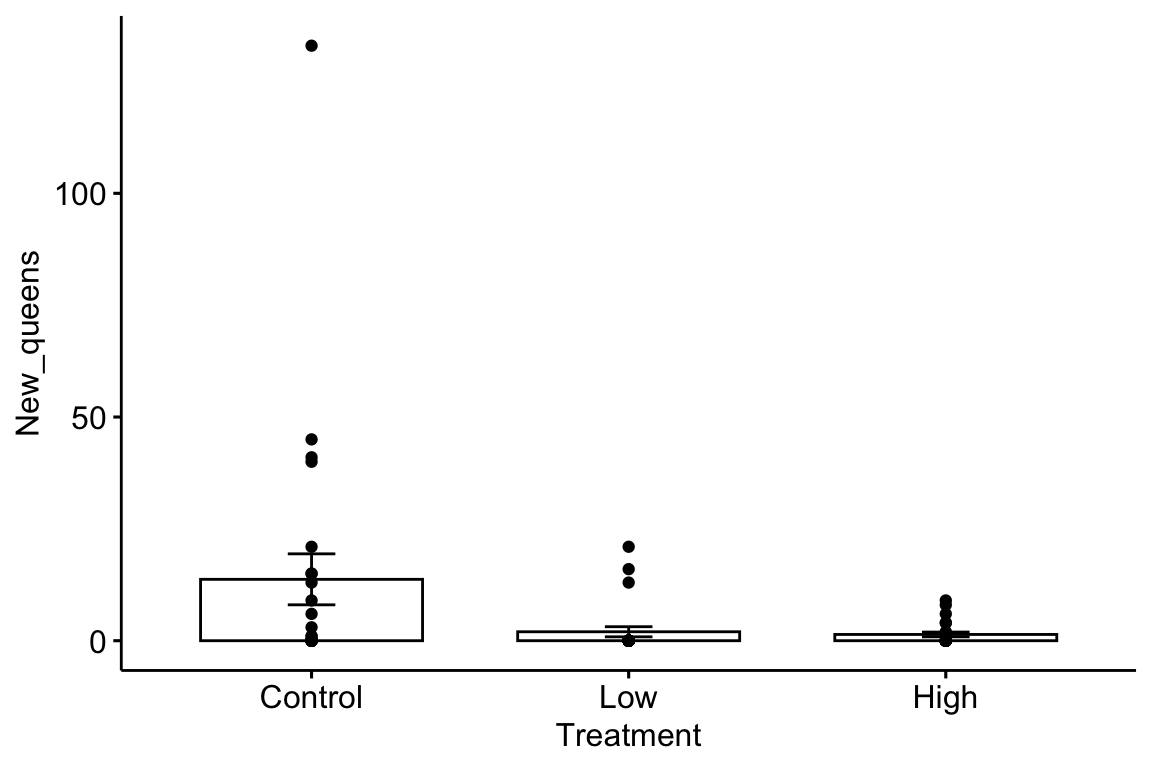
\includegraphics{Walker-elementary-statistical-modeling-draft_files/figure-latex/alternative-plots-1.pdf}

\begin{Shaded}
\begin{Highlighting}[]
\KeywordTok{ggboxplot}\NormalTok{(}\DataTypeTok{data=}\NormalTok{bee, }\DataTypeTok{x=}\StringTok{"Treatment"}\NormalTok{, }\DataTypeTok{y=}\StringTok{"New_queens"}\NormalTok{)}
\end{Highlighting}
\end{Shaded}

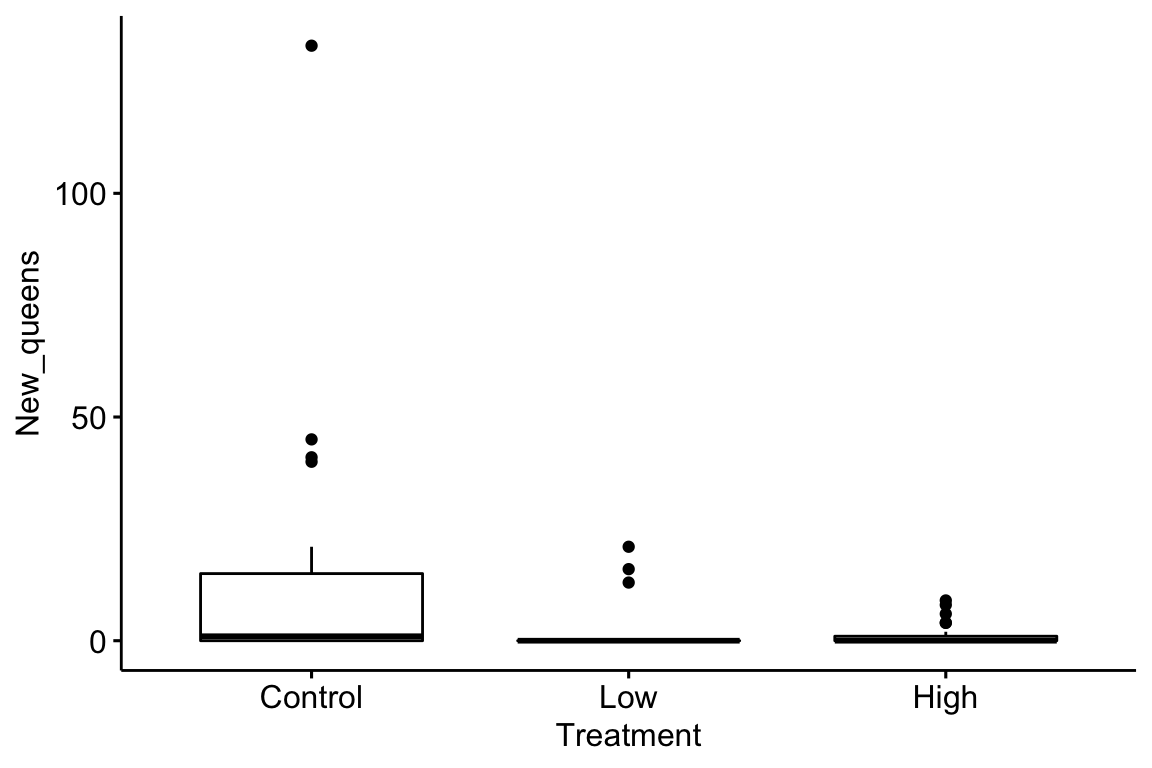
\includegraphics{Walker-elementary-statistical-modeling-draft_files/figure-latex/alternative-plots-2.pdf}

\begin{Shaded}
\begin{Highlighting}[]
\NormalTok{fit.glm <-}\StringTok{ }\KeywordTok{glm}\NormalTok{(New_queens }\OperatorTok{~}\StringTok{ }\NormalTok{Treatment, }\DataTypeTok{data=}\NormalTok{bee, }\DataTypeTok{family=}\KeywordTok{poisson}\NormalTok{())}
\NormalTok{means.glm <-}\StringTok{ }\KeywordTok{emmeans}\NormalTok{(fit.glm, }\DataTypeTok{specs=}\StringTok{"Treatment"}\NormalTok{, }\DataTypeTok{type =} \StringTok{"response"}\NormalTok{)}
\NormalTok{gg <-}\StringTok{ }\KeywordTok{ggplot}\NormalTok{(}\DataTypeTok{data=}\KeywordTok{data.frame}\NormalTok{(means.glm), }\KeywordTok{aes}\NormalTok{(}\DataTypeTok{x=}\NormalTok{Treatment, }\DataTypeTok{y=}\NormalTok{rate)) }\OperatorTok{+}
\StringTok{  }\KeywordTok{geom_col}\NormalTok{(}\DataTypeTok{fill=}\StringTok{"gray"}\NormalTok{) }\OperatorTok{+}\StringTok{ }
\StringTok{  }\KeywordTok{geom_errorbar}\NormalTok{(}\KeywordTok{aes}\NormalTok{(}\DataTypeTok{x=}\NormalTok{Treatment, }\DataTypeTok{ymin=}\NormalTok{asymp.LCL, }\DataTypeTok{ymax=}\NormalTok{asymp.UCL), }\DataTypeTok{width=}\FloatTok{0.3}\NormalTok{) }\OperatorTok{+}
\StringTok{  }\KeywordTok{ylab}\NormalTok{(}\StringTok{"New queens"}\NormalTok{) }\OperatorTok{+}
\StringTok{  }\OtherTok{NULL}
\NormalTok{gg}
\end{Highlighting}
\end{Shaded}

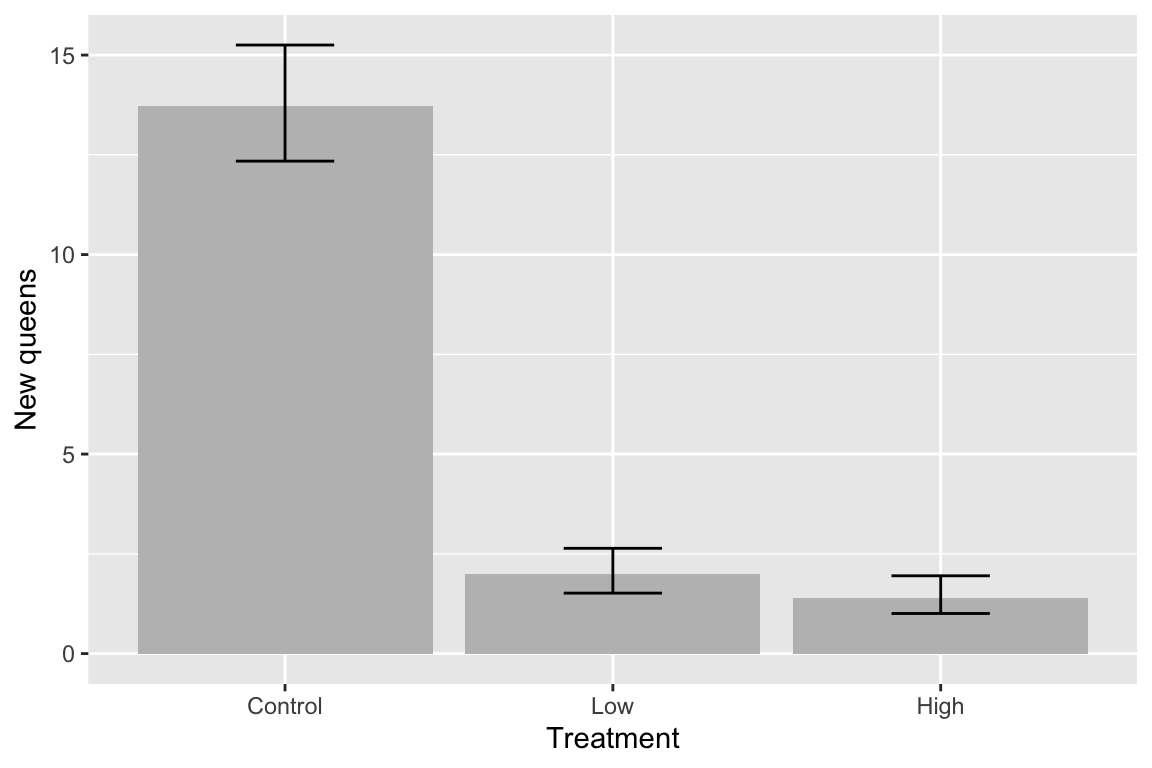
\includegraphics{Walker-elementary-statistical-modeling-draft_files/figure-latex/alternative-plots-3.pdf}

\section{Creating Fake Data}\label{creating-fake-data}

\subsection{Continuous X (fake observational
data)}\label{continuous-x-fake-observational-data}

A very simple simulation of a regression model

\begin{Shaded}
\begin{Highlighting}[]
\NormalTok{n <-}\StringTok{ }\DecValTok{25}
\NormalTok{beta_}\DecValTok{0}\NormalTok{ <-}\StringTok{ }\DecValTok{25}
\NormalTok{beta_}\DecValTok{1}\NormalTok{ <-}\StringTok{ }\FloatTok{3.4}
\NormalTok{sigma <-}\StringTok{ }\DecValTok{2}
\NormalTok{x <-}\StringTok{ }\KeywordTok{rnorm}\NormalTok{(n)}
\NormalTok{y <-}\StringTok{ }\NormalTok{beta_}\DecValTok{0} \OperatorTok{+}\StringTok{ }\NormalTok{beta_}\DecValTok{1}\OperatorTok{*}\NormalTok{x }\OperatorTok{+}\StringTok{ }\KeywordTok{rnorm}\NormalTok{(n, }\DataTypeTok{sd=}\NormalTok{sigma)}
\KeywordTok{qplot}\NormalTok{(x, y)}
\end{Highlighting}
\end{Shaded}

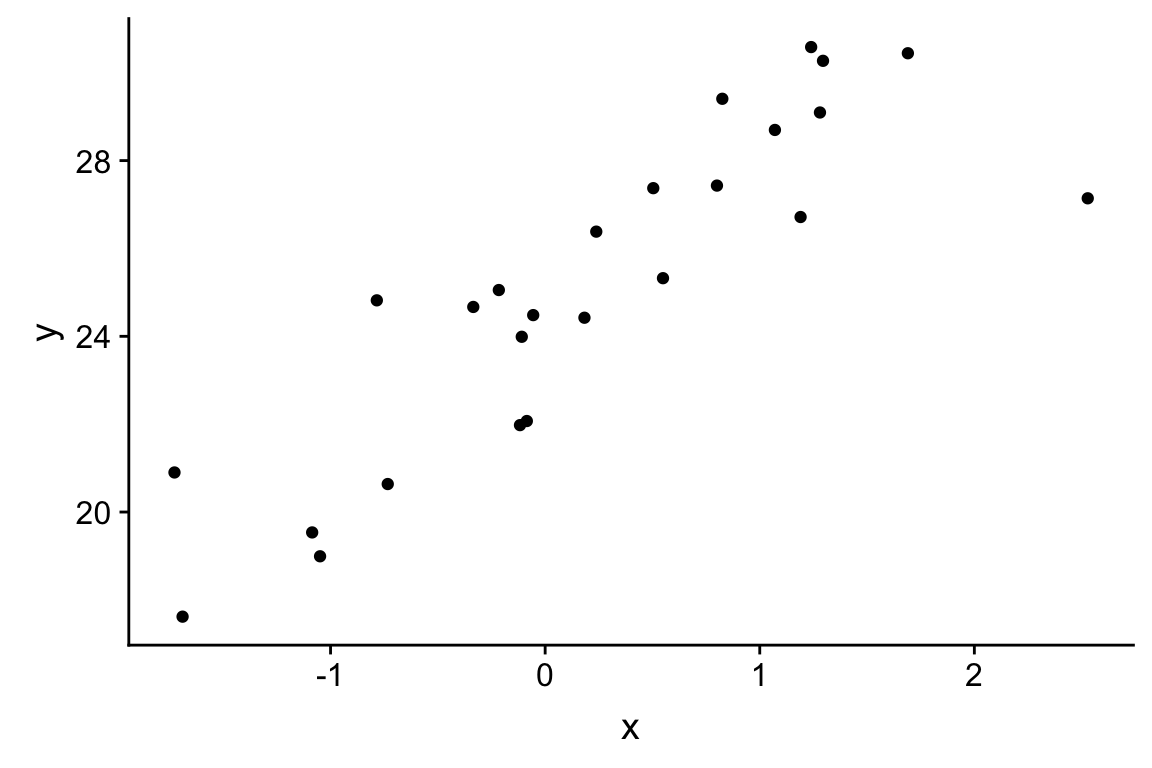
\includegraphics{Walker-elementary-statistical-modeling-draft_files/figure-latex/continuous-X-1.pdf}

\begin{Shaded}
\begin{Highlighting}[]
\NormalTok{knitr}\OperatorTok{::}\KeywordTok{kable}\NormalTok{(}\KeywordTok{coefficients}\NormalTok{(}\KeywordTok{summary}\NormalTok{(}\KeywordTok{lm}\NormalTok{(y }\OperatorTok{~}\StringTok{ }\NormalTok{x))), }\DataTypeTok{digits=}\DecValTok{2}\NormalTok{)}
\end{Highlighting}
\end{Shaded}

\begin{tabular}{l|r|r|r|r}
\hline
  & Estimate & Std. Error & t value & Pr(>|t|)\\
\hline
(Intercept) & 24.46 & 0.39 & 62.43 & 0\\
\hline
x & 3.05 & 0.37 & 8.25 & 0\\
\hline
\end{tabular}

The coefficient of \(x\) is the ``Estimate''. How close is the estimate?
Run the simulation several times to look at the variation in the
estimate -- this will give you a sense of the uncertainty. Increase
\(n\) and explore this uncertainty. Increase all the way up to
\(n=10^5\). Commenting out the qplot line will make this exploration
easier.

\subsection{Categorical X (fake experimental
data)}\label{categorical-x-fake-experimental-data}

\begin{Shaded}
\begin{Highlighting}[]
\NormalTok{n <-}\StringTok{ }\DecValTok{5}

\NormalTok{fake_data <-}\StringTok{ }\KeywordTok{data.table}\NormalTok{(}\DataTypeTok{Treatment=}\KeywordTok{rep}\NormalTok{(}\KeywordTok{c}\NormalTok{(}\StringTok{"control"}\NormalTok{, }\StringTok{"treated"}\NormalTok{), }\DataTypeTok{each=}\NormalTok{n))}
\NormalTok{beta_}\DecValTok{0}\NormalTok{ <-}\StringTok{ }\FloatTok{10.5} \CommentTok{# mean of untreated}
\NormalTok{beta_}\DecValTok{1}\NormalTok{ <-}\StringTok{ }\FloatTok{2.1} \CommentTok{# difference in means (treated - untreated)}
\NormalTok{sigma <-}\StringTok{ }\DecValTok{3} \CommentTok{# the error standard deviation}
\CommentTok{# the Y variable ("Response") is a function of treatment. We use some matrix}
\CommentTok{# algebra to get this done.}
\CommentTok{# Turn the Treatment assignment into a model matrix. Take a peak at X!}
\NormalTok{X <-}\StringTok{ }\KeywordTok{model.matrix}\NormalTok{(}\OperatorTok{~}\StringTok{ }\NormalTok{Treatment, fake_data)}
\CommentTok{# to make the math easier the coefficients are collected into a vector}
\NormalTok{beta <-}\StringTok{ }\KeywordTok{c}\NormalTok{(beta_}\DecValTok{0}\NormalTok{, beta_}\DecValTok{1}\NormalTok{)}
\CommentTok{# you will see the formula Y=Xb many times. Here it is coded in R}
\NormalTok{fake_data[, Response}\OperatorTok{:}\ErrorTok{=}\NormalTok{X}\OperatorTok\NormalTok{beta }\OperatorTok{+}\StringTok{ }\KeywordTok{rnorm}\NormalTok{(n, }\DataTypeTok{sd=}\NormalTok{sigma)]}
\CommentTok{# plot it with a strip chart (often called a "dot plot")}
\KeywordTok{ggstripchart}\NormalTok{(}\DataTypeTok{data=}\NormalTok{fake_data, }\DataTypeTok{x=}\StringTok{"Treatment"}\NormalTok{, }\DataTypeTok{y=}\StringTok{"Response"}\NormalTok{, }\DataTypeTok{add =} \KeywordTok{c}\NormalTok{(}\StringTok{"mean_se"}\NormalTok{))}
\end{Highlighting}
\end{Shaded}

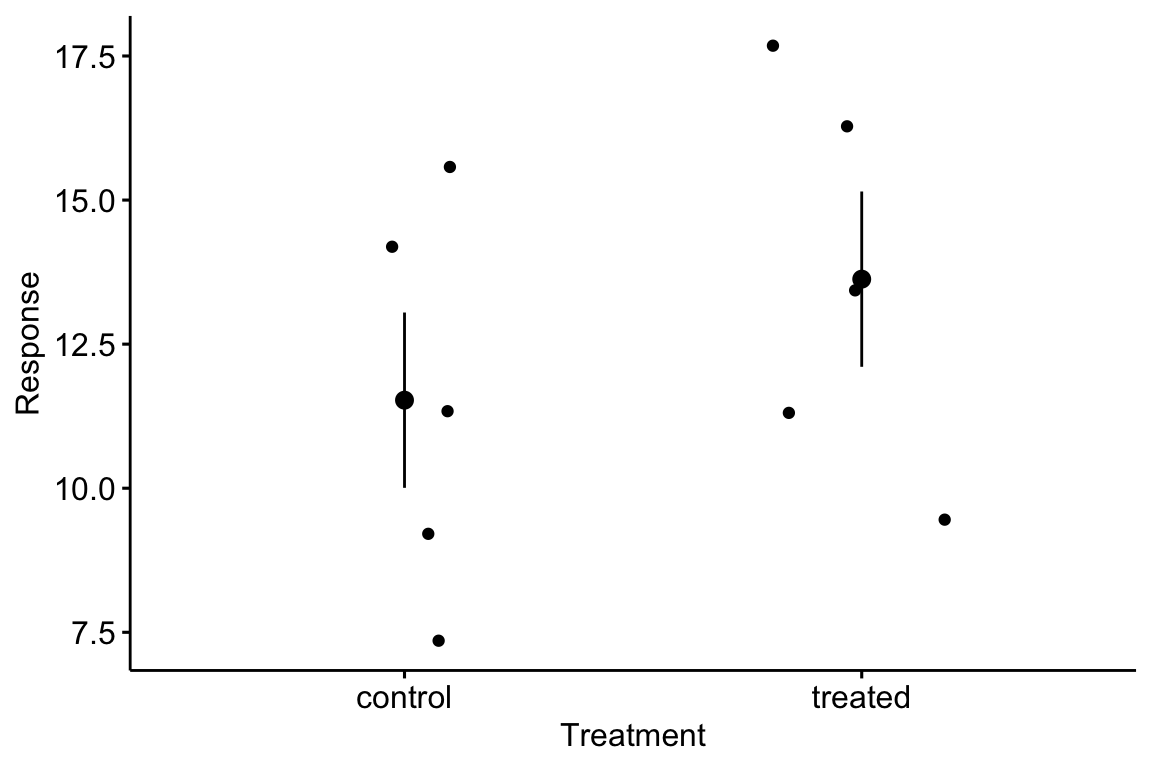
\includegraphics{Walker-elementary-statistical-modeling-draft_files/figure-latex/categorical-X-1.pdf}

\begin{Shaded}
\begin{Highlighting}[]
\CommentTok{# fit using base R linear model function}
\NormalTok{fit <-}\StringTok{ }\KeywordTok{lm}\NormalTok{(Response }\OperatorTok{~}\StringTok{ }\NormalTok{Treatment, }\DataTypeTok{data=}\NormalTok{fake_data)}
\CommentTok{# display a pretty table of the coefficients}
\NormalTok{knitr}\OperatorTok{::}\KeywordTok{kable}\NormalTok{(}\KeywordTok{coefficients}\NormalTok{(}\KeywordTok{summary}\NormalTok{(fit)), }\DataTypeTok{digits=}\DecValTok{3}\NormalTok{)}
\end{Highlighting}
\end{Shaded}

\begin{tabular}{l|r|r|r|r}
\hline
  & Estimate & Std. Error & t value & Pr(>|t|)\\
\hline
(Intercept) & 11.528 & 1.521 & 7.579 & 0.000\\
\hline
Treatmenttreated & 2.100 & 2.151 & 0.976 & 0.358\\
\hline
\end{tabular}

Check that the intercept is close to beta\_0 and the coefficient for
Treatment is close to beta\_1. This coefficient is the different in
means between the treatment levels. It is the simulated effect. Again,
change \(n\). Good values are \(n=20\) and \(n=100\). Again, comment out
the plot line to make exploration more efficient.

\section{Saving Data}\label{saving-data}

Let's save the fake data to the ``Fake\_Data'' folder. In the ``output''
folder create a new folder named ``week 01''. Then set the path to the
output folder:

\begin{Shaded}
\begin{Highlighting}[]
\NormalTok{output_path <-}\StringTok{ "../output"} \CommentTok{# out to parent directory than down into Fake_data}
\end{Highlighting}
\end{Shaded}

This could be done at the beginning of the notebook, especially if many
output files are saved. Regardless, now complete the file\_path with the
specifics of this save.

\begin{Shaded}
\begin{Highlighting}[]
\NormalTok{data_folder <-}\StringTok{ "week 01"}
\NormalTok{filename <-}\StringTok{ "my_first_fake_data.txt"}
\NormalTok{file_path <-}\StringTok{ }\KeywordTok{paste}\NormalTok{(output_path, data_folder, filename, }\DataTypeTok{sep=}\StringTok{"/"}\NormalTok{)}
\KeywordTok{write.table}\NormalTok{(fake_data, file_path, }\DataTypeTok{sep=}\StringTok{"}\CharTok{\textbackslash{}t}\StringTok{"}\NormalTok{, }\DataTypeTok{quote=}\OtherTok{FALSE}\NormalTok{)}
\end{Highlighting}
\end{Shaded}

We used \texttt{write.table()} to create a tab-delimited text file using
\texttt{sep="\textbackslash{}t"} to specify tabs to separate the row
elements. ``\t'' is the standard character string for a tab. Check in
your Fake\_Data folder and open the file in a text editor.

\section{Problems}\label{problems}

\begin{enumerate}
\def\labelenumi{\arabic{enumi}.}
\item
  Download the dataset ``data-Lodjak.et.al-2016-FuncEcol.xlsx'' from the
  Dryad repository at
  \url{https://datadryad.org/resource/doi:10.5061/dryad.rd01s}. The
  .xlsx file presents the data cleanly but the trade-off is that the 1)
  multiple header rows, and 2) spaces in the header labels, 3)
  parentheses in the header labels make it more complex to import in a
  usable way. Import the data and plot Body Mass against Age (that is
  make Body Mass the ``Y'' variable and Age the ``X'' variable) using
  the qplot function. You should recode the column labels to remove
  spaces and parentheses using the setnames function.
\item
  Download the dataset ``Results2015.txt'' from the Dryad repository at
  \url{https://datadryad.org//resource/doi:10.5061/dryad.65vk4}. Try to
  reproduce Fig. 1. It's not easy. I've inserted the figure below.
\item
  (grad students only) Download and plot data from a Dryad Repository
  dataset of your choice.
\item
  (grad students only) Create fake experimental data with three
  treatment levels (control, lo\_temp, high\_temp). This will require
  three parameters: an intercept (beta\_0), an effect of lo\_temp
  (beta\_1), and an effect of high\_temp (beta\_2). You should be able
  to plug and play from the script above even if you don't underdstand
  at this point what any of it is! Plot it as a strip chart, as above.
\end{enumerate}

\begin{figure}
\centering
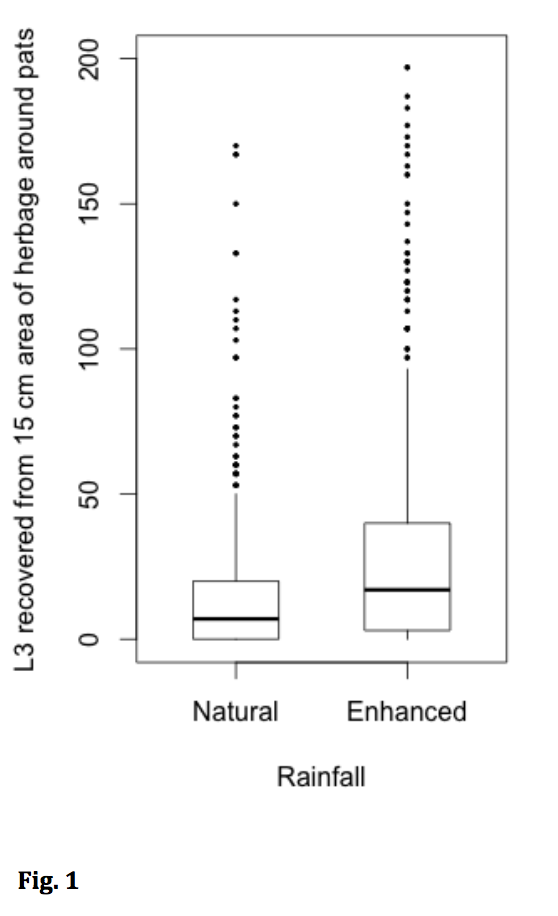
\includegraphics[width=0.50000\textwidth]{images/Dung_beetles_reduce_livestock-fig_1.png}
\caption{Fig. 1 from ``Dung beetles reduce livestock\ldots{}''}
\end{figure}

\chapter{Variability and Uncertainty (Standard Deviations and Standard
Errors)}\label{variability-and-uncertainty-standard-deviations-and-standard-errors}

\textbf{Uncertainty} is the stuff of science. A major goal of statistics
is measuring uncertainty. What do we mean by uncertainty? Uncertainty is
the error in estimating a parameter, such as the mean of a sample, or
the difference in means between two experimental treatments, or the
predicted response given a certain change in conditions. Uncertainty is
measured with a \textbf{variance} or its square root, which is a
\textbf{standard deviation}. The standard deviation of a statistic is
also (and more commonly) called a \textbf{standard error}.

Uncertainty emerges because of variability. In any introductory
statistics class, students are introduced to two measures of
variability, the ``standard deviation'' and the ``standard error.''
These terms are absolutely fundamental to statistics -- they are the
start of everything else. Yet, many biology professors confuse these
terms and certainly, introductory students do too.

When a research biologist uses the term ``standard deviation,'' they are
probably referring to the sample standard deviation which is a measure
of the variability of a sample. When a research biologist uses the term
``standard error,'' they are probably referring to the standard error of
a mean, but it could be the standard error of another statistics, such
as a regression slope. An important point to remember and understand is
that all standard errors \emph{are} standard deviations. This will make
more sense soon.

\section{The sample standard deviation vs.~the standard error of the
mean}\label{the-sample-standard-deviation-vs.the-standard-error-of-the-mean}

\subsection{Sample standard deviation}\label{sample-standard-deviation}

The sample standard deviation is a measure of the variability of a
sample. For example, were we to look at a histological section of
skeletal muscle we would see that the diameter of the fibers (the muscle
cells) is variable. We could use imaging software to measure the
diameter of a sample of 100 cells and get a \textbf{distribution} like
this

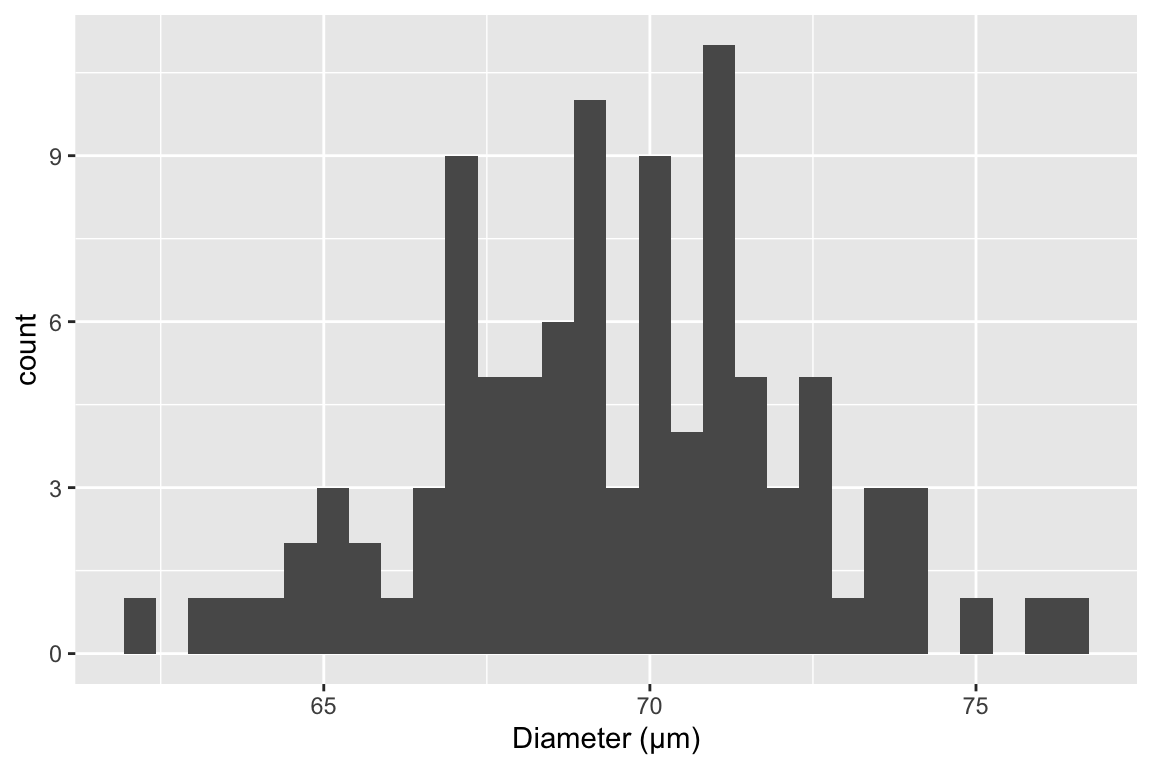
\includegraphics{Walker-elementary-statistical-modeling-draft_files/figure-latex/histogram-1.pdf}

The mean of this sample is 69.4 and the standard deviation is 2.8. The
standard deviation is the square root of the variance, and so computed
by

\begin{equation}
s_y = \sqrt{\frac{\sum_{i=1}^n{(y_i - \overline{y})^2}}{n-1}}
\label{eq:variance}
\end{equation}

Memorize this equation. To understand the logic of this measure of
variability, note that \(y_i - \overline{y}\) is the \textbf{deviation}
of the \(i\)th value from the sample mean, so the numerator is the sum
of squared deviations. The numerator is a sum over \(n\) items and the
denominator is \(n-1\) so the variance is (almost!) an averaged squared
deviation. More variable samples will have bigger deviations and,
therefore, bigger average squared deviations. Since the standard
deviation is the square root of the variance, a standard deviation is
the square root of an average squared deviation. This makes it similar
in value to the averaged deviation (or average of the absolute values of
the deviations since the average deviation is, by definition of a mean,
zero).

Notes on the variance and standard deviation

\begin{enumerate}
\def\labelenumi{\arabic{enumi}.}
\tightlist
\item
  Variances are additive but standard deviations are not. This means
  that the variance of the sum of two independent (uncorrelated) random
  variables is simply the sum of the variances of each of the variables.
  This is important for many statistical analyses.
\item
  The units of variance are the square of the original units, which is
  awkward for interpretation. The units of a standard deviation is the
  same as that of the original variable, and so is much easier to
  interpet.
\item
  For variables that are approximately normally distributed, we can map
  the standard deviation to the quantiles of the distribution. For
  example, 68\% of the values are within one standard deviation of the
  mean, 95\% of the values are within two standard deviations, and 99\%
  of the values are within three standard deviations.
\end{enumerate}

\subsection{Standard error of the
mean}\label{standard-error-of-the-mean}

A standard error of a statistic is a measure of the precision of the
statistic. The standard error of the mean is a measure of the precision
of the estimate of the mean. The smaller the standard error, the more
precise the estimate. The standard error of the mean (SEM) is computed
as

\begin{equation}
SEM = \frac{s_y}{\sqrt{n}}
\label{eq:se}
\end{equation}

The SEM is often denoted \(s_{\bar{y}}\) to indicate that it is a
standard deviation of the mean (\(\bar{y}\)). In what sense is a
standard error a measure of variability? This is kinda weird. If we
sample 100 cells in the slide of muscle tissue and compute the mean
diameter, how can the mean have a standard deviation? There is only one
value! To understand how the SEM is a standard deviation, imagine 1)
resampling 100 cells and 2) recomputing a mean from the re-sampled data
an infinite number of times and each time, you write down the newly
computed mean. The true standard error of the mean is the standard
deviation of this infinitely long column of means. This means that a
standard error of the mean, computed from a single sample using equation
\eqref{eq:se} is itself a sample statistic.

Notes on standard errors

\begin{enumerate}
\def\labelenumi{\arabic{enumi}.}
\tightlist
\item
  The SEM is only one kind of standard error. A standard deviation can
  be computed for any statistic -- these are all standard errors. For
  some statistics, such as the mean, the standard error can be computed
  directly using an equation, such as that for the SEM (equation
  \eqref{eq:se}. For other statistics, a computer intensive method such as
  the \textbf{bootstrap} is necessary to compute a standard error. We
  will return to the bootstrap at the end of this chapter.
\item
  The units of a standard error are the units of the measured variable.
\item
  A standard error is proportional to sample variability (the sample
  standard deviation, \(s_y\)) and inversely proportional to sample size
  (\(n\)). Sample variability is a function of both natural variation
  (there really is variation in diameter among fibers in the quadriceps
  muscle) and measurement error (imaging software with higher resolution
  can measure a diameter with less error). Since the SEM is a measure of
  the precision of estimating a mean, this means this precision will
  increase (or the SEM will decrease) if 1) an investigator uses methods
  that reduce measurement error and 2) an investigator computes the mean
  from a larger sample.
\item
  This last point (the SEM decreases with sample size) seems obvious
  when looking at equation \eqref{eq:se}, since \(n\) is in the
  denominator. Of course \(n\) is also in the denominator of equation
  \eqref{eq:variance} for the sample standard deviation but the standard
  deviation does not decrease as sample size increases. First this
  wouldn't make any sense -- variability is variability. A sample of
  10,000 cell diameters should be no more variable than a sample of 100
  cell diameters (think about if you agree with this or not). Second,
  this should also be obvious from equation \eqref{eq:variance}. The
  standard deviation is the square root of an average and averages don't
  increase with the number of things summed since both the the numerator
  (a sum) and denominator increase with \(n\).
\end{enumerate}

\section{Using Google Sheets to generate fake data to explore
uncertainty}\label{using-google-sheets-to-generate-fake-data-to-explore-uncertainty}

In statistics we are interested in estimated parameters of a
\textbf{population} using measures from a \textbf{sample}. The goal in
this section is to use Google Sheets (or Microsoft Excel) to use fake
data to discover the behavior of sampling and to gain some intuition
about uncertainty using standard errors.

\subsection{Steps}\label{steps}

\begin{enumerate}
\def\labelenumi{\arabic{enumi}.}
\tightlist
\item
  Open Google Sheets
\item
  In cell A1 type ``mu''. mu is the greek letter \(\mu\) and is very
  common notation for the poplation value (the TRUE value!) of the mean
  of some hypothetical measure. In cell B1, insert some number as the
  value of \(\mu\). Any number! It can be negative or positive.
\item
  In cell A2 type ``sigma''. sigma is the greek letter \(\sigma\).
  \(\sigma^2\) is very common (universal!) notation for the population
  (TRUE) variance of some measure or parameter. Notice that the true
  (population) values of the mean and variance are greek letters. This
  is pretty standard in statistics. In cell B2, insert some positive
  number (standard deviations are the positive square roots of the
  variance).
\item
  In cell A8 type the number 1
\item
  In cell A9 insert the equation ``=A8 + 1''. What is this equation
  doing? It is adding the number 1 to to the value in the cell above, so
  the resulting value should be 2.
\item
  In Cell B8, insert the equation ``=normsinv(rand())*\$B\$2 + \$B\$1``.
  The first part of the equation creates a random normal variable with
  mean 0 and standard deviation 1. multiplication and addition transform
  this to a random normal variable with mean \(\mu\) and standard
  deviation \(\sigma\) (the values you set in cells B1 and B2).
\item
  copy cell B8 and paste into cell B9. Now Higlight cells A9:B9 and copy
  the equations down to row 107. You now have 100 random variables
  sampled from a infinite population with mean \(\mu\) and standard
  deviation \(\sigma\).
\item
  In cell A4 write ``mean 10''. In cell B4 insert the equation
  ``=average(B8:B17)''. The resulting value is the \textbf{sample mean}
  of the first 10 random variables you created. Is the mean close to
  \(\mu\)?
\item
  In cell A5 write ``sd 10''. In cell B5 insert the equation
  ``stdev(B8:B17)''. The result is the \textbf{sample standard
  deviation} of the first 10 random variables. Is this close to
  \(\sigma\)?
\item
  In cell A6 write ``mean 100''. In cell B6 insert the equation
  ``=average(B8:B107)''. The resulting value is the \textbf{sample mean}
  of the all 100 random variables you created. Is this mean closer to
  \(\mu\) than mean 10?
\item
  In cell A7 write ``sd 100''. In cell B7 insert the equation
  ``=stdev(B8:B107)''. The resulting value is the \textbf{sample
  standard deviation} of the all 100 random variables you created. Is
  this SD closer to \(\sigma\) than sd 10?
\end{enumerate}

The sample standard deviation is a measure of the variability of the
sample. The more spread out the sample (the further each value is from
the mean), the bigger the sample standard deviation. The sample standard
deviation is most often simply known as ``The'' standard deviation,
which is a bit misleading since there are many kinds of standard
deviations!

Remember that your computed mean and standard deviations are estimates
computed from a sample. They are estimates of the true values \(\mu\)
and \(\sigma\). Explore the behavior of the sample mean and standard
deviation by re-calculating the spreadsheet. In Excel, a spreadsheet is
re-calculated by simultaneously pressing the command and equal key. In
Google, command-R recalculates but is painfully slow. Instead, if using
Google Sheets, just type the number 1 into a blank cell, and the sheet
recalculates quickly. Do it again. And again.

Each time you re-calculate, a new set of random numbers are generated
and the new means and standard deviations are computed. Compare mean 10
and mean 100 each re-calculation. Notice that these estimates are
variable. They change with each re-calculation. How variable is mean 10
compared to mean 100? The variability of the estimate of the mean is a
measure of \textbf{uncertainty} in the estimate. Are we more uncertain
with mean 10 or with mean 100? This variability is measured by a
standard deviation. This \textbf{standard deviation of the mean} is also
called the \textbf{standard error of the mean}. Many researchers are
loose with terms and use ``The'' standard error to mean the standard
error of the mean, even though there are many kinds of standard errors.
In general, ``standard error''" is abbreviated as ``SE.'' Sometimes
``standard error of the mean'' is specifically abbreviated to ``SEM.''

The standard error of the mean is a measure of the precision in
estimating the mean. The smaller the value the more precise the
estimate. The standard error of the mean \emph{is} a standard deviation
of the mean. This is kinda weird. If we sample a population one time and
compute a mean, how can the mean have a standard deviation? There is
only one value! And we compute this value using the sample standard
deviation: \(SEM = \frac{SD}{\sqrt{N}}\). To understand how the SEM is a
standard deviation, Imagine recalculating the spread sheet an infinite
number of times and each time, you write down the newly computed mean.
The standard error of the mean is the standard deviation of this
infinitely long column of means.

\section{Using R to generate fake data to explore
uncertainty}\label{using-r-to-generate-fake-data-to-explore-uncertainty}

note that I use ``standard deviation'' to refer to the sample standard
deviation and ``standard error'' to refer to the standard error of the
mean (again, we can compute standard errors as a standard deviation of
any kind of estimate)

\subsection{part I}\label{part-i}

In the exercise above, you used Google Sheets to generate \(p\) columns
of fake data. Each column had \(n\) elements, so the matrix of fake data
was \(n \times m\) (it is standard in most fields to specify a matrix as
rows by columns). This is \emph{much} easier to do in R and how much
grows exponentially as the size of the matrix grows.

To start, we just generate a \(n \times p\) matrix of normal random
numbers.

\begin{Shaded}
\begin{Highlighting}[]
\CommentTok{# R script to gain some intuition about standard deviation (sd) and standard error (se)}
\CommentTok{# you will probably need to install ggplot2 using library(ggplot2) }
\NormalTok{n <-}\StringTok{ }\DecValTok{6} \CommentTok{# sample size}
\NormalTok{p <-}\StringTok{ }\DecValTok{100} \CommentTok{# number of columns of fake data to generate}
\NormalTok{fake_data <-}\StringTok{ }\KeywordTok{matrix}\NormalTok{(}\KeywordTok{rnorm}\NormalTok{(n}\OperatorTok{*}\NormalTok{p, }\DataTypeTok{mean=}\DecValTok{0}\NormalTok{, }\DataTypeTok{sd=}\DecValTok{1}\NormalTok{), }\DataTypeTok{nrow=}\NormalTok{n, }\DataTypeTok{ncol=}\NormalTok{p) }\CommentTok{# create a matrix}
\end{Highlighting}
\end{Shaded}

the 3rd line is the cool thing about R. In one line I'm creating a
dataset with \(n\) rows and \(p\) columns. Each column is a sample of
the standard normal distribution which by definition has mean zero and
standard deviation of 1. But, and this is important, any sample from
this distribution will not have exactly mean zero and standard deviation
of 1, because it's a sample, the mean and standard deviation will have
some small errror from the truth. The line has two parts to it: first
I'm using the function ``rnorm'' (for random normal) to create a vector
of n*m random, normal deviates (draws from the random normal
distribution) and then I'm organizing these into a matrix (using the
function ``matrix'')

To compute the vector of means, standard deviations, and standard errors
for each column of \texttt{fake\_data}, use the \texttt{apply()}
function.

\begin{Shaded}
\begin{Highlighting}[]
\NormalTok{means <-}\StringTok{ }\KeywordTok{apply}\NormalTok{(fake_data,}\DecValTok{2}\NormalTok{,mean) }\CommentTok{# the apply function is super useful}
\NormalTok{sds <-}\StringTok{ }\KeywordTok{apply}\NormalTok{(fake_data,}\DecValTok{2}\NormalTok{,sd)}
\NormalTok{sems <-}\StringTok{ }\NormalTok{sds}\OperatorTok{/}\KeywordTok{sqrt}\NormalTok{(n)}
\end{Highlighting}
\end{Shaded}

\texttt{apply()} is a workhorse in many R scripts. Learn it. Know it.
Live it.

The SEM is the standard deviation of the mean, so let's see if the
standard deviation of the means is close to the true standard error. We
sampled from a normal distribution with SD=1 so the true standard is

\begin{Shaded}
\begin{Highlighting}[]
\DecValTok{1}\OperatorTok{/}\KeywordTok{sqrt}\NormalTok{(n)}
\end{Highlighting}
\end{Shaded}

\begin{verbatim}
## [1] 0.4082483
\end{verbatim}

and the standard deviation of the \(p\) means is

\begin{Shaded}
\begin{Highlighting}[]
\KeywordTok{sd}\NormalTok{(means)}
\end{Highlighting}
\end{Shaded}

\begin{verbatim}
## [1] 0.3731974
\end{verbatim}

Questions

\begin{enumerate}
\def\labelenumi{\arabic{enumi}.}
\tightlist
\item
  how close is \texttt{sd(means)} to the true SE?
\item
  change p above to 1000. Now how close is sd(means) to the true SE?
\item
  change p above to 10,000. Now how close is sd(means) to the true SE?
\end{enumerate}

\subsection{part II - means}\label{part-ii---means}

This is a visualization of the spread, or variability, of the sampled
means

\begin{Shaded}
\begin{Highlighting}[]
\KeywordTok{qplot}\NormalTok{(means)}
\end{Highlighting}
\end{Shaded}

\begin{verbatim}
## `stat_bin()` using `bins = 30`. Pick better value with `binwidth`.
\end{verbatim}

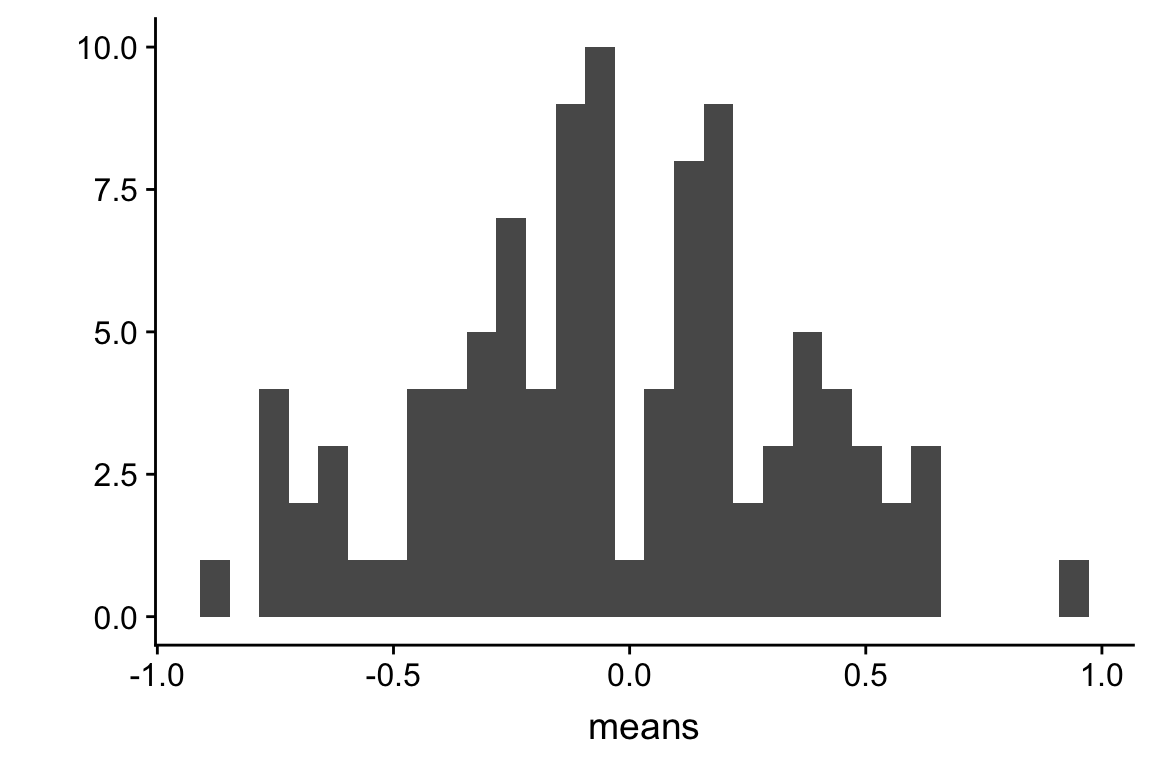
\includegraphics{Walker-elementary-statistical-modeling-draft_files/figure-latex/unnamed-chunk-6-1.pdf}

Compute the mean of the means

\begin{Shaded}
\begin{Highlighting}[]
\KeywordTok{mean}\NormalTok{(means)}
\end{Highlighting}
\end{Shaded}

\begin{verbatim}
## [1] -0.039961
\end{verbatim}

Questions

\begin{enumerate}
\def\labelenumi{\arabic{enumi}.}
\tightlist
\item
  Remember that the true mean is zero. How close, in general, are the
  sampled means to the true mean. How variable are the means? How is
  this quantified?
\item
  change n to 100, then replot. Are the means, in general, closer to the
  true mean? How variable are the means now?
\item
  Is the mean estimated with \(n=100\) closer to the truth, in general,
  then the mean estimated with \(n=6\)?
\item
  Redo with \(n=10000\)
\end{enumerate}

\subsection{part III - how do SD and SE change as sample size (n)
increases?}\label{part-iii---how-do-sd-and-se-change-as-sample-size-n-increases}

\begin{Shaded}
\begin{Highlighting}[]
\KeywordTok{mean}\NormalTok{(sds)}
\end{Highlighting}
\end{Shaded}

\begin{verbatim}
## [1] 1.017144
\end{verbatim}

Questions

\begin{enumerate}
\def\labelenumi{\arabic{enumi}.}
\tightlist
\item
  what is the mean of the standard deviations when n=6 (set p=1000)
\item
  what is the mean of the standard deviations when n=100 (set p=1000)
\item
  when n = 1000? (set p=1000)
\item
  when n = 10000? (set p=1000)
\item
  how does the mean of the standard deviations change as n increases
  (does it get smaller? or stay about the same size)
\item
  repeat the above with SEM
\end{enumerate}

\begin{Shaded}
\begin{Highlighting}[]
\KeywordTok{mean}\NormalTok{(sems)}
\end{Highlighting}
\end{Shaded}

\begin{verbatim}
## [1] 0.4152472
\end{verbatim}

Congratulations, you have just done a Monte Carlo simulation!

\subsection{\texorpdfstring{Part IV -- Generating fake data with ``for
loops''}{Part IV -- Generating fake data with for loops}}\label{part-iv-generating-fake-data-with-for-loops}

\begin{Shaded}
\begin{Highlighting}[]
\NormalTok{n <-}\StringTok{ }\DecValTok{6} \CommentTok{# sample size}
\NormalTok{n_iter <-}\StringTok{ }\DecValTok{10}\OperatorTok{^}\DecValTok{5} \CommentTok{# number of iterations of loop (equivalent to p)}
\NormalTok{means <-}\StringTok{ }\KeywordTok{numeric}\NormalTok{(n_iter)}
\NormalTok{sds <-}\StringTok{ }\KeywordTok{numeric}\NormalTok{(n_iter)}
\NormalTok{sems <-}\StringTok{ }\KeywordTok{numeric}\NormalTok{(n_iter)}
\ControlFlowTok{for}\NormalTok{(i }\ControlFlowTok{in} \DecValTok{1}\OperatorTok{:}\NormalTok{n_iter)\{}
\NormalTok{  y <-}\StringTok{ }\KeywordTok{rnorm}\NormalTok{(n) }\CommentTok{# mean=0 and sd=1 are default so not necessary to specify}
\NormalTok{  means[i] <-}\StringTok{ }\KeywordTok{mean}\NormalTok{(y)}
\NormalTok{  sds[i] <-}\StringTok{ }\KeywordTok{sd}\NormalTok{(y)}
\NormalTok{  sems[i] <-}\StringTok{ }\KeywordTok{sd}\NormalTok{(y)}\OperatorTok{/}\KeywordTok{sqrt}\NormalTok{(n)}
\NormalTok{\}}
\KeywordTok{sd}\NormalTok{(means)}
\end{Highlighting}
\end{Shaded}

\begin{verbatim}
## [1] 0.4090702
\end{verbatim}

\begin{Shaded}
\begin{Highlighting}[]
\KeywordTok{mean}\NormalTok{(sems)}
\end{Highlighting}
\end{Shaded}

\begin{verbatim}
## [1] 0.3883867
\end{verbatim}

Questions

\begin{enumerate}
\def\labelenumi{\arabic{enumi}.}
\tightlist
\item
  What do \texttt{sd(means)} and \texttt{mean(sems)} converge to as
  \texttt{n\_iter} is increased from 100 to 1000 to 10,000?
\item
  Do they converge to the same number?
\item
  Should they?
\item
  What is the correct number?
\end{enumerate}

Question number 4 is asking what is E(SEM), the ``expected standard
error of the mean''. There is a very easy formula to compute this. What
is it?

\section{Bootstrapped standard
errors}\label{bootstrapped-standard-errors}

The bootstrap is the best invention since duct tape. Really.

A standard error is the standard deviation of an infinite number of
hypothetically re-sampled means. A bootstrap standard error of a
statistic is the standard deviation of the statistic from a finite
number of resamples of the data! Wait what?

Let's download some data to explore this concept. The data are archived
at Dryad Repository.

\begin{enumerate}
\def\labelenumi{\arabic{enumi}.}
\tightlist
\item
  URL: \url{https://datadryad.org//resource/doi:10.5061/dryad.31cc4}
\item
  file: RSBL-2013-0432 vole data.xlsx
\item
  sheet: COLD VOLES LIFESPAN
\end{enumerate}

The data are the measured lifespans of the short-tailed field vole
(\emph{Microtus agrestis}) under three different experimental
treatments: vitamin E supplementation, vitamin C supplementation, and
control (no vitamin supplementation). Vitamins C and E are antioxidants,
which are thought to be protective of basic cell function since they
bind to the cell-damaging reactive oxygen species that result from cell
metabolism.

I've read in the file using read\_excel and converted to a data.table
named \texttt{vole}. I used \texttt{setnames} to rename the columns to
lifespan, control, vitamin\_E, and vitamin\_C. The data are in a
\textbf{wide format} -- that is instead of a single ``treatment''
column, there are three columns (``control'', ``vitamin C'', ``vitamin
E'') with value = 1, if that row (or lifespan) was assigned the
treatment of the column label and zero otherwise. In general, we want
data.tables to be in long format. Wide formats can be useful for some
computations but not really for these data.

Compute the standard error of the mean of the lifespan for the control
group using equation \eqref{eq:se}. One simple way to do this for the
control group is to extract the subset of the data satisfying the
condition control = 1 (the value in the column ``control'' equals 1). In
R, these conditional querries use \texttt{==}.

\begin{Shaded}
\begin{Highlighting}[]
\NormalTok{y <-}\StringTok{ }\KeywordTok{na.omit}\NormalTok{(vole[control}\OperatorTok{==}\DecValTok{1}\NormalTok{, lifespan]) }\CommentTok{# subset of data satisfying condition and omitting missing data, if these exist}
\NormalTok{n <-}\StringTok{ }\KeywordTok{length}\NormalTok{(y) }\CommentTok{# the sample size}
\NormalTok{se <-}\StringTok{ }\KeywordTok{sd}\NormalTok{(y)}\OperatorTok{/}\KeywordTok{sqrt}\NormalTok{(n}\OperatorTok{-}\DecValTok{1}\NormalTok{) }\CommentTok{# standard error of the mean}
\end{Highlighting}
\end{Shaded}

Okay, the SEM using equation \eqref{eq:se} is 31.9. Let's compare this
with a bootstrap estimate of the SEM.

\begin{Shaded}
\begin{Highlighting}[]
\NormalTok{n_iter <-}\StringTok{ }\DecValTok{2000} \CommentTok{# number of bootstrap iterations}
\NormalTok{means <-}\StringTok{ }\KeywordTok{numeric}\NormalTok{(n_iter) }\CommentTok{# we will save the means each iteration to this}
\NormalTok{inc <-}\StringTok{ }\DecValTok{1}\OperatorTok{:}\NormalTok{n }\CommentTok{# the first sample is the actual sample}
\ControlFlowTok{for}\NormalTok{(iter }\ControlFlowTok{in} \DecValTok{1}\OperatorTok{:}\NormalTok{n_iter)\{ }\CommentTok{# the for loop}
\NormalTok{  means[iter] <-}\StringTok{ }\KeywordTok{mean}\NormalTok{(y[inc])}
\NormalTok{  inc <-}\StringTok{ }\KeywordTok{sample}\NormalTok{(}\DecValTok{1}\OperatorTok{:}\NormalTok{n, }\DataTypeTok{replace=}\OtherTok{TRUE}\NormalTok{) }\CommentTok{# re-sample for the next iteration}
\NormalTok{\}}
\NormalTok{se_boot <-}\StringTok{ }\KeywordTok{sd}\NormalTok{(means)}

\CommentTok{#compare}
\NormalTok{se}
\end{Highlighting}
\end{Shaded}

\begin{verbatim}
## [1] 31.89536
\end{verbatim}

\begin{Shaded}
\begin{Highlighting}[]
\NormalTok{se_boot}
\end{Highlighting}
\end{Shaded}

\begin{verbatim}
## [1] 30.93843
\end{verbatim}

dayum!

\chapter{\texorpdfstring{A linear model with a single, continous
\emph{X}}{A linear model with a single, continous X}}\label{a-linear-model-with-a-single-continous-x}

\section{\texorpdfstring{A linear model with a single, continous
\emph{X} is classical
``regression''}{A linear model with a single, continous X is classical regression}}\label{a-linear-model-with-a-single-continous-x-is-classical-regression}

To introduce modeling with a single continous \(X\) variable, I'll use
data from

\begin{enumerate}
\def\labelenumi{\arabic{enumi}.}
\tightlist
\item
  Source: Dryad Digital Repository.
  \url{https://doi.org/10.5061/dryad.b3h4q}
\item
  File: ``FCM data dryad.csv''
\end{enumerate}

The data are from \citet{Dantzer_xxx}, who showed that North American
red squirrel (\emph{Tamiasciurus hudsonicus}) mothers from Yukon, Alaska
produce faster growing pups in years with increased squirrel density.
Remarkably, they even showed that perceived (but not actual) density
results in faster growing pups. To begin to investigate how pregnant
mothers control the future growth rate of pups, the researchers measured
the relationship between local squirrel density and the amount of fecal
cortisol metabolites from pregnant mothers. Cortisol is a hormone that
is secreted as part of stress response. The researchers were interested
in cortisol because it had previously been shownt that, in mammals,
blood cortisol levels in pregnant mothers have numerous effects on
offspring long past birth. If increased squirrel density causes
increased blood cortisol levels then we would expect to find a positive
relationship between \(Density\) and

\begin{figure}
\centering
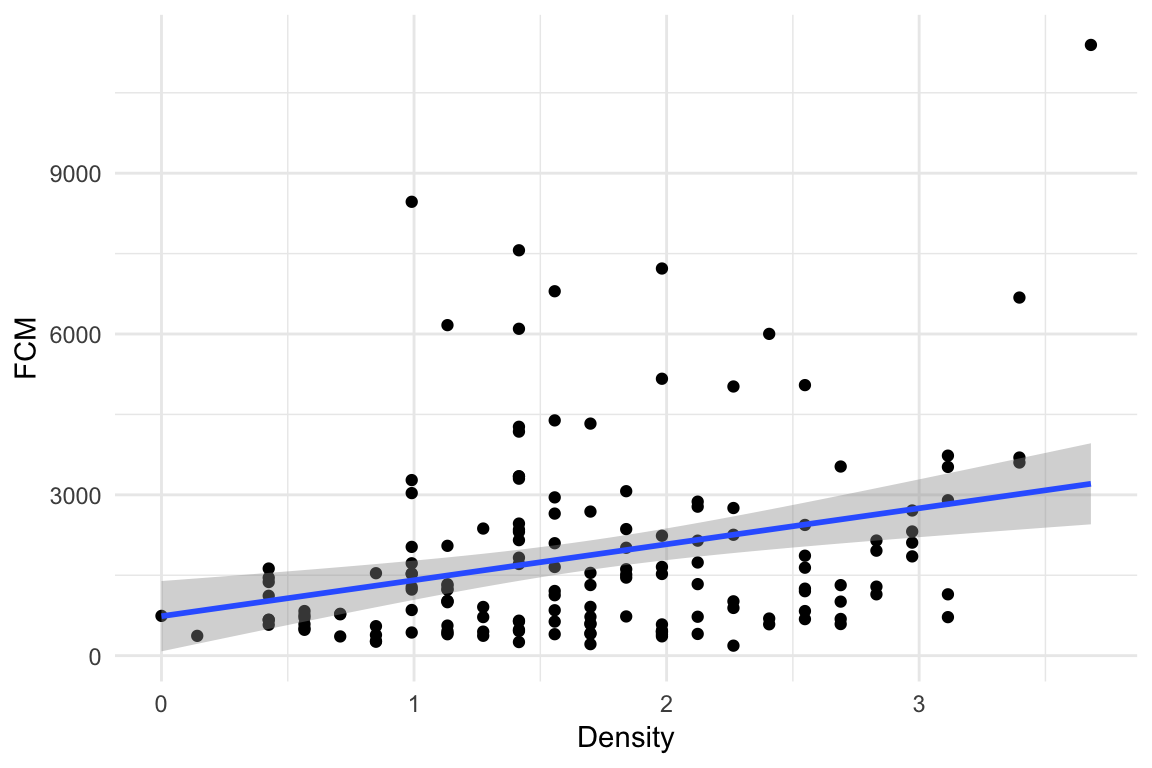
\includegraphics{Walker-elementary-statistical-modeling-draft_files/figure-latex/squirrel-1.pdf}
\caption{\label{fig:squirrel}A scatterplot of Fecal cortisol matabolites and
squirrel density.}
\end{figure}

Figure \ref{fig:squirrel} is a \textbf{scatterplot} of the data with the
amount of cortisol metabolites in the feces on the \(Y\) axis and local
squirrel density on the \(X\) axis. The line through the data is a
graphical representation of a linear model fit to the data and the gray
cloud around the line is a graphical representation of the uncertainty
in the model. The researchers wanted to model the ``effect'' of squirrel
density on the amount of cortisol metabolites in the feces of the
pregnant mothers. Graphically, this effect is the slope of the line in
Figure \ref{fig:squirrel}.

The model fit to the data is

\begin{equation}
FCM_i = \beta_0 + \beta_1 Density_i + \varepsilon_i
\label{eq:fcm-model}
\end{equation}

which contains both the linear predictor and the error. For inference,
for example, computing standard errors of the coefficients, We need to
model the error. Here, we use the simplest model of error which is ``IID
\(N(0, \sigma)\)''. This means, the modeled error is

\begin{enumerate}
\def\labelenumi{\arabic{enumi}.}
\tightlist
\item
  Independent -- individual error values are independent of other
  values.
\item
  Identical -- individual error can be thought of as a sample from a
  single \textbf{random distribution} (the same for each individual
  value). For this model, this distribution is
\item
  \(N(0, \sigma)\) -- the modeled distribution is ``Normal'' or
  ``Gaussian'', with a mean of zero and a standard deviation of
  \(\sigma\).
\end{enumerate}

The predictor part of the model is

\begin{equation}
\textrm{E}[FCM|Density] = \beta_0 + \beta_1 Density
\label{eq:regression}
\end{equation}

In words, model \eqref{eq:regression} reads ``the expected value of
\(FCM\) conditional on density is beta-knot plus beta-one times
density''. An \textbf{expected value} is a long run average -- if we
were to sample lots and lots of red squirrel populations with
\(Density=x\) (where \(x\) is a specific value), we'd expect the average
\(FCM\) across these samples to be \(\beta_0 + \beta_1 x\).

\begin{quote}
Let's unpack this. \(\textrm{E}[Y]\) is the \textbf{expectation} or
\textbf{expected value} of \(Y\). An expection is the long-run average
of \(Y\) if we were to run an experiment or re-sample a population many
times. The sample mean of \(Y\) is an estimate of \(\textrm{E}[Y]\).
\(\textrm{E}[Y|X]\) is a conditional expectation of \(Y\) -- it is the
expectation given additional conditions. Using the red squirrel example,
these conditions are a specific value of \(Density\). If \(FCM\) is
linearly related to \(Density\) (the right-hand side of equation
\eqref{eq:regression}) then the expected value of \(FCM\) given a local
density of 2.8 squirrels differs from the expected value of \(FCM\)
given a local density of 1.4 squirrels (the units of \(Density\) are
squirrels per 150 meter radius of the individual female's midden).
\end{quote}

In model \eqref{eq:regression}, there is a single \(X\) variable
(\(FCM\)). While the \(X\) variables are often called the ``dependent''
variables, in this model \(FCM\) does not ``depend'' on the independent
variable \(Density\) in any causal sense -- meaning if I were to
intervene and set \(Density\) to some value \(x\), I would expect
\(FCM\) to equal \(\beta_0 + \beta_1 x\). Rather, \(FCM\) only
``depends'' on \(Density\) in a probablistic sense -- if \(Density = x\)
then the most probable value of \(FCM\) is \(\beta_0 + \beta_1 x\). With
some strong assumptions model \eqref{eq:regression} can be turned into a
model of causal dependency, which is the focus of chapter xxx.

\(\beta_0\) and \(\beta_1\) are the \textbf{parameters} of model
\eqref{eq:regression}. Specifically \(\beta_0\) is the model
\textbf{intercept} and \(\beta_1\) is the modeled \textbf{effect} of
\(Density\). Again, the effect (\(\beta_1\)) has a probabilistic, and
not causal, interpretation. This interpretation is

\begin{equation}
\beta_1 = \textrm{E}[FCM|Density=x+1] - \textrm{E}[FCM|Density=x] 
\label{eq:beta1}
\end{equation}

Or, in words, ``beta-1 is the expected value of FCM when density equals
x + 1 minus the expected value of FCM when the density equals x.''
\(\beta_1\) is simply the difference in expected values given a one unit
difference in \(Density\). A very short way to state this is
``\(\beta_1\) is a difference in conditional means''.

\subsection{Using a linear model to estimate explanatory
effects}\label{using-a-linear-model-to-estimate-explanatory-effects}

The goal of the statistical model here is to estimate \(\beta_1\) -- the
probabalistic effect of \(Density\) on \(FCM\). This estimate, and a
measure of the uncertainty of this estimate, are in the table of
coefficients of the fit model

\begin{tabular}{l|r|r|r|r}
\hline
  & Estimate & Std. Error & t value & Pr(>|t|)\\
\hline
(Intercept) & 736.0 & 331.9 & 2.2 & 0.0281\\
\hline
Density & 671.1 & 178.9 & 3.8 & 0.0002\\
\hline
\end{tabular}

where the entries in the column ``Estimate'' are estimates of the
parameters \(\beta_0\) and \(\beta_1\) in model \eqref{eq:regression}. The
entries in the column ``Std. Error'' are the standard errors (SE) of the
estimates, which are measures of the uncertainty of the estimates.

The parameter estimates in the table above are the coefficients of the
fitted model

\begin{equation}
FCM_i = b_0 + b_1 Density_i + e_i
\label{eq:fcmi}
\end{equation}

where the subscript \emph{i} refers to the \emph{i}th individual. The
coefficients \(b_0\) and \(b_1\) are the y-intercept and the slope of
the line in Figure \ref{fig:squirrel}. The coefficient for \(Density\)
(\(b_1\)) is 671.1, and (given the definition of the parameter
\(\beta_1\) in equation \eqref{eq:beta1}) we expect squirrel mothers with
a local density of 2 squirrels within a 150 m radius of her midden to
average 671.1 more units of FCM (ng of fecal cortical metabolites per
gram dry food) than mother squirrels with a local density of only 1
squirrel within a 150 m radius of her midden.

\subsubsection{Probabilistic vs.~causal
conditioning}\label{probabilistic-vs.causal-conditioning}

Remember that this coefficient is estimating a probabilistic parameter.
Consequently, the coefficient \(b_1\) is simply a descriptor of a
pattern of relationship between local density and fecal cortisol
metabolites - no causal effect is implied. With the strong assumptions
explained in chapter xxx, however, \(b_1\) can estimate a causal effect.

\subsection{Using a linear model for
prediction}\label{using-a-linear-model-for-prediction}

Model \eqref{eq:fcmi} gives the measured value of \emph{FCM} for each
squirrel. The equation includes the linear predictor
(\(b_0 + b_1 Density_i\)) and the \textbf{residual} from the predictor
(\(e_i\)). The predictor part is called ``predictor'' because it is the
equation for predicting the value of an individual's \(FCM\) given that
individual's value of \(Density\):

\begin{equation}
\widehat{FCM} = b_0 + b_1 Density
\label{eq:fcmhat}
\end{equation}

where \(\widehat{FCM}\) is read as ``FCM hat'' and is the
\textbf{predicted value} or simply ``prediction''. Very often, we use
the predictor part (equation \eqref{eq:fcmhat}) to predict unknown or
future values given different modeled inputs (the \(X\)).

\subsection{Reporting results}\label{reporting-results}

The authors of the squirrel fcm data published a figure and table
similar to fig. xxx and table above but used a slightly more complex
linear model. Here is how the author's reported the results:

\begin{quote}
Across 6 years (2006 to 2011), we found a positive relationship between
local density and concentrations of fecal cortisol metabolites {[}FCM;
t\(_155\) = 3.63, P = 0.0002 (table S4 and Fig. 3A){]}.
\end{quote}

I would advocate reporting the estimate and a confidence interval
instead of \(t\) and \(p\). For example ``Across 6 years (2006 to 2011),
the probabilistic effect of local density on fecal cortisol metabolites
is 671.1 (95\% CI: 317.7, 1024.5). If a \(p\)-value is report \emph{in
addition} to the effect and CI, always report the exact \emph{p}-value,
which emphasizes the continuous nature of evidence against the null, and
not something like''\(p < 0.05\)``, which artificially dichotomizes the
evidence against the null.

\section{Working in R}\label{working-in-r}

\subsection{\texorpdfstring{Exploring the bivariate relationship between
\emph{Y} and
\emph{X}}{Exploring the bivariate relationship between Y and X}}\label{exploring-the-bivariate-relationship-between-y-and-x}

Questions

\begin{enumerate}
\def\labelenumi{\arabic{enumi}.}
\tightlist
\item
  Import the ``FCM data dryad.csv'' data from the Dryad repository as
  the data.table \texttt{fcm}
\item
  How are different words in the column labels demarcated? Is this good
  practice?
\end{enumerate}

Here we want to fit a model of \texttt{FCM.ng.g.dry} as a function of
\texttt{Raw.Squirrel.Density}. The authors used prior knowledge to
expect a positive relationship between these two variables. Use qplot to
generate a scatterplot of \(FCM\) against \(Density\)

Questions

\begin{enumerate}
\def\labelenumi{\arabic{enumi}.}
\setcounter{enumi}{2}
\tightlist
\item
  Is there a trend? If so, does the trend look linear or non-linear?
\item
  Does the residual variation (the deviation from the trend on the \(Y\)
  axis) look homogenous along the \(X\)-axis?
\item
  Are there any obvious outliers?
\end{enumerate}

\subsection{Fitting the linear model}\label{fitting-the-linear-model}

We will fit a linear model to the data using the \texttt{lm} function,
which is very general and will be our workhorse throughout the class.
The minimal input to the function is a model formula and the name of the
data.frame (remember, a data.table is a data.frame). A formula is of the
form \texttt{Y\ \textasciitilde{}\ X}. All of the output we assign to
the object \texttt{fit}.

Let's fit the linear model to the data using density as the predictor

\begin{Shaded}
\begin{Highlighting}[]
\NormalTok{  fit <-}\StringTok{ }\KeywordTok{lm}\NormalTok{(FCM.ng.g.dry }\OperatorTok{~}\StringTok{ }\NormalTok{Raw.Squirrel.Density, }\DataTypeTok{data=}\NormalTok{fcm)}
\end{Highlighting}
\end{Shaded}

R will look for the specified \(Y\) and \(X\) variables in the column
names of \texttt{fcm}. If these are not found, R will return an error,
for example

\begin{Shaded}
\begin{Highlighting}[]
\NormalTok{  fit <-}\StringTok{ }\KeywordTok{lm}\NormalTok{(FCM_ng_g_dry }\OperatorTok{~}\StringTok{ }\NormalTok{Raw_Squirrel_Density, }\DataTypeTok{data=}\NormalTok{fcm)}
\end{Highlighting}
\end{Shaded}

will return the error ``Error in eval(predvars, data, env) : object
`FCM\_ng\_g\_dry' not found''. This means your spelling and
capitalization have to be exact!

\subsection{\texorpdfstring{Getting to know the linear model: the
\texttt{summary}
function}{Getting to know the linear model: the summary function}}\label{getting-to-know-the-linear-model-the-summary-function}

The \texttt{lm} function returns an \texttt{lm} object, which we've
assigned to the name \texttt{fit}. \texttt{fit} contains lots of
information about our fit of the linear model to the data. Most of the
information that we want for most purposes can be retrieved with the
\texttt{summary} function, which is a general-purpose R command the
works with many R objects.

\begin{Shaded}
\begin{Highlighting}[]
\KeywordTok{summary}\NormalTok{(fit)}
\end{Highlighting}
\end{Shaded}

\begin{verbatim}
## 
## Call:
## lm(formula = FCM.ng.g.dry ~ Raw.Squirrel.Density, data = fcm)
## 
## Residuals:
##     Min      1Q  Median      3Q     Max 
## -2107.5 -1108.3  -434.9   511.8  8186.8 
## 
## Coefficients:
##                      Estimate Std. Error t value Pr(>|t|)    
## (Intercept)             736.0      331.9   2.217 0.028078 *  
## Raw.Squirrel.Density    671.1      178.9   3.752 0.000248 ***
## ---
## Signif. codes:  0 '***' 0.001 '**' 0.01 '*' 0.05 '.' 0.1 ' ' 1
## 
## Residual standard error: 1732 on 154 degrees of freedom
##   (7 observations deleted due to missingness)
## Multiple R-squared:  0.08374,    Adjusted R-squared:  0.07779 
## F-statistic: 14.07 on 1 and 154 DF,  p-value: 0.0002484
\end{verbatim}

What is here:

\textbf{Call}. This is the model that was fit

\textbf{Residuals}. This is a summary of the distribution of the
residuals. From this one can get a sense of the distribution (for
inference, the model assumes a normal distribution with mean zero). More
useful ways to examine this distribution will be introduced later in
this chapter.

\textbf{Coefficients table}. This contains the linear model coefficients
and their standard error and associated \(t\) and \(p\) values.

\begin{enumerate}
\def\labelenumi{\arabic{enumi}.}
\tightlist
\item
  The column of values under ``Estimate'' are the coefficients of the
  fitted model (equation \eqref{eq:fcmi}). Here, 735.9604344 is the
  intercept (\(b_0\)) and 671.1379749 is the effect of \(Density\)
  (\(b_1\)).
\item
  The column of values under ``Std. Error'' are the standard errors of
  the coefficients.
\item
  The column of values under ``t value'' are the \emph{t-statistics} for
  each coefficient. A \(t\)-value is a \textbf{signal to noise ratio}.
  The coefficient \(b_1\) is the ``signal'' and the SE is the noise. Get
  used to thinking about this ratio. Any \(t\) less than 2 is indicative
  of too much noise to say much about the signal. A \(t\) between 2 and
  3 means the noise is large enough to suggest an effect. A \(t\)
  greater than 3 is pretty good evidence of an effect.
\item
  The column of values under ``Pr(\textgreater{}\textbar{}t\textbar{})''
  is the \(p\)-value, which is the exact probability associated with a
  particular \(t\). What is the \(p\)-value a test of? The \(p\)-value
  tests the hypothesis ``how probable are the data if the coefficient is
  zero?''. Formally \(P = \mathrm{freq(t' \ge t|H_o)}\), where \(t'\) is
  the hypothetical t-value, t is the observed \(t\)-value, and \(H_o\)
  is the null hypothesis. We will return to \(p\)-values in Chapter xxx.
\end{enumerate}

\textbf{Signif. codes}. I am surprised that base R returns this. These
are useless because the concept of ``levels of significance'' is
muddled, as will be discussed in Chapter xxx.

Beneath the Signif. codes are some model statistics which are useful

\textbf{Residual standard error} This is \(\sqrt{\sum{e_i^2}/(n-2)}\),
where \(e_i\) are the residuals in the fitted model. ``degrees of
freedom'' is the number of \(e_i\) that are ``allowed to vary'' after
fitting the parameters, so is the total sample size (\(n\)) minus the
number of parameters fit. The fit model has two fit parameters (\(b_0\)
and \(b_1\) so the df is \(n-2\). Note that this is the denominator in
the residual standard error equation.

\textbf{Multiple R-squared}. This is an important but imperfect summary
measure of the whole model that effectively measures how much of the
total variance in the response variable ``is explained by'' the model.
Its value lies between zero and 1. \textbf{It's a good measure to report
in a manuscript}.

\textbf{F-statistic and p-value}. These are statistics for the whole
model (not the individual coefficients) and I just don't find these very
useful.

Note that the \(p\)-value for the coefficient for Raw.Squirrel.Density
is very small and we could conclude that the data are not consistant
with a model of no slope. But did we need a formal hypothesis test for
this? We haven't learned much if we have only learned that the slope is
``not likely to be exactly zero''. What we want to know is not \emph{if}
there is a relationship between \(FCM\) and \(Density\), which is
imperfectly answered with a \(p\)-value, but \emph{the sign and
magnitude} of the relationship and the uncertainty in this estimate. For
this, we don't need the \(p\)-value. Instead, we want to interpret the
coefficient to its SE directly (for a quick-and-dirty interpretation) or
the confidence interval of the effect (for a more formal
interpretation). Please read this paragraph again. We will come back to
it over and over.

\subsection{display: An alternative to
summary}\label{display-an-alternative-to-summary}

Much of what we want to know about a model fit is returned by the
\texttt{display} function from the \texttt{arm} package.

\begin{Shaded}
\begin{Highlighting}[]
\KeywordTok{display}\NormalTok{(fit)}
\end{Highlighting}
\end{Shaded}

\begin{verbatim}
## lm(formula = FCM.ng.g.dry ~ Raw.Squirrel.Density, data = fcm)
##                      coef.est coef.se
## (Intercept)          735.96   331.94 
## Raw.Squirrel.Density 671.14   178.90 
## ---
## n = 156, k = 2
## residual sd = 1732.02, R-Squared = 0.08
\end{verbatim}

The \texttt{display} function does not give a \(t\)-value or a
\(p\)-value of the coefficients because the authors of the arm package
do not think \(p\)-values are very valuable. We don't need a \(t\)
because one can mentally compute the approximate ratio of the
coefficient to its SE and get a sense of the signal to noise, and that's
all the authors of the display function think we need.

\subsection{Confidence intervals}\label{confidence-intervals}

Confidence intervals for the coefficients of the model are obtained by

\begin{Shaded}
\begin{Highlighting}[]
\KeywordTok{confint}\NormalTok{(fit)}
\end{Highlighting}
\end{Shaded}

\begin{verbatim}
##                          2.5 %   97.5 %
## (Intercept)           80.21785 1391.703
## Raw.Squirrel.Density 317.73057 1024.545
\end{verbatim}

\texttt{confint} returns by default the 95\% confidence interval (CI) of
all parameters. The most useful way of thinking about the meaning of a
CI is

\textbf{A confidence interval contains the range of parameter values
that are consistent with the data, in the sense that a \(t\)-test would
not reject the null hypothesis of a difference between the estimate and
any value within the interval}

A more textbook way of defining a CI is: A 95\% CI of a parameter has a
95\% probability of including the true value of the parameter. It does
not mean that there is a 95\% probability that the true value lies in
the interval. This is a subtle but important difference. Here is a way
of thinking about the proper meaning of the textbook definition: we
don't know the true value of \(\beta_1\) but we can 1) repeat the
experiment or sampling, 2) re-estimate \(\beta_1\), and 3) re-compute a
95\% CI. If we do 1-3 many times, 95\% of the CIs will include
\(\beta_1\) within the interval.

Confidence intervals are often interpreted like \(p\)-values. That is,
the researcher looks to see if the CI overlaps with zero and if it does,
concludes there is ``no effect''. First, this conclusion is not correct
-- \textbf{the inability to find sufficient evidence for an effect does
not mean there is no effect, it simply means there is insufficient
evidence to conclude there is an effect}!

Second, what we want to use the CI for is to guide us about how big or
small the effect might reasonably be, given the data. Again, A CI is a
measure of parameter values that are ``consistent'' with the data. If
our biological interpretations at the small-end and at the big-end of
the interval's range radically differ, then we don't have enough
\emph{precision} in our analysis to reach an unambiguous conclusion.
Remember this.

\subsection{How good is our model?}\label{how-good-is-our-model}

How well does variation in \(Density\) ``explain'' variation in \(FCM\)?
The answer to this is in the \(R^2\) value, which is given in
\texttt{display(fit)} and in \texttt{summary(fit)} and accessed directly
with

\begin{Shaded}
\begin{Highlighting}[]
\KeywordTok{summary}\NormalTok{(fit)}\OperatorTok{$}\NormalTok{r.squared}
\end{Highlighting}
\end{Shaded}

\begin{verbatim}
## [1] 0.08373756
\end{verbatim}

\(R^2\) is the fraction of the total variance of \(Y\) explained by the
model, or more specifically, the linear predictor. It will vary from
zero (the model explains nothing) to one (the model explains
everything). If \(R^2=0\) the response is completely unpredictable by
the predictors. We can think of the values of the response as white
noise or all error. This doesn't mean that the values are ``not caused''
or ``random'' or not predicted by some other variable. It only means the
values are random with respect to the \(X\) variable(s) in the model. If
\(R^2=1\) we can \emph{exactly} predict the response from the \(X\)
variables in the model. So the bigger the \(R^2\), the better the model
in the sense that the response is more predicatable. \textbf{Super
importantly}, ``explains'' is in a probabilistic and not causal sense.
We will explore this concept much more in future worksheets.

\subsection{Model checking}

\texttt{plot} is a very useful base R function for ``model checking'' or
``model diagnostics'' to see if our model fit is acceptable.

\begin{Shaded}
\begin{Highlighting}[]
\KeywordTok{plot}\NormalTok{(fit)}
\end{Highlighting}
\end{Shaded}

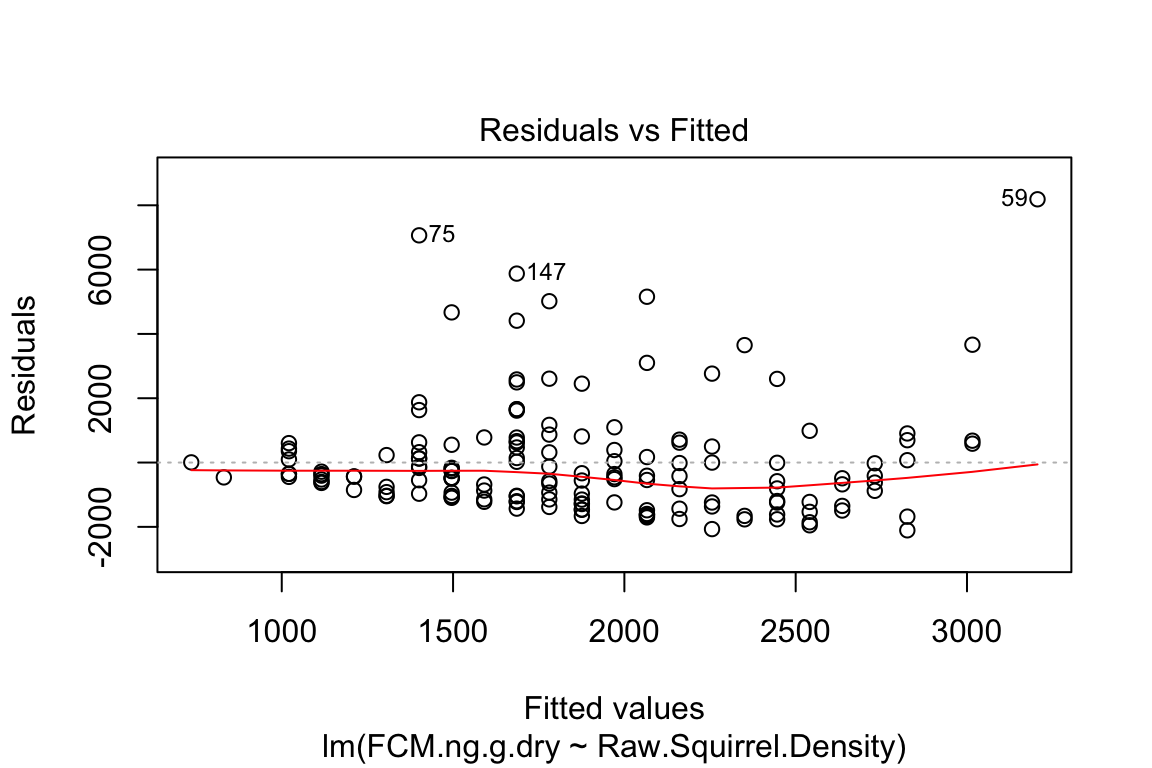
\includegraphics{Walker-elementary-statistical-modeling-draft_files/figure-latex/fit-diagnostics-1.pdf}
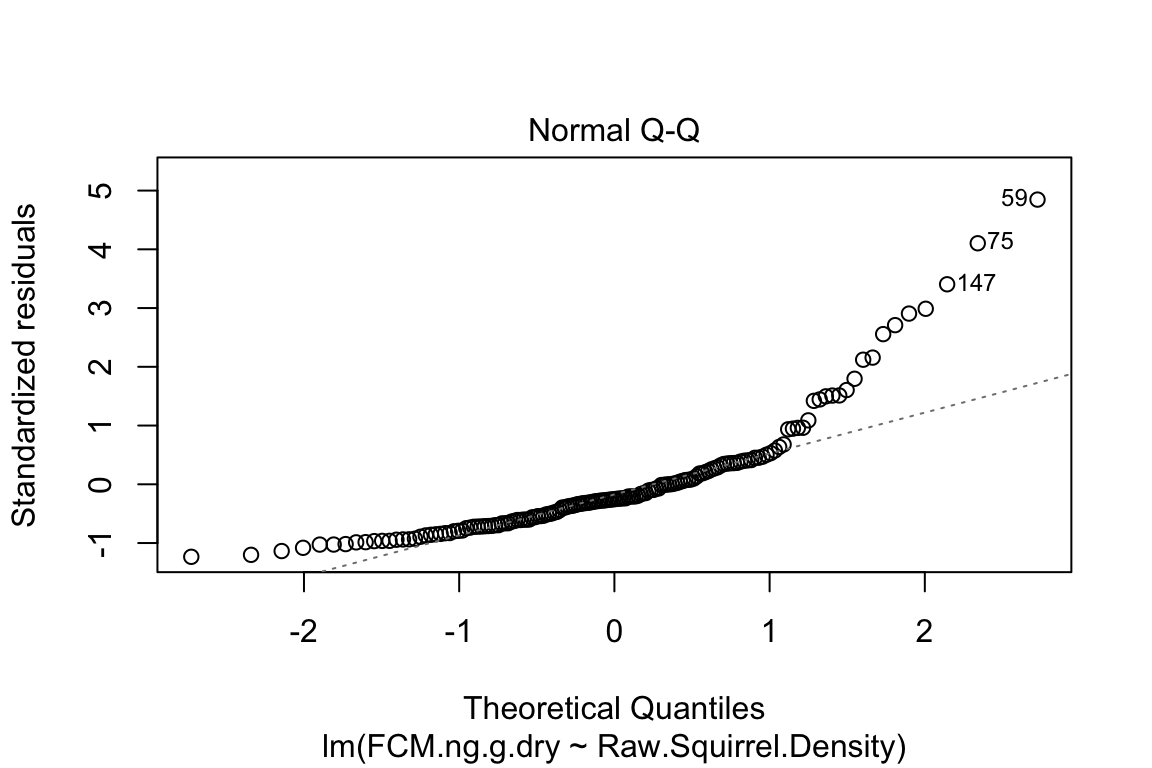
\includegraphics{Walker-elementary-statistical-modeling-draft_files/figure-latex/fit-diagnostics-2.pdf}
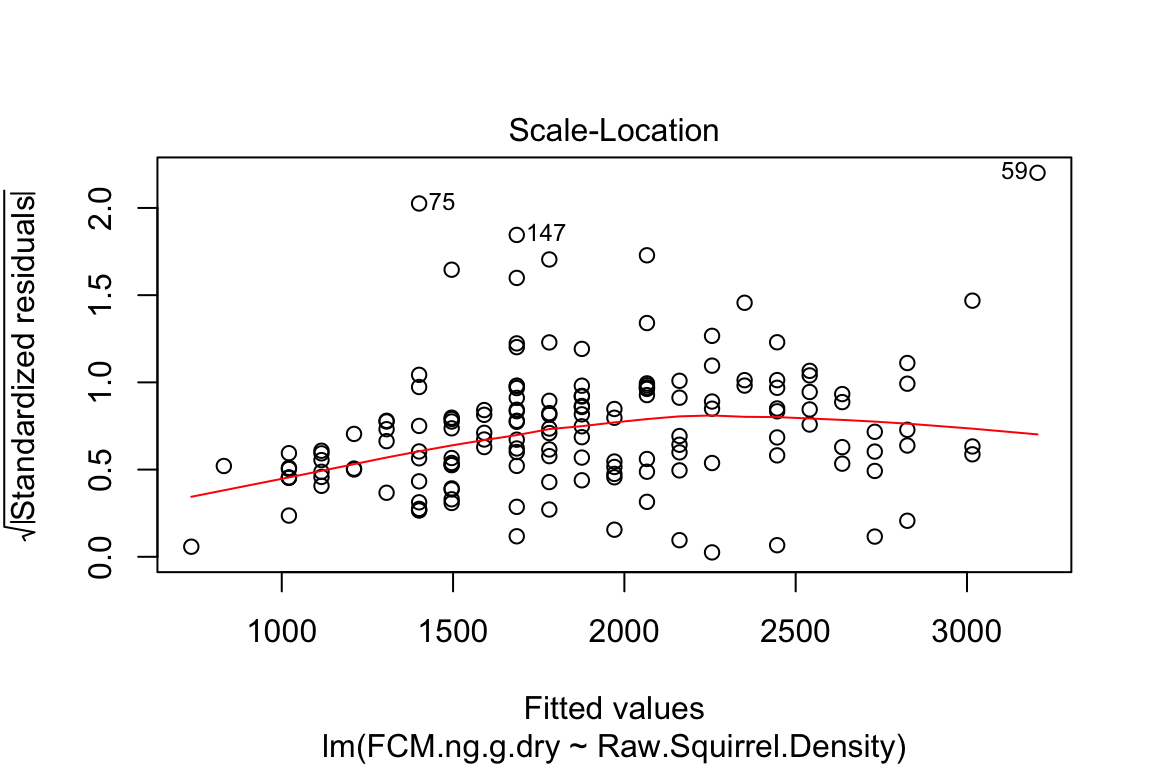
\includegraphics{Walker-elementary-statistical-modeling-draft_files/figure-latex/fit-diagnostics-3.pdf}
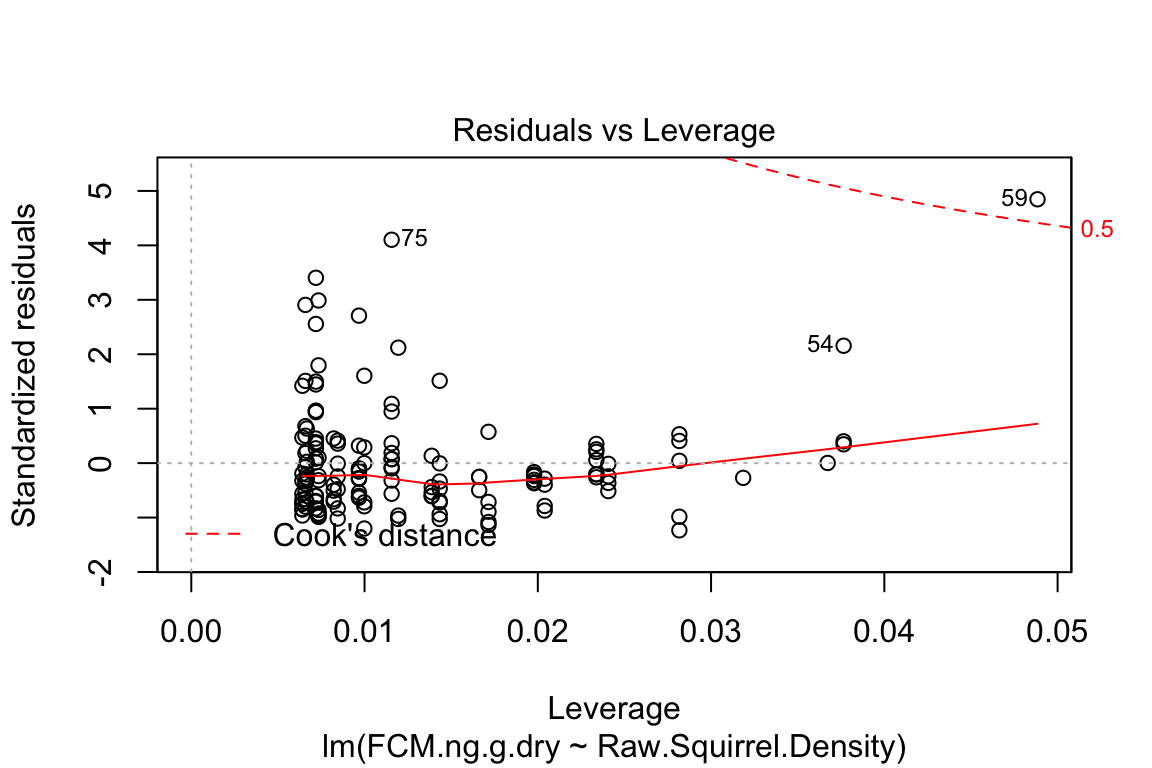
\includegraphics{Walker-elementary-statistical-modeling-draft_files/figure-latex/fit-diagnostics-4.pdf}

Compare the four diagnostic plots using the guidelines from here
\url{http://data.library.virginia.edu/diagnostic-plots/}

Questions

\begin{enumerate}
\def\labelenumi{\arabic{enumi}.}
\setcounter{enumi}{5}
\tightlist
\item
  Look at the plots you just made. What is a residual? What is a fitted
  value?
\end{enumerate}

\subsection{exploring a lm object}\label{exploring-a-lm-object}

\texttt{fit} contains much information but simply typing \texttt{fit}
into the console gives us only the model and the coefficients.
\texttt{names} is a super important R function. It gives us the names of
all the parts of some R object. \texttt{fit} is an lm object.
\texttt{names(fit)} gives us all the parts contained in an lm object.

\begin{Shaded}
\begin{Highlighting}[]
\KeywordTok{names}\NormalTok{(fit)}
\end{Highlighting}
\end{Shaded}

\begin{verbatim}
##  [1] "coefficients"  "residuals"     "effects"       "rank"         
##  [5] "fitted.values" "assign"        "qr"            "df.residual"  
##  [9] "na.action"     "xlevels"       "call"          "terms"        
## [13] "model"
\end{verbatim}

You can see any of these parts using the dollar sign

Questions

\begin{enumerate}
\def\labelenumi{\arabic{enumi}.}
\setcounter{enumi}{6}
\item
  What does \texttt{fit\$residuals} return? Answer using equation
  \eqref{eq:fcmi}
\item
  What does \texttt{fit\$fitted.values} return? Answer using equation
  @ref(eq:fcmi
\end{enumerate}

You can use qplot to make a plot similar to the first plot of
\texttt{plot(fit)}

\begin{Shaded}
\begin{Highlighting}[]
\KeywordTok{qplot}\NormalTok{(fit}\OperatorTok{$}\NormalTok{fitted.values, fit}\OperatorTok{$}\NormalTok{residuals, }\DataTypeTok{geom=}\KeywordTok{c}\NormalTok{(}\StringTok{'point'}\NormalTok{, }\StringTok{'smooth'}\NormalTok{))}
\end{Highlighting}
\end{Shaded}

\begin{verbatim}
## `geom_smooth()` using method = 'loess' and formula 'y ~ x'
\end{verbatim}

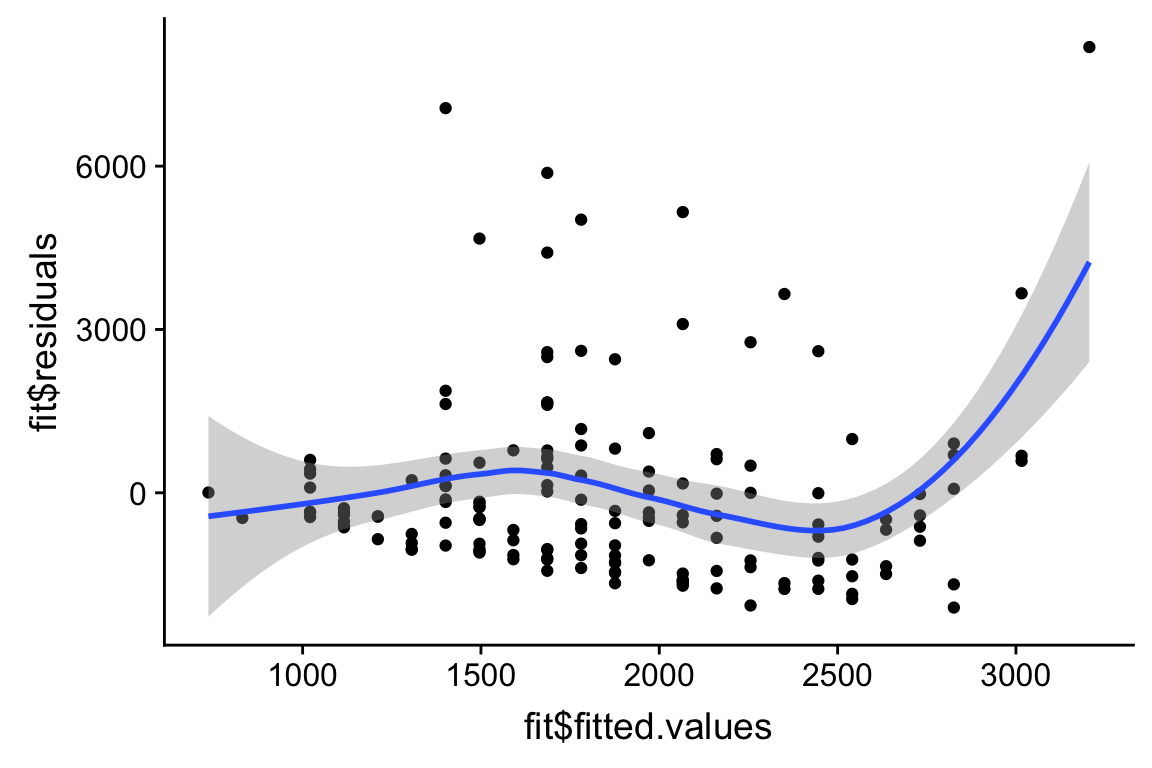
\includegraphics{Walker-elementary-statistical-modeling-draft_files/figure-latex/fit-fitted-1.pdf}

\section{Problems}\label{problems-1}

\begin{enumerate}
\def\labelenumi{\arabic{enumi}.}
\tightlist
\item
  Using the chick data from Chapter 3. Compare the effects of
  nest\_temperature\_above\_ambient on day13\_mass by fitting two
  separate linear models 1) one using only the control group and one
  using the treated group. The grouping variable is playback\_treatment.
  These models were plotted in Chapter 3 so \texttt{lm} will return the
  linear model behind these plots.
\end{enumerate}

Report the results using the two effect estimates and a 95\% confidence
interval (we will learn in a later chapter a more sophisticated way of
comparing the effects between the groups)

\textbf{file name}: ``allDatasetsMarietteBuchanan2016.xls''

\textbf{source}: \url{https://datadryad.org//handle/10255/dryad.122315}

\begin{enumerate}
\def\labelenumi{\arabic{enumi}.}
\setcounter{enumi}{1}
\tightlist
\item
  (Grad students only) -- find a dataset using Dryad that has data that
  can be fit by a simple linear model with a single continuous \(X\)
  (its okay if the authors fit the data with a more complex model). Fit
  the data and report the results with a plot and text.
\end{enumerate}

\chapter{Least Squares Estimation}\label{least-squares-estimation}

The linear models in the last chapter and for much of this book are fit
to data using a method called ``ordinary least squares'' (OLS). This
chapter explores the meaning of OLS and related statistics, including
\(R^2\), as well as some alternative methods for bivariate regression.

\section{OLS regression}\label{ols-regression}

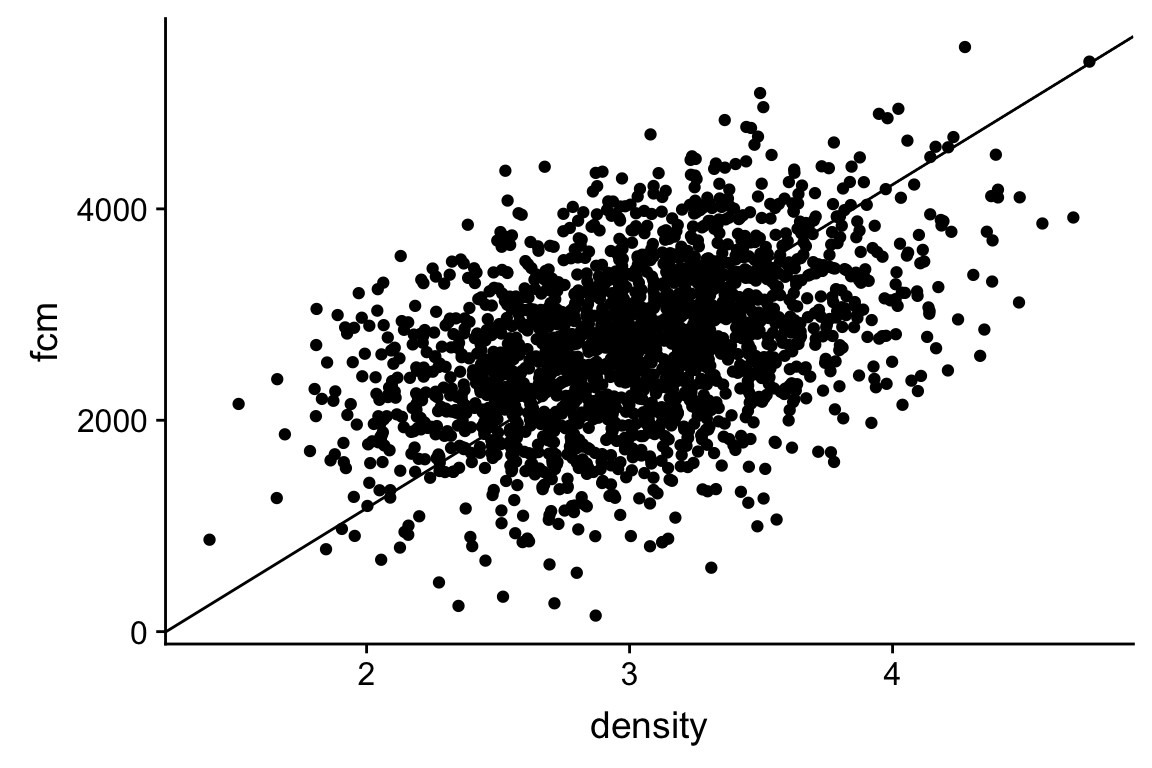
\includegraphics{Walker-elementary-statistical-modeling-draft_files/figure-latex/fake-data-ma-1.pdf}

The fake data illustrated in the scatterplot above (Figure
\ref{fig:fake-data-ma}) were modeled to look something like the squirrel
fecal cortisol metabolite data in the previous chapter. If a typical
student is asked to draw a regression line through the scatter, they
typically draw a line similar to that in Figure \ref{fig:fake-data-ma}.
This line is not the OLS regression line but the major axis of an elipse
that encloses the scatter of points--that students invariably draw this
line suggests that the brain interprets the major axis of an elliptical
scatter of points as a trend (This major axis line is an alternative
method for estimating a slope and is known as standard major-axis
regression. More about this at the end of this chapter.)

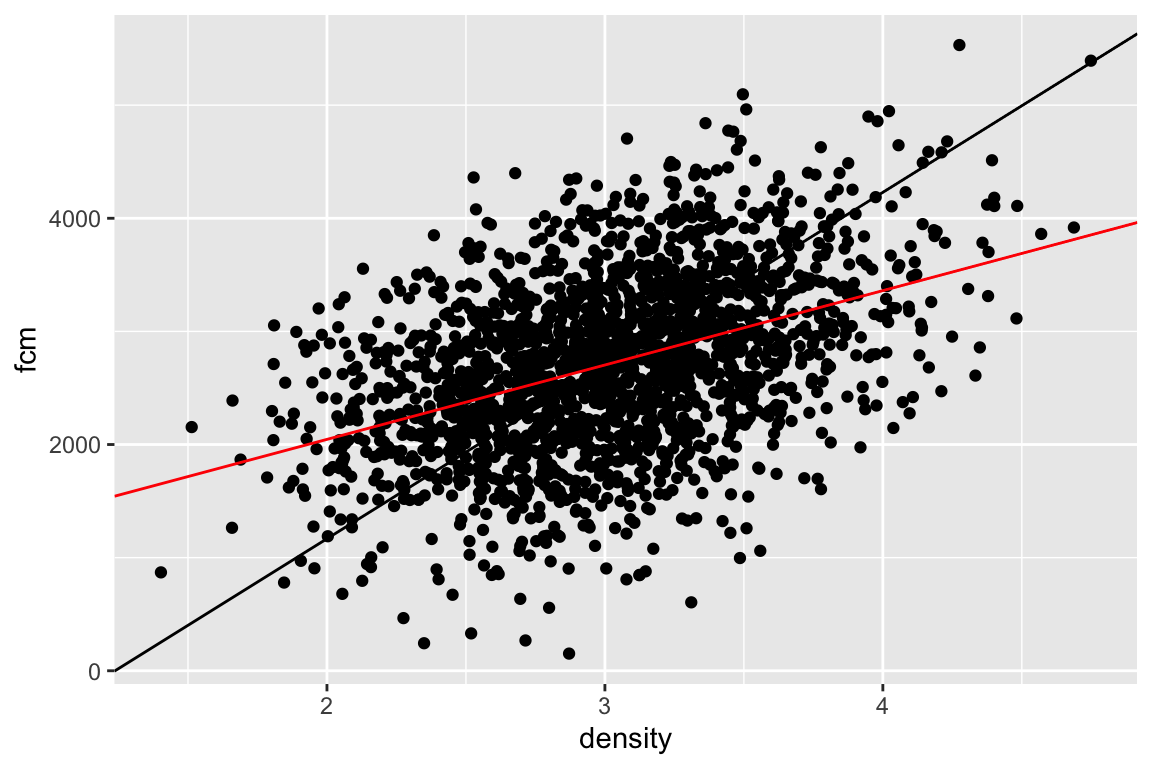
\includegraphics{Walker-elementary-statistical-modeling-draft_files/figure-latex/fake-data-ols-1.pdf}

The OLS regression line is the red line in Figure
\ref{fig:fake-data-ols} -- the standard major axis line is left for
comparison). The OLS regression line

\begin{enumerate}
\def\labelenumi{\arabic{enumi}.}
\tightlist
\item
  passes through the bivariate mean (\(\bar{x}\), \(\bar{y}\)) of the
  scatter, and
\item
  minimizes the sum of the squared deviations from each point to it's
  modeled value \(\sum{(y_i - \hat{y}_i)^2}\)
\end{enumerate}

There are an infinite number of lines that pass through the bivariate
mean (think of anchoring a line at the bivariate mean and spinning it).
The OLS line is the line that minimizes the squared (vertical)
deviations (``least squares'').

For a bivariate regression, the slope (coefficient \(b_1\) of \(X\)) of
the OLS model fit is computed by

\begin{equation}
b_1 = \frac{\mathrm{COV}(X, Y)}{\mathrm{VAR}(X)}
\end{equation}

This equation is worth memorizing. We will generalize this into a more
flexible equation in a few chapters.

\section{\texorpdfstring{How well does the model fit the data? \(R^2\)
and ``variance
explained''}{How well does the model fit the data? R\^{}2 and variance explained}}\label{how-well-does-the-model-fit-the-data-r2-and-variance-explained}

Let's switch to real data.

\begin{enumerate}
\def\labelenumi{\arabic{enumi}.}
\tightlist
\item
  Source: Dryad Digital Repository.
  \url{https://doi.org/10.5061/dryad.056r5}
\item
  File: ``Diet-shift data.xls''
\end{enumerate}

Fish require arachidonic acid (ARA) and other highyly unsaturated fatty
acids in their diet and embryo and yolk-stage larvae obtain these from
yolk. Fuiman and Faulk (xxx) designed an experiment to investigate if
red drum (\emph{Sciaenops ocellatus}) mothers provision the yolk with
ARA from recent dietary intake or from stored sources in somatic
tissues. The data below are from experiment 8. The \emph{x}-axis is the
days since a diet shift to more and less ARA (\(days\)) and the
\emph{y}-axis is the ARA content of the eggs (\(ARA\)).

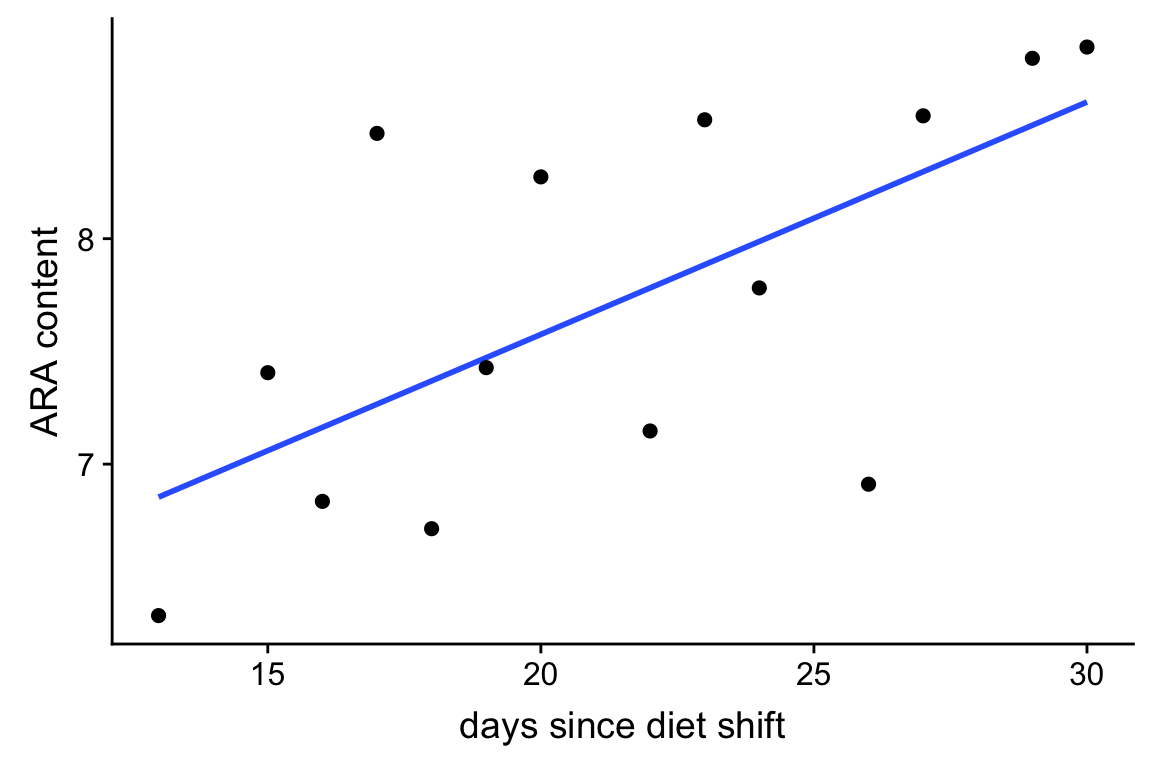
\includegraphics{Walker-elementary-statistical-modeling-draft_files/figure-latex/egg-data-1.pdf}

The statistic \(R^2\) is a measure of the fit of a model to data. The
\(R^2\) for the fit of the egg data is 0.42. \(R^2\) is the fraction of
two variances \(\frac{\mathrm{VAR}(Model)}{\mathrm{VAR}(Y)}\), or, the
fraction of the variance of \(Y\) ``explained by the model.'' The value
of \(R^2\) ranges from zero (the fit cannot be any worse) to one (the
fit is ``pefect'').

To understand \(R^2\), and its computation, a bit more, let's look at
three kinds of deviations.

\begin{figure}
\centering
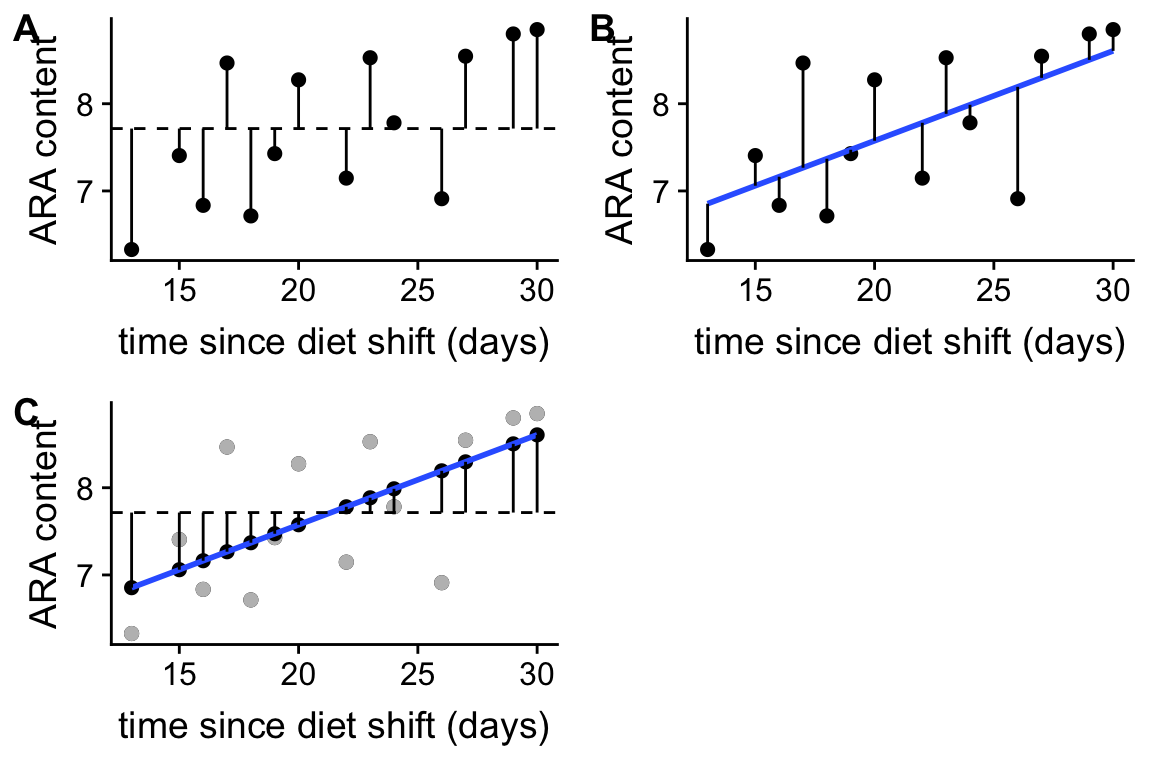
\includegraphics{Walker-elementary-statistical-modeling-draft_files/figure-latex/ols-deviations-1.pdf}
\caption{\label{fig:ols-deviations}Three kinds of deviations from a fit
model. A. Deviations of the measured values from the mean. These are in
the numerator of the equation of the sample variance. The dashed line is
the mean ARA content. B. Deviations of the measured values from the
modeled values. The sum of these deviations squared is what is minimized
in an OLS fit. C. Deviations of the modeled values from the mean ARA
content. The measured values are in gray, the modeled values in black}
\end{figure}

Figure \ref{fig:ols-deviations}A shows the deviations from the measured
values to the mean value (dashed line). These are the deviations in the
numerator of the equation to compute the variance of \(ARA_EGG_MG\).
Figure \ref{fig:ols-deviations}B shows the deviations of the measured
values from the modeled values. The sum of these deviations squared is
what is minimized by the OLS fit. The bigger these deviations are, the
worse the model fit. Figure \ref{fig:ols-deviations}C shows the
deviations of the modeled values to the mean value. The bigger these
deviations are, the better the model fit.

The sums of the squares of these deviations (or ``sums of squares'')
have names:

\begin{equation}
\mathrm{SS(total)} = \sum{(y_i - \bar{y})^2}
\end{equation}

\begin{equation}
\mathrm{SS(error)} = \sum{(y_i - \hat{y_i})^2}
\end{equation}

\begin{equation}
\mathrm{SS(model)} = \sum{(\hat{y_i} - \bar{y})^2}
\end{equation}

Again, \(\mathrm{SS(total)}\) is the numerator of the equation for the
sample variance. It is called ``s-s-total'' because
\(\mathrm{SS(total)} = \mathrm{SS(model)} + \mathrm{SS(error)}\). That
is, the total sums of squares can be \textbf{decomposed} into two
\textbf{components}: the modeled sums of squares and the error sums of
squares. Given these components, it's easy to understand \(R^2\)

\begin{equation}
R^2 = \frac{SS(model)}{SS(total)}
\end{equation}

\(R^2\) is the fraction of the total sums of squares that is due to (or
``explained by'') the model sums of squares. Above I said that \(R^2\)
is the fraction of \emph{variance} explained by the model. Equation xxx
is a ratio of variance, but the \((n-1)^{-1}\) in both the numerator and
the denominator cancel out. Finally, many sources give the equation for
\(R^2\) as

\begin{equation}
R^2 = 1- \frac{SS(error)}{SS(total)}
\end{equation}

which is an obvious alternative given the decomposition. I prefer the
former equation because it emphasizes the model fit instead of model
ill-fit.

\chapter{\texorpdfstring{A linear model with a single, categorical
\emph{X}}{A linear model with a single, categorical X}}\label{a-linear-model-with-a-single-categorical-x}

\section{\texorpdfstring{A linear model with a single, categorical
\emph{X} is the engine behind a single factor (one-way) ANOVA and a
t-test is a special case of this
model.}{A linear model with a single, categorical X is the engine behind a single factor (one-way) ANOVA and a t-test is a special case of this model.}}\label{a-linear-model-with-a-single-categorical-x-is-the-engine-behind-a-single-factor-one-way-anova-and-a-t-test-is-a-special-case-of-this-model.}

To introduce modeling with a single, categorical \(X\) variable, I'll
use the vole data from

\begin{enumerate}
\def\labelenumi{\arabic{enumi}.}
\tightlist
\item
  Source: Dryad Digital Repository.
  \url{https://doi.org/10.5061/dryad.31cc4/1}
\item
  File: ``RSBL-2013-0432 vole data.xlsx''
\item
  Sheet: ``COLD VOLES LIFESPAN''
\end{enumerate}

Normal cellular metabolism creates reactive oxygen species (ROS) that
can disrupt cell function and potentially cause cell damage.
Anti-oxidants are molecules that bind ROS, inhibiting their ability to
disrupt cell activity. A working hypothesis for many years is that
supplemental anti-oxidants should improve cell function and, scaling up,
whole-animal function (such as lifespan). The vole data explores this
with supplemental Vitamins C and E, which are anti-oxidants, in the diet
of the short-tailed field vole (\emph{Microtus agrestis}).

The goal of the study is to measure the effect of anti-oxidants on
lifespan. The researchers randomly assigned the voles to one of thre
treatment levels: ``control'', ``vitamin E'', and ``vitamin C''. The
variable \(treatment\), is a single, categorical \(X\) variable.
Categorical variables are often called \textbf{factors} and the
treatment levels are often called \textbf{factor levels}. There are no
units to a categorical \(X\) variable (even though a certain amount of
each anti-oxidant was supplemented). The response (\(Y\)) is
\(lifespan\) measured in days.

The linear model with a categorical \(X\) variable with three levels is
not immediately obvious, and so I don't present the model until after
showing the table of model coefficients

\subsection{Table of model
coefficients}\label{table-of-model-coefficients}

Here is the table of coefficients from the linear model fit

\begin{tabular}{l|r|r|r|r}
\hline
  & Estimate & Std. Error & t value & Pr(>|t|)\\
\hline
(Intercept) & 503.4 & 27.4 & 18.4 & 0.000\\
\hline
treatmentvitamin\_E & -89.9 & 52.5 & -1.7 & 0.090\\
\hline
treatmentvitamin\_C & -115.1 & 54.5 & -2.1 & 0.037\\
\hline
\end{tabular}

The table has estimates for three parameters. The first estimate (the
intercept) is the mean response in the reference level. Here the
reference level is the ``control'' group. The additional estimates are
the differences in the mean between each of the other treatment levels
and the reference level. These are the ``effects'' in the model. So
typically with categorical \(X\), when we speak of an \emph{effect} we
mean a difference in means. These estimates and their meaning are
illustrated in Figure \ref{fig:vole-mean-plot}.

(note. The default in R is to set the level that is first alphabetically
as the reference level. In the vole data, ``control'' comes before
``vitamin\_E'' and ``vitamin\_C'' alphabetically, and so by default, it
is the reference level. This makes sense for these data -- we want to
compare the lifespan of the vitamins E and C groups to that of the
control group. The reference level can be changed of course.)

\begin{figure}
\centering
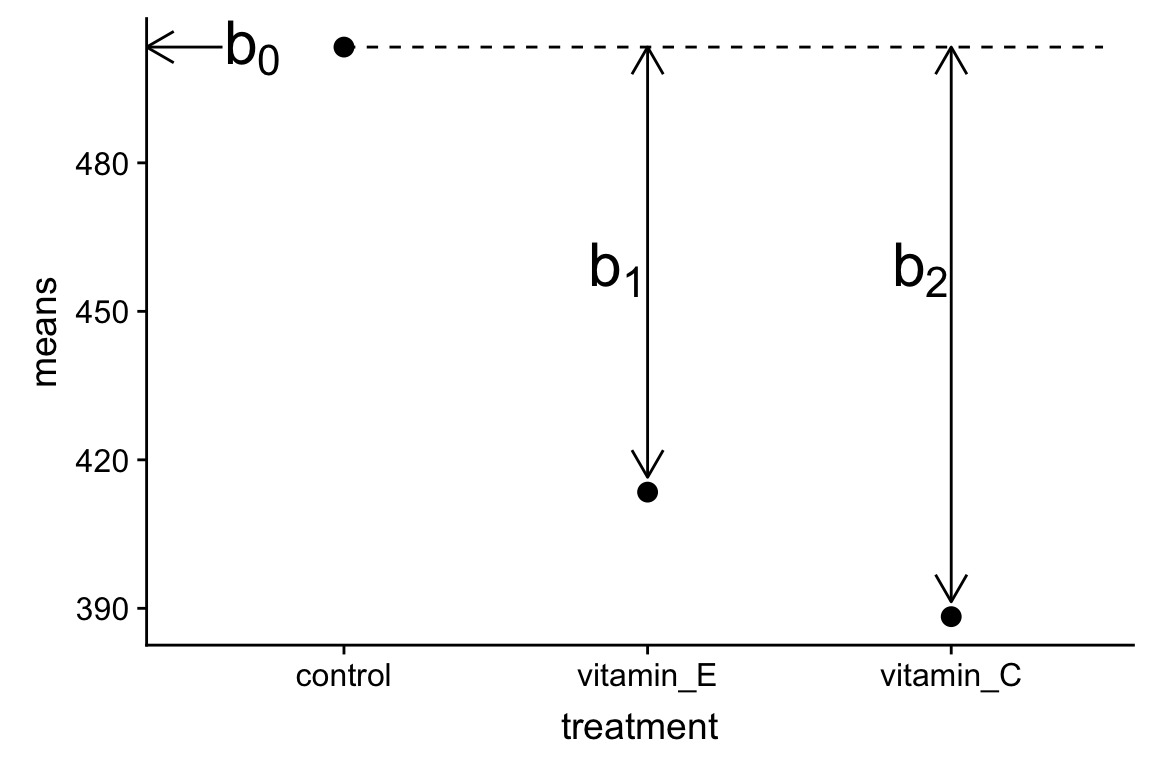
\includegraphics{Walker-elementary-statistical-modeling-draft_files/figure-latex/vole-mean-plot-1.pdf}
\caption{\label{fig:vole-mean-plot}What the coefficients of a linear model
with a single categorical X mean. The means of the three treatment
levels for the vole data are shown with the filled circles. The length
of the double-headed arrows are differences in means. The intercept
(\(b_0\)) is the mean of the reference treatment level. The coefficients
(\(b_1\) and \(b_2\)) are the differences between the treatment level's
mean and the reference mean. As with a linear model with a continuous X,
the coefficients are effects.}
\end{figure}

\subsection{The linear model}\label{the-linear-model}

We can see an immediate difference between the coefficient table for a
linear model fit to a single, categorical \(X\) and that for a single,
continuous \(X\). For the latter, there is a single coefficient for
\(X\). For the former, there is a coefficient for each level of the
categorical \(X\) \emph{except} the ``reference'' level.

The linear model for a single, continuous \(X\) with three factor levels
is

\begin{equation}
lifespan = \beta_0 + \beta_1 vitamin\_E + \beta_2 vitamin\_C + \varepsilon
\end{equation}

and the estimates in the coefficient table are the coefficients of the
fit model

\begin{equation}
lifespan_i = b_0 + b_1 vitamin\_E + b_2 vitamin\_C + e_i
\label{eq:model-cat-x}
\end{equation}

Remember, \(b_0\) is the mean of the control group, \(b_1\) is the
difference in means between the vitamin E and control groups, and
\(b_2\) is the difference in means between the vitamin C and control
groups (Figure \ref{fig:vole-mean-plot}).

In this model, \(vitamin\_E\) and \(vitamin\_C\) are \textbf{dummy
variables} that contain a one, if the data is from that treatment level,
and zero otherwise. This is called dummy coding or treatment coding. The
\texttt{lm} function creates these dummy variables under the table, in
something called the \textbf{model matrix}, which we'll cover in the
next chapter. You won't see these columns in your data. But if you did,
it would look something like this

\begin{tabular}{r|l|r|r}
\hline
lifespan & treatment & vitamin\_E & vitamin\_C\\
\hline
621 & control & 0 & 0\\
\hline
865 & control & 0 & 0\\
\hline
583 & vitamin\_E & 1 & 0\\
\hline
561 & vitamin\_E & 1 & 0\\
\hline
315 & vitamin\_C & 0 & 1\\
\hline
157 & vitamin\_C & 0 & 1\\
\hline
\end{tabular}

There are alternative coding methods. Dummy coding is the default in R.
Note that the method of coding can make a difference in an ANOVA table,
and many published papers using R have published incorrect
interpretations of ANOVA table outputs. This is both getting ahead of
ourselves and somewhat moot, because I don't advocate publishing ANOVA
tables.

\subsubsection{\texorpdfstring{Some math to convince you that the
intercept of a linear model with a categorical \(X\) is the mean of the
reference group \emph{and} the intercept of a line. And some math to
convince you that the coefficient of a dummy variable in a linear model
with a categorial \(X\) is a difference in means \emph{and} a
slope.}{Some math to convince you that the intercept of a linear model with a categorical X is the mean of the reference group and the intercept of a line. And some math to convince you that the coefficient of a dummy variable in a linear model with a categorial X is a difference in means and a slope.}}\label{some-math-to-convince-you-that-the-intercept-of-a-linear-model-with-a-categorical-x-is-the-mean-of-the-reference-group-and-the-intercept-of-a-line.-and-some-math-to-convince-you-that-the-coefficient-of-a-dummy-variable-in-a-linear-model-with-a-categorial-x-is-a-difference-in-means-and-a-slope.}

The interecept of a model is the value of the model when all
\(X\)-variables are set to zero. The \(X\) variables in the model
(Equation \eqref{eq:model-cat-x}) are the dummy variables \(vitamin\_E\)
and \(vitamin\_C\). If we set vitamin\_E\$ and \(vitamin\_C\) in
Equation \eqref{eq:model-cat-x} to zero, the modeled (or expected) value
reduces to

\begin{equation}
\mathrm{E}(lifespan|X_1=0, X_2=0) = b_0
\end{equation}

\% Since both dummy variables are set to zero, we have modeled the
expected value or mean of the control group.

The slope of a model is the difference in the modeled value given a one
unit increase in \(X\). If we increase the dummy variable \(vitamin\_E\)
from zero to one (that is, if we are modeling the expected value of the
vitamin E group), we get

\begin{equation}
\mathrm{E}(lifespan|X_1=1, X_2=0) = b_0 + b_1
\end{equation}

which can be re-arranged to

\begin{equation}
b_1 = \mathrm{E}(lifespan|X_1=1, X_2=0) - b_0
\end{equation}

and since \(\mathrm{E}(lifespan|X_1=0, X_2=0) = b_0\) then

\begin{equation}
b_1 = \mathrm{E}(lifespan|X_1=1, X_2=0) - \mathrm{E}(lifespan|X_1=0, X_2=0)
\end{equation}

or, the coefficient of vitamin E is the difference in means between the
vitamin E and control groups, which is also a slope since this is the
expected difference given a one unit increase in \(vitamin\_E\).

\subsection{Reporting results}\label{reporting-results-1}

What should be reported for the analyis of effects of anti-oxidant
supplements on vole lifespan? Best practice includes reporting the raw
data with a summary distribution and treatment effects with CIs. ``Raw
data'' means the individual lifespans as a function of treatment level.

\subsubsection{Harrel Plot of the data}\label{harrel-plot-of-the-data}

\begin{figure}
\centering
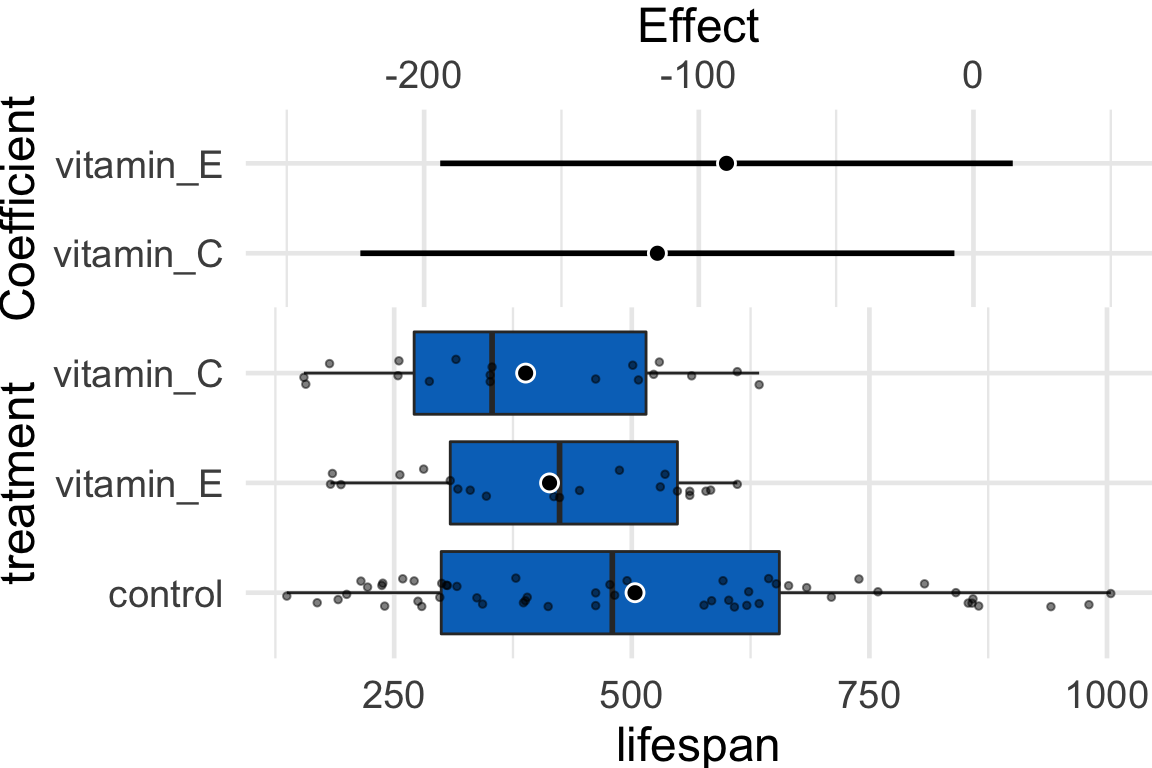
\includegraphics{Walker-elementary-statistical-modeling-draft_files/figure-latex/harrellplot-1.pdf}
\caption{\label{fig:harrellplot}HarrellPlot of the raw data, distribution,
and effects of the vole lifespan data.}
\end{figure}

The raw data, the distributions within treatment level, and the effects
(difference in means) of treatment can be combined into a single plot
that I call a Harrell plot (Figure \ref{fig:voles}). Notice that the
\emph{x}-axis and \emph{y} axes are flipped so that \(lifespan\) is on
the \emph{x}-axis. It is still the ``response'' or ``Y'' variable! The
Harrell plot contains two parts

\begin{enumerate}
\def\labelenumi{\arabic{enumi}.}
\tightlist
\item
  The bottom contains a \textbf{strip chart} (often called a ``dot
  plot'') of the raw response measures grouped by factor level.
  Superimposed over the strip chart is a \textbf{box plot} summarizing
  the distribution of each factor level. The line in the center of a box
  is the median \(lifespan\) for that group, the left and right edges of
  the box are the 25\% and 75\% quantiles of \(lifespan\) for that grop,
  and the lines extending to the left and right of the box are the
  ``whiskers'', which are the smallest and largest value within
  \(1.5 IQR\) (inter-quartile range, which is the interval bounded by
  box).
\item
  The top is a \textbf{forest plot} of the effects and the 95\% CI of
  the effects. For categorical \(X\), the effects could be model
  coefficients or treatment \textbf{contrasts}, which are differences in
  means between treatment levels. Model coefficients are a subset of
  possible treatment contrasts.
\end{enumerate}

The Harrell plot above shows the effects as model coefficients, which
(again!) are differences between the mean of the response in a specific
treatment level and the mean of the response in a reference level. Here
the reference level is the control group.

\subsubsection{In-text reporting}\label{in-text-reporting}

``The mean lifespan of cold-reared voles supplmented with vitamin E was
-89.9 days shorter than the mean lifespan for the control group (95\%
CI: -194.1, 14.3). The mean lifespan of cold-reared voles supplmented
with vitamin C was -115.1 days shorter than the mean lifespan for the
control group (95\% CI: -223.2, -6.9).

\subsubsection{Correct interpretation of the Confidence Interval is
key}\label{correct-interpretation-of-the-confidence-interval-is-key}

Remember, that the CI contains the range of parameter values that are
consistent with the data (in the sense that a t-test wouldn't reject the
hypothesis test). This means that a true value at the low end or the
high end of the CI is consistent with the data. Your technical
report/manuscript should discuss the consequences of this. For example,
A small, increase in lifespan is consistant with the Vitamin E but not
Vitamin C supplementation, if we use the 95\% CI as a pretty good range
for inferring ``consistent with''. Both a 223 day and a 7 day decrease
in lifespan are consistant with the Vitamin C effect. 223 days seems
like a huge effect, especially for a short lived vole. 7 days is
certainly a much smaller effect, but this doesn't mean that it doesn't
have important ecological, behavioral, or fitness consequences.

\section{Working in R}\label{working-in-r-1}

\subsection{\texorpdfstring{Exploring the relationship between \emph{Y}
and
\emph{X}}{Exploring the relationship between Y and X}}\label{exploring-the-relationship-between-y-and-x}

Questions

\begin{enumerate}
\def\labelenumi{\arabic{enumi}.}
\tightlist
\item
  Import the vole data from the Dryad repository as the data.table
  \texttt{vole\_wide}. Replace the spaces in the column labels with the
  underscore ``\_``.
\end{enumerate}

The data are in ``wide'' format. A pretty good script for for converting
these to long format is

\begin{Shaded}
\begin{Highlighting}[]
\NormalTok{vole_long <-}\StringTok{ }\KeywordTok{melt}\NormalTok{(vole_wide, }\DataTypeTok{measure.vars=}\KeywordTok{c}\NormalTok{(}\StringTok{"control"}\NormalTok{, }\StringTok{"vitamin_E"}\NormalTok{, }\StringTok{"vitamin_C"}\NormalTok{), }\DataTypeTok{variable.name=}\StringTok{"treatment"}\NormalTok{)}
\NormalTok{vole <-}\StringTok{ }\KeywordTok{na.omit}\NormalTok{(vole_long)}
\CommentTok{# melt is from reshape2 package and is a workhorse in R}
\CommentTok{# the resulting data frame has 3 stacked copies of the same rows}
\CommentTok{# na.omit removes the superfluous two extra sets of rows created by melt}
\CommentTok{# the more compact way to do this is combine the steps:}
\CommentTok{# vole <- na.omit(melt(vole_wide, measure.vars=c("control", "vitamin_E", "vitamin_C"))}
\CommentTok{# but I suggest two steps so you can see what melt does. This isn't the best example of using melt.}
\end{Highlighting}
\end{Shaded}

Use the ggpubr package to create a box plot, grouped by treatment, with
superimposed strip chart (``dots'')

Questions

\begin{enumerate}
\def\labelenumi{\arabic{enumi}.}
\setcounter{enumi}{1}
\tightlist
\item
  Do the response as a function of group look fairly normally
  distributed or are there red flags such as skewness, outliers, bimodal
  clusters, etc.
\item
  Is the direction of the effect consistent with the expected direction?
\end{enumerate}

\subsection{Fitting the model}\label{fitting-the-model}

As with a single, continuous \(X\), we fit the model using the
\texttt{lm} function and with the model formula of the form
\texttt{y\ \textasciitilde{}\ x}. Note that the R formula can use the
single categorical variable \(treatment\). The code underneath lm will
note that \(treatment\) is a factor with three levels and will
automatically create the two dummy variables noted above in the linear
model.

\begin{Shaded}
\begin{Highlighting}[]
\NormalTok{fit <-}\StringTok{ }\KeywordTok{lm}\NormalTok{(lifespan }\OperatorTok{~}\StringTok{ }\NormalTok{treatment, }\DataTypeTok{data=}\NormalTok{vole)}
\end{Highlighting}
\end{Shaded}

All of the same scripts to access the information in \texttt{fit} that
we used with the continuous \(X\) analysis are the same. For example,
the base R \texttt{summary} function gives the same information as in
the continuous \(X\) example.

Questions

\begin{enumerate}
\def\labelenumi{\arabic{enumi}.}
\setcounter{enumi}{3}
\tightlist
\item
  Review different output in the \texttt{summary} function and list
  which are useful and which are not so useful and why.
\end{enumerate}

Other useful functions on the lm object (``fit'') are
\texttt{coefficients(summary())}, \texttt{coef()} or
\texttt{coefficients()} and \texttt{confint}. Assigning the output of
these functions to an R object allows you to increase reproducibility.
For example, if I assign the coefficients to \texttt{b}

\begin{Shaded}
\begin{Highlighting}[]
\NormalTok{b <-}\StringTok{ }\KeywordTok{coef}\NormalTok{(fit)}
\end{Highlighting}
\end{Shaded}

then I can report these in R markdown text by embedding r code directly
in the text. For example, if I embed ``r
round(b{[}``treatmentvitamin\_E''{]}, 1)'' between a pair of single
accent characters, then r markdown inserts -89.9 into the rendered text.

\subsection{An introduction to
contrasts}\label{an-introduction-to-contrasts}

We often want to compare more than just the non-reference levels to the
reference level. For example, we might want to compare the effects of
the vitamin E supplementation to vitamin C supplementation. Or, we might
want to combine (or ``pool'') vitamin C and vitamin E levels effects
into a single ``anti-oxidant'' level and compare to the control. These
comparisons of means are called linear \textbf{contrasts}. The emmeans
package is a good package for obtaining contrasts for both simple linear
models computed with \texttt{lm} and for more complicated statistical
models. If you haven't already, download the emmeans package.

\begin{Shaded}
\begin{Highlighting}[]
\NormalTok{fit.em <-}\StringTok{ }\KeywordTok{emmeans}\NormalTok{(fit, }\DataTypeTok{spec=}\StringTok{"treatment"}\NormalTok{)}
\NormalTok{fit.em}
\end{Highlighting}
\end{Shaded}

\begin{verbatim}
##  treatment   emmean       SE df lower.CL upper.CL
##  control   503.3929 27.40978 93 448.9625 557.8233
##  vitamin_E 413.4762 44.75999 93 324.5917 502.3607
##  vitamin_C 388.3158 47.05685 93 294.8702 481.7614
## 
## Confidence level used: 0.95
\end{verbatim}

The \texttt{emmeans()} function returns various estimated means,
depending on what is specified with the \texttt{spec=} parameter. Here
the grouping variable ``treatment'' is specified, so the means returned
are estimates of \(\mathrm{E}(lifespan | treatment)\), the modeled means
for each level of treatment. For this simple analysis, the modeled means
are simply the group means. Note that the default value returned is a
table with the standard error and 95\% confidence limits of the
estimates.

Let's use the emmeans object to get the contrasts for all combinations
of treatment levels.

\begin{Shaded}
\begin{Highlighting}[]
\KeywordTok{summary}\NormalTok{(}\KeywordTok{contrast}\NormalTok{(fit.em, }\DataTypeTok{method=}\StringTok{"revpairwise"}\NormalTok{, }\DataTypeTok{adjust=}\StringTok{"none"}\NormalTok{), }\DataTypeTok{infer=}\KeywordTok{c}\NormalTok{(}\OtherTok{TRUE}\NormalTok{, }\OtherTok{TRUE}\NormalTok{))}
\end{Highlighting}
\end{Shaded}

\begin{verbatim}
##  contrast                estimate       SE df  lower.CL   upper.CL t.ratio
##  vitamin_E - control    -89.91667 52.48574 93 -194.1429  14.309609  -1.713
##  vitamin_C - control   -115.07707 54.45772 93 -223.2193  -6.934834  -2.113
##  vitamin_C - vitamin_E  -25.16040 64.94462 93 -154.1275 103.806738  -0.387
##  p.value
##   0.0900
##   0.0373
##   0.6993
## 
## Confidence level used: 0.95
\end{verbatim}

I've sent to parameters to the contrast function and one to the summary
function

\begin{enumerate}
\def\labelenumi{\arabic{enumi}.}
\tightlist
\item
  method=``revpairwise''. \texttt{contrast} can create different
  combinations of differences between means. Here I've specified all
  pairwise differences (the ``rev'' reverses the order of the
  subtraction). Notice that the statistics (estimate, SE, etc) are equal
  to the same statistics for \(b_1\) and \(b_2\) of the linear model. I
  said earlier that these coefficients are contrasts!
\item
  adjust=``none''. In classical frequentist hypothesis testing, the
  p-value of a contrast in what are called ``post-hoc tests'' is
  adjusted to reflect ``multiple testing'' (more than one p-value is
  being computed). This adjustment is almost standard in biology, but
  the practice is hugely controversial. The concept of multiple testing
  is important, and we will return to this in a future chapter, but here
  I have chosen to show the unadjusted p-value. The reason is that I
  want the unadjusted confidence interval and the adjustment would
  adjust these as well. If deleted \texttt{adjust="none"} from the
  script, the contrast function would default to the \textbf{Tukey HSD}
  (Honestly Significant Difference) test. There are literally dozens and
  dozens of post-hoc tests, which largely reflects the misplaced
  emphasis on ``better'' \(p\)-values rather than parameter estimates
  and their uncertainty.
\item
  infer=c(TRUE, TRUE). This parameter controls what kind of inference to
  put in the table. The first value specifies the inclusion of the CI
  (emmeans uses ``CL'' for confidence limit), the second value specifies
  the inclusion of \(t\) and \(p\)-values.
\end{enumerate}

\subsection{Harrell plot}\label{harrell-plot}

\subsubsection{Installing the harrellplot
package}\label{installing-the-harrellplot-package}

The harrellplot package is available on github but not a cran repository
and, therefore, takes a little more work to install. To install a
package from a github repository, 1. load library(devtools) -- this may
need to be installed first using the R Studio Tools \textgreater{}
Install Packages\ldots{} tool 2. install harrellplot from github. In the
console, type

\texttt{install\_github("middleprofessor/harrellplot")}

\begin{enumerate}
\def\labelenumi{\arabic{enumi}.}
\setcounter{enumi}{2}
\tightlist
\item
  load the harrellplot package
\item
  harrellplot requires other packages including broom, Hmisc, car, lme4,
  and lmerTest. If you haven't installed these do. load these with the
  library() function at the start of your notebook.
\end{enumerate}

\subsubsection{Using harrellplot to make a nice, publishable plot of
treatment
effects}\label{using-harrellplot-to-make-a-nice-publishable-plot-of-treatment-effects}

In the console type `?harrellplot to see the many parameters. Unlike
ggplot2, variable names need to be specified with quotes in the
harrellplot function. The harrellplot function is a list with several
elements.

Here is the default plot

\begin{Shaded}
\begin{Highlighting}[]
\NormalTok{vole.harrellplot <-}\StringTok{ }\KeywordTok{harrellplot}\NormalTok{(}\DataTypeTok{x=}\StringTok{"treatment"}\NormalTok{, }\DataTypeTok{y=}\StringTok{"lifespan"}\NormalTok{, }\DataTypeTok{data=}\NormalTok{vole)}
\NormalTok{vole.harrellplot}\OperatorTok{$}\NormalTok{gg }\CommentTok{# gg is the plot object}
\end{Highlighting}
\end{Shaded}

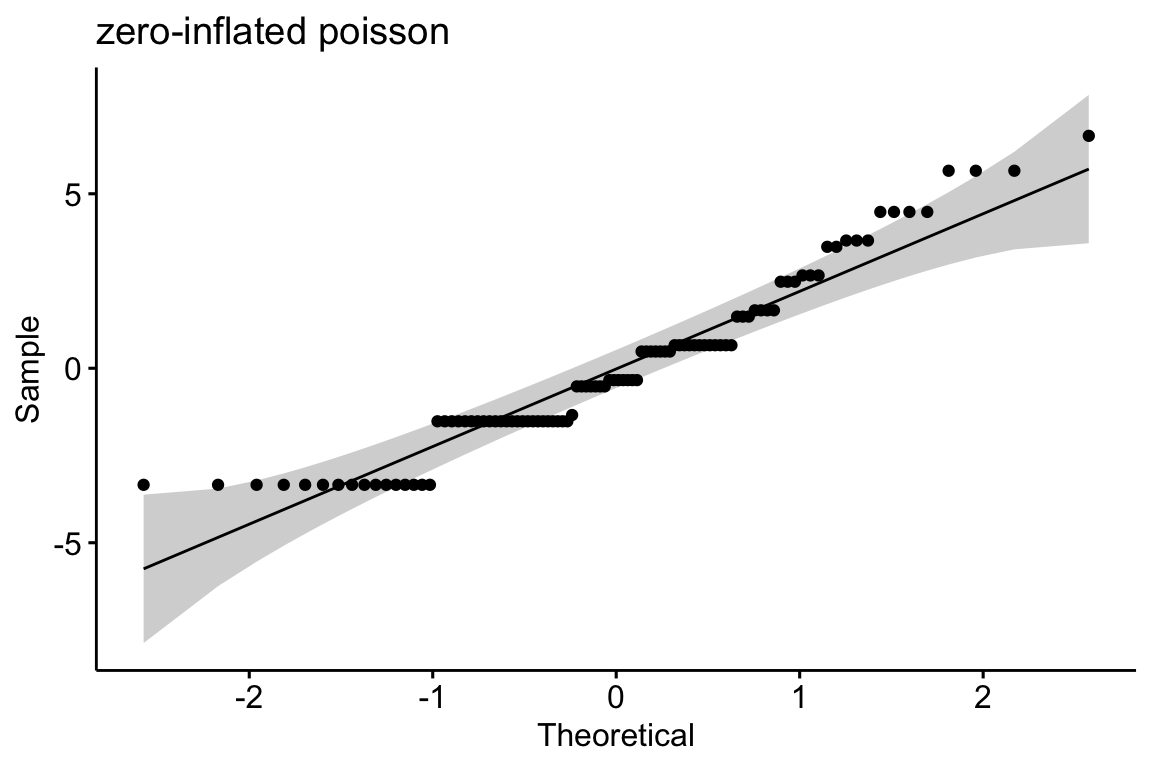
\includegraphics{Walker-elementary-statistical-modeling-draft_files/figure-latex/unnamed-chunk-12-1.pdf}

\chapter{P-values}\label{p-values}

\section{\texorpdfstring{\(p\)-values}{p-values}}\label{p-values-1}

\begin{tabular}{l|r|r|r|r|r|r|r}
\hline
contrast & estimate & SE & df & lower.CL & upper.CL & t.ratio & p.value\\
\hline
vitamin\_E - control & -89.9 & 52 & 93 & -194.1 & 14.3 & -1.7 & 0.090\\
\hline
vitamin\_C - control & -115.1 & 54 & 93 & -223.2 & -6.9 & -2.1 & 0.037\\
\hline
vitamin\_C - vitamin\_E & -25.2 & 65 & 93 & -154.1 & 103.8 & -0.4 & 0.699\\
\hline
\end{tabular}

Let's use the vole data to introduce the \(p\)-value. The table above
gives a SE, \(t\) and \(p\)-value for each pairwise contrast among the
three treatment levels. A typical report (one with several
misconceptions) might read

``We found a significant effect of Vitamin C (\(t=\) -2.1, \(p=\) 0.037)
on lifespan, but no effect of vitamin E (\(t=\) -1.7, \(p=\) 0.09) on
lifespan.''

A \(p\) value \emph{is a continuous measure of evidence against the
null}. As long as the data approximate the assumptions of the null
hypothesis pretty well, a very small \(p\)-value, such as 0.002 or
0.0005, is pretty good evidence against the null hypothesis -- but does
not mean ``an effect exists''. To show an effect exists, we should have
small \(p\)-values in multiple replicates \emph{and} we should
rigorously probe the hypothesis with different experiments that
challenge the hypothesis in different ways. A small \(p\) is evidence
for a research program to move forward with replication and probing. A
big \(p\)-value, say 0.22 or 0.76, is pretty weak evidence against the
null, but does not mean ``there is no effect.'' If an experiment is well
designed, a big \(p\) could suggest abandoning any hypotheses that
predict biologically consequential effects. Unfortunately, a big \(p\)
could also reflect a weak experimental design. Between small and big
\(p\) values, such as 0.009 or 0.011, problems arise. These intermediate
\(p\)-values beg for replication. A major problem of inference using
\(p\) values is that there is no sharp boundaries between these three
regions. Instead biologists typically use the \(p < 0.05\) as a sharp
boundary to declare that an effect exists or not.

Okay. so what \emph{is} a \(p\)-value? When we do a \(t\)-test, we get a
\(p\)-value. There are several ways to think about this probability. The
most compact way is \(P(data | null)\), which is literally read as the
probability of the data given the null (or ``conditional'' on the null),
but is really short for \emph{the probability of the data, or something
more extreme than the data, given that the null hypothesis is true}. The
``probability of the data'' is kinda vague. More specifically, we mean
the probability of some statistic about the data such as the difference
in means between group A and group B or the \(t\)-value associated with
this difference. So, a bit more formally, the probability returned in a
\(t\)-test is \(\mathrm{prob}(t \ge t_{obs} | H_0)\). This is the long
run frequency of observing a \(t\)-value as big or bigger than the
observed \(t\)-value (the one you actually got with your data) if the
null is true. Let's parse this into ``long run frequency of observing a
\(t\)-value as big or bigger than the observed \(t\)-value'' and ``null
is true''.

A thought experiment: You open a google sheet and insert 12 standard,
normal random deviates (so the true mean is zero and the true variance
is one) in Column A, rows 1-12. You arbitrarily assign the first six
values (rows 1-6) to treatment A and the second six values (rows 7-12)
to treatment B. You use the space immediately below these data to
compute the mean of treatment A, the mean of treatment B, the difference
in means (A - B), and a \(t\)-value. Unfortunately, google sheets
doesn't have a \(t\)-value function so you'd have to compute this
yourself. Or not, since this is a thought experiment. Now ``fill right''
or copy and paste these functions into 999 new columns. You now have
1000 \(t\) tests. The expected value of the difference in means is zero
(why?) but the actual values will form a normal distribution about zero.
Most will be close to zero (either in the negative or positive
direction) but some will be further from zero. The expected \(t\)-value
will also be zero (why?) and the distribution of these 1000 \(t\) values
will look normal but the tails are a little fuller. This row of \(t\)
values is a null distribution, because in generating the data we used
the exact same formula for the values assigned to A and the values
assigned to B. Now think of a \(t\)-value in your head, say 0.72
(remember that \(t\) values will largely range from about -3 to +3
although the theoretical range is \(-\infty\) to \(+\infty\). What is
the probability of observing a \(t\) of 0.72 \emph{or bigger} if the
null is true? Look at the row of \(t\)-values! Count the number of
\(t \ge 0.72\) and then divide by the total number of \(t\)-values in
the row (1000) and you have a probability computed as a frequency. But
remember the frequentist definition is the long run frequency, or the
expected frequency at the limit (when you've generated not 1000 or even
1,000,000 but an infinite number of columns and \(t\)-values).

Some asides to the thought experiment: First, why ``as big or bigger''
and not just the probability of the value itself? The reason is that the
probability of finding the exact \(t\) is 1/infinity, which doesn't do
us much good. So instead we compute the probability of finding \(t\) as
big, or bigger, than our observed \(t\). Second, the \(t\)-test
probability described above is a ``one-tail probability''. Because a
difference can be both in the positive direction and the negative
direction, we usually want to count all the \(t \ge 0.72\) and the
\(t \le -0.72\) and then add these two counts to compute the frequency
of \emph{as extreme or more extreme} values. This is called a
``two-tailed probability'' because we find extremes at both tails of the
distribution. Third, we don't really count \(t \ge 0.72\) but take
advantage of the beautiful mathematical properties of the theoretical
\(t\) distribution, which allows us to compute the frequentist
probability (expected long range frequency) given the \(t\)-value and
the degrees of freedom using the \(t\)-distribution.

Now what do I mean with the phrase ``null is true''? Most people equate
``null is true'' with ``no difference in means'' but the phrase entails
much more than this. Effectively, the phrase means that the \(p\)-value
is based on modeling the real data with a theoretical sample in which
all the points were randomly sampled from the same distribution and that
the assignment of the individual points to treatment was random. This
model means the theoretical sample has three properties: First, random
assignment to treatment after sampling from the same distribution means
that the expected means are the same, or put differently, the expected
difference in means between the assigned groups is zero. Second, random
assignment to treatment after sampling from the same distribution
\emph{also} means that the expected variances of the two groups are
equal. And third, random sampling means that the values of each point
are independent -- we cannot predict the value of one point knowing
information about any other point. \textbf{Here is what is super
important about this}: if we get a really low \(p\)-value, any one of
these consequences may be untrue about our data, for example it could be
that the true means of the two treatment groups really are different, or
it could mean it is the variances that differ between the two groups, or
it could mean that the data (or technically, the errors) are not
independent of each other. This is why we need certain assumptions to
make a \(p\)-value meaningful for empirical data. By assuming
independent error and homogenous (equal) variances in our two samples, a
low \(p\) value is evidence of unequal means.

\section{Creating a null
distribution.}\label{creating-a-null-distribution.}

Let's repeat: A pretty good definition of a \(p\)-value is: the long-run
frequency of observing a test-statistic as large or larger than the
observed statistic, if the null were true. A more succinct way to state
this is

\begin{equation}
p = \mathrm{prob}(t \ge t_o | H_o)
\end{equation}

where \(t\) is a hypothetically sampled \(t\)-value from a null
distribution, \(t_o\) is the observed \(t\)-value, and \(H_o\) is the
null hypothesis. Part of the null hypothesis is the expected value of
the parameter estimated is usually (but not always) zero -- this can be
called the nil null. For example, if there is no vitamin E effect on
lifespan, then the expected difference between the means of the control
and vitamin E treatment levels is zero. Or,

\begin{equation}
\mathrm{E}(\bar{vitamin_E} - \bar{control} | H_o) = 0.0
\end{equation}

let's plot the data and look at the group means. Below is a strip chart
of the vole data with superimposed treatment level means, using the
function \texttt{ggstripchart} from the ggpubr package (can you make
this?). I'm going to refer to this kind of chart as a ``dot plot'',
which is what most biology researchers call this type of chart.

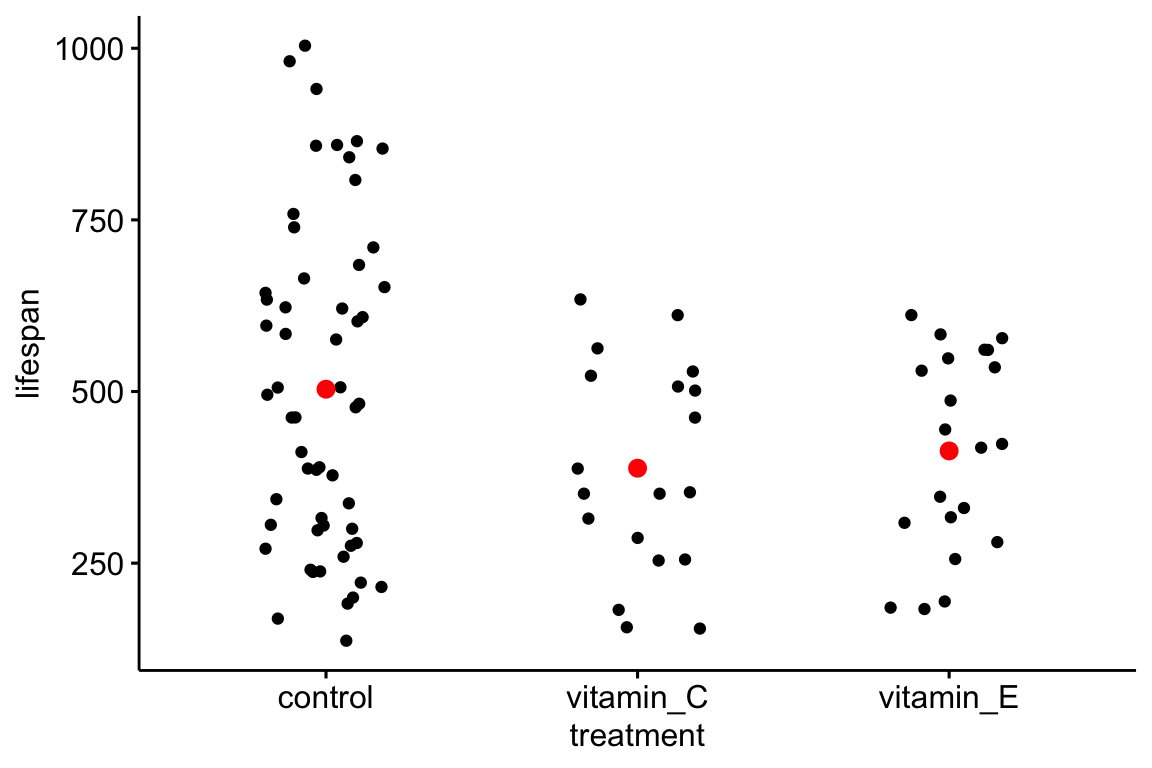
\includegraphics{Walker-elementary-statistical-modeling-draft_files/figure-latex/inference-strip-chart-1.pdf}

\subsection{the Null Distribution}\label{the-null-distribution}

The mean lifespan in the vitamin\_E treatment is -89.9 days shorter than
the mean lifespan in the control treatment. And, the mean lifespan in
the vitamin\_E treatment is -115.1 days shorter than the mean lifespan
in the control treatment. These are the measured effects, or the
\textbf{observed differences in means}. How confident are we in these
effects? Certainly, if the researchers did the experiment with
\emph{two} control treatment groups, they would measure some difference
in their means simply because of finite sampling (more specifically, the
many, many random effects that contribute to lifespan will differ
between the two control groups). So let's reframe the question: are the
observed differences unusually large compared to a distribution of
differences that would occur if there were no effect? That is, if the
``null were true''. To answer this, we compare our observed difference
to this \textbf{null distribution}. This comparison gives the
probability (a long-run frequency) of ``sampling'' a random difference
from the null distribution of differences that is as large, or larger,
than the observed difference.

What is a null distribution? It is the distribution of a statistic (such
as a difference in means, or better, a \(t\)-value) if the null were
true. Here, I am generating a null distribution that is relevant to the
cold vole data. See if you can understand the script before reading the
explanation below.

\begin{Shaded}
\begin{Highlighting}[]
\NormalTok{seed <-}\StringTok{ }\DecValTok{1}
\NormalTok{n_iter <-}\StringTok{ }\DecValTok{10}\OperatorTok{^}\DecValTok{5} \CommentTok{# number of iterations}
\NormalTok{mu <-}\StringTok{ }\KeywordTok{mean}\NormalTok{(vole[treatment}\OperatorTok{==}\StringTok{'control'}\NormalTok{, lifespan]) }
\NormalTok{sigma <-}\StringTok{ }\KeywordTok{sd}\NormalTok{(vole[treatment}\OperatorTok{==}\StringTok{'control'}\NormalTok{, lifespan])}
\NormalTok{n <-}\StringTok{ }\KeywordTok{nrow}\NormalTok{((vole[treatment}\OperatorTok{==}\StringTok{'control'}\NormalTok{,]))}
\NormalTok{sample1 <-}\StringTok{ }\KeywordTok{matrix}\NormalTok{(}\KeywordTok{rnorm}\NormalTok{(n}\OperatorTok{*}\NormalTok{n_iter, }\DataTypeTok{mean=}\NormalTok{mu, }\DataTypeTok{sd=}\NormalTok{sigma), }\DataTypeTok{nrow=}\NormalTok{n) }\CommentTok{# 100,000 samples (each size n)}
\NormalTok{sample2 <-}\StringTok{ }\KeywordTok{matrix}\NormalTok{(}\KeywordTok{rnorm}\NormalTok{(n}\OperatorTok{*}\NormalTok{n_iter, }\DataTypeTok{mean=}\NormalTok{mu, }\DataTypeTok{sd=}\NormalTok{sigma), }\DataTypeTok{nrow=}\NormalTok{n) }\CommentTok{# 100,000 samples}
\NormalTok{null_dis <-}\StringTok{ }\KeywordTok{apply}\NormalTok{(sample2, }\DecValTok{2}\NormalTok{, mean) }\OperatorTok{-}\StringTok{ }\KeywordTok{apply}\NormalTok{(sample1, }\DecValTok{2}\NormalTok{, mean)}
\KeywordTok{qplot}\NormalTok{(null_dis)}
\end{Highlighting}
\end{Shaded}

\begin{figure}
\centering
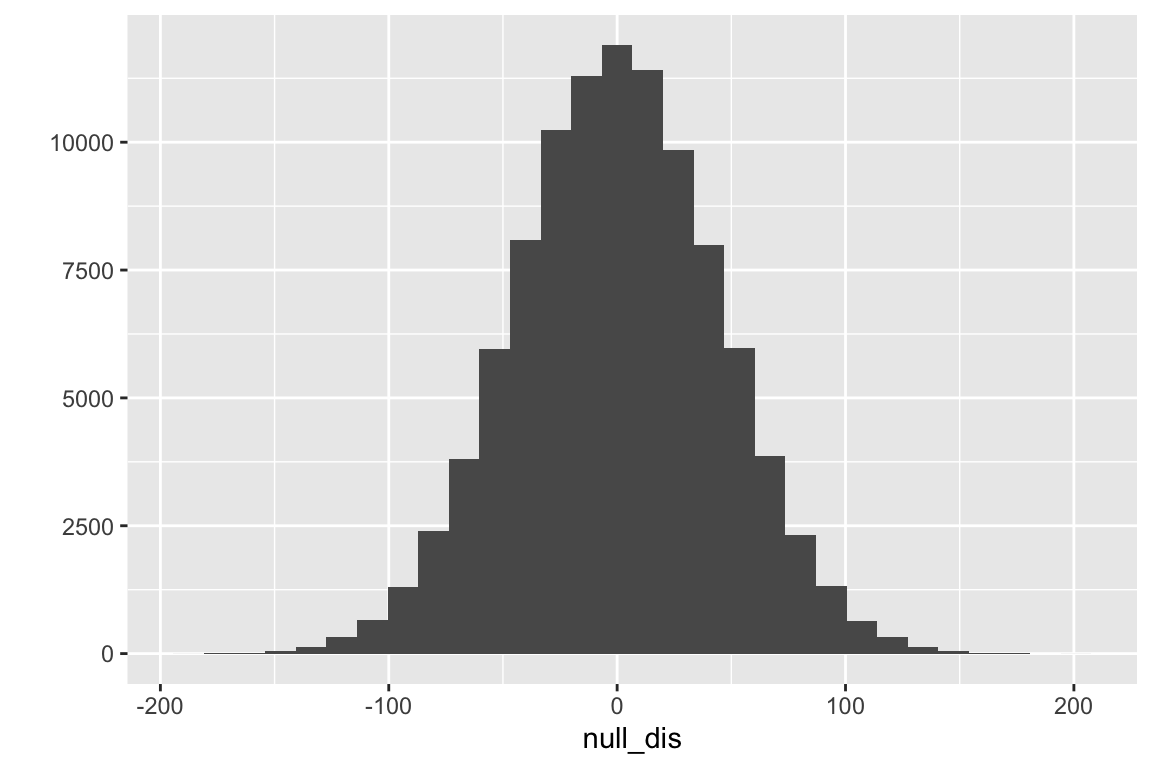
\includegraphics{Walker-elementary-statistical-modeling-draft_files/figure-latex/null-distribution-1.pdf}
\caption{\label{fig:null-distribution}Null distribution for an infinitely
large data set that looks curiously like the lifespans of the cold-rear
voles from the control treatment.}
\end{figure}

What have we done above? We've simulated an infinitely large population
of voles that have a distribution of lifespans similar to that of the
cold-reared voles assigned to the control group. The mean \(\mu\) and
standard deviation \(\sigma\) of the simulated lifespan are equal to the
observed mean and standard deviation of the lifespans of the control
voles. Then, the script:

\begin{enumerate}
\def\labelenumi{\arabic{enumi}.}
\tightlist
\item
  randomly sample 56 values from this population of simulated lifespans
  and assign to sample1. We sample 56 values because that is the sample
  size of our control in the experiment.
\item
  randomly sample 56 values from this population of simulated lifespans
  and assign to sample2.
\item
  compute the difference \(\bar{Y}_{sample2} - \bar{Y}_{sample1}\).
\item
  repeat 1-3 100,000 times, each time saving the difference in means.
\item
  plot the distribution of the 100,000 differences using a histogram
\end{enumerate}

The distribution of the differences is a null distribution. Notice that
the mode of the null distribution is at zero, and the mean (-0.11584) is
close to zero (if we had set \(n\) to infinity, the mean would be
precisely zero). \emph{The expected difference between the means of two
random samples from the same population is, of course, zero}. Don't
gloss over this statement if that is not obvious. The tails extend out
to a little more than +100 and -100. What this means is that it would be
rare to randomly sample two sets of data from the same population with
mean \(\mu\) and standard deviation \(\sigma\) and find a difference of,
say, -257. In fact, in the 100,000 runs, there were no difference as
large as \textbar{}-257\textbar{} (the absolute value of -257). The
minimum and maximum differences sampled over the 100,000 iterations was
-187 days and 201 days.

How do our observed differences compare? Let's focus on vitamin E. The
vitamin\_E effect is -89.9 days. There are 2110 sampled differences less
than the observed value and 2126 greater than the absolute value of the
observed value. Together this is 4236 so the frequency of differences
from the simulated null distribution that as larger or larger than the
observed difference is 0.042 (this compuation includes the observed
value in both the numerator and denominator).

\subsection{\texorpdfstring{\(t\)-tests}{t-tests}}\label{t-tests}

A \(t\)-test is a test of differences between two values. These could be

\begin{enumerate}
\def\labelenumi{\arabic{enumi}.}
\tightlist
\item
  the difference between the means of two samples (a ``two-sample''
  \(t\)-test)
\item
  the difference between a mean of a sample and some pre-specified value
  (a ``one-sample'' \(t\)-test)
\item
  the difference between a coefficient from a linear model and a value
  (often zero)
\end{enumerate}

A \(t\)-test compares an observed \(t\)-value to a \(t\)-distribution.
The null distribution introduced above was a distribution of mean
differences. This isn't generally useful, since the distribution of
expected mean differences is a function of sample variability (standard
deviations) in addition to sample size and, therefore, a mean-difference
null distribution will be unique to every study. A \(t\)-distribution is
a distribution of \(t\)-values under the null (statistical jargon for
``given the null is true''), where a \(t\)-value is a difference
standardized by its standard error. Standardizing by a standard
deviation (remember that a standard error is an estimate of the
statistic's standard deviation) removes the effect of sample variability
on the distribution. A \(t\)-distribution, then, is only a function of
sample size (or ``degrees of freedom''). As \(n\) increases a \(t\)
distribution becomes converges on the standard, normal distribution.

The difference between the mean of the vitamin\_E treatment and the
control treatment is -89.9. A two-sample \(t\)-test of this difference
is

\begin{verbatim}
## 
##  Two Sample t-test
## 
## data:  vole[treatment == "vitamin_E", lifespan] and vole[treatment == "control", lifespan]
## t = -1.6275, df = 75, p-value = 0.1078
## alternative hypothesis: true difference in means is not equal to 0
## 95 percent confidence interval:
##  -199.97362   20.14029
## sample estimates:
## mean of x mean of y 
##  413.4762  503.3929
\end{verbatim}

The \(p\)-value comes from comparing the observed \(t\) to a null \(t\)
distribution and ``counting'' the values that are bigger than the
observed \(t\). These are counted in both tails, because \(p\) is the
probability of a \(t\) more extreme than the observed value, and \(t\)
can be more extreme in the negative direction and in the positive
direction. We can simulate this with a finite, instead of infinite, null
distribution using the t-distribution instead of the distribution of
mean differences, as above. I hide the script, but its the same as
above, except that the \(t\)-value is computed for each simulated
experiment and not just the difference in means.

\begin{figure}
\centering
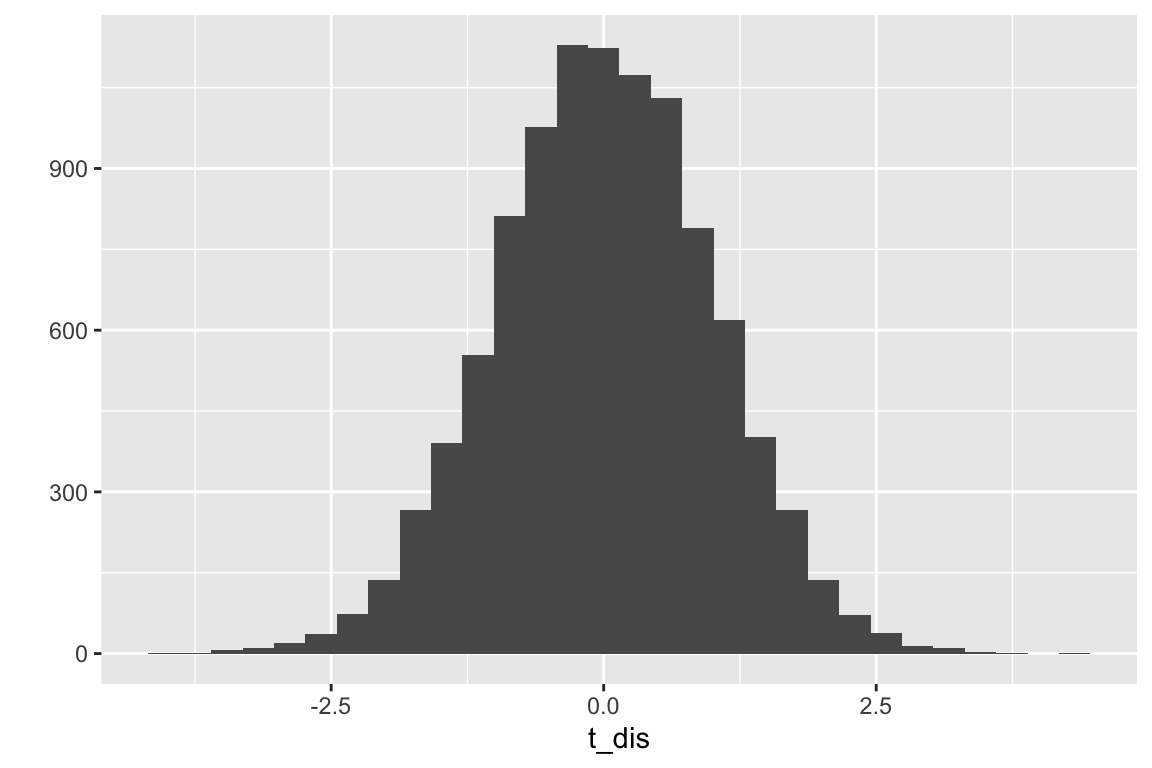
\includegraphics{Walker-elementary-statistical-modeling-draft_files/figure-latex/null-distribution-t-1.pdf}
\caption{\label{fig:null-distribution-t}Null distribution of t-values. The
simulation generated 100,000 t-tests with a true null.}
\end{figure}

Hey that looks pretty good! A \(p\) value can be computed by counting
the number of simulated \(t\)-values, \emph{including the observed
value}, that are more extreme (in either the positive or negative
direction) than the observed \(t\). Including the observed \(t\), there
are 10904 values that are more extreme than that observed. An
approximate measure of \(p\) is this count divided by 100,001 (why is 1
added to the denominator?), which is 0.1090389. This simulation-based
\(p\)-value is very (very!) close to that computed from the observed
\(t\)-test.

\subsection{P-values from the perspective of
permutation}\label{p-values-from-the-perspective-of-permutation}

A very intuitive way to think about \(p\)-values is with a permutation
test. Consider two of the treatment levels in the vole data, say vitamin
E and the vitamin C (I'm bored with the control!). Think about the
structure of the dataset: there are two columns, ``Treatment'', which
contains the assigned treatment, and ``Lifespan''. The values in the
Treatment column were randomly assigned prior to the start of the
experiment. If there is an effect of treatment on lifespan, then
assginment matters -- the values in the lifespan column for the vitamin
E rows will be more or less, on average, than the values in the lifepan
column for the vitamin C rows. Or, the lifespan values are what they are
\emph{because} of the values in the treatment column.

Now let's leave the values in the treatment column be, and just randomly
re-arrange or permute the lifespan values. What is the new expected
diference in lifespan between the two treatments? Zero, of course! That
is, because the lifespans were randomly re-arranged, they cannot be
caused by treatment assignment!

A permutation is a random re-arrangement of values in a column. Consider
the many thousands of permutations of the values in the lifespan column.
A difference in means can be computed from each of these permuations and
a distribution of differences can be generated. Is the observed
difference extreme relative to the other values in this distribution?
This is a permutation test -- it compares an observed statistic to a
distributin of the statistic computed over many thousands of
permutations.

\section{Statistical modeling instead of hypothesis
testing}\label{statistical-modeling-instead-of-hypothesis-testing}

This chapter is an introduction to a \(p\)-value by way of \(t\)-tests.
I advocate that you analyze \(t\)-test like questions using statistical
modeling instead of null hypothesis significance testing. The reason is
that we learn much more from an estimate of the effect and a CI than
from a \(t\) and \(p\)-value. But, it is also good to know that a \(t\)
test is a special case of a linear model, and you can get that \(t\) and
\(p\) using a statistical modeling approach should your boss want them
(and you cannot convince them otherwise). Let's explore this.

\begin{enumerate}
\def\labelenumi{\arabic{enumi}.}
\tightlist
\item
  Using the emmeans package, compute the effects (differences in means)
  of vitamin E and vitamin C on lifespan, relative to the control, with
  their 95\% CI and the \(t\) and \(p\) values for the cold-reared vole
  data.
\item
  Compute a separate \(t\)-test of vitamin-E vs.~control and vitamin C
  vs.~control.
\end{enumerate}

Are the \(t\) and \(p\) values the same? No! The reason is that the
statistical model had three groups and the SE of the difference was
computed from the sample standard deviation of all three groups. Each
t-test computes the SE of the difference from only the two groups being
compared. In general, the SE computed from all three groups is better
because it uses more information. This is one reason to prefer the
linear model instead of the separate t-tests.

\begin{enumerate}
\def\labelenumi{\arabic{enumi}.}
\setcounter{enumi}{2}
\item
  To convince yourself that a \(t\)-test is a special case as of a
  linear model, compute the effects of the vitamin E treatment (relative
  to control) \textbf{but exclude the vitamin C data from the model
  fit}. Now compare the \(t\) and \(p\) values with the \(t\)-test.
  These should be the same.
\item
  Now use the default t.test function by deleting ``var.equal=TRUE''
  from the function. Are \(t\) and \(p\) still equal to those from the
  statistical model? No! the reason is because the default t.test
  function uses a modification of the t-test called ``Welsch's t-test''.
  This test allows for heterogenity of variances. Several sources argue
  that one should always uses Welsch's test since it simplifies to the
  classical t-test when the sample variances are equal. This is true,
  but only relevant if you're into \(t\)-tests. And, we can model
  heterogenous variances using a statistical model. We'll do this in a
  later chapter.
\item
  Use the function \texttt{pairwise.t.test} to compute all pairwise
  t.tests among the three treatment levels. Is the \(p\)-value for the
  vitamin\_E - control contrast the same as that if using t.test (with
  var.equal=TRUE) or the statistical model with vitamin\_C data
  excluded? No! The reason is that pairwise.t.test adjusts the p-values
  for multiple testing as a default.
\end{enumerate}

Pro tip: Before you use a new R function like t.test or pairwise.t.test,
it is really advisable to read the help page and look at the defaults
for the parameters! Researchers publish errors because they failed to
look closely at what the R function was doing and they think the
function is doing something else. Ooops!

\section{frequentist probability and the interpretation of
p-values}\label{frequentist-probability-and-the-interpretation-of-p-values}

\subsection{Background}\label{background}

There are at least three different meanings of \textbf{probability}.

\begin{enumerate}
\def\labelenumi{\arabic{enumi}.}
\item
  \textbf{subjective probability} is the probability that an individual
  assigns to an event based on prior knowledge and the kinds of
  information considered reliable evidence. For example, if I asked a
  sample of students, what is the probability that a 30c homeopathic
  medicine could clear a \emph{Streptococcus} infection from your
  respiratory system, their answers would differ because of variation in
  their knowledge of basic science, including chemistry and physics,
  their knowledge of what homeopathic medicines are, and how they weight
  different kinds of evidence.
\item
  \textbf{classical probability} is simply one divided by the number of
  possible unique events. For example, with a six-sided die, there are
  six possible unique events. The probability of rolling a 2 is
  \(\frac{1}{6}\) and the probability of rolling an odd number is
  \(\frac{1}{2}\).
\item
  \textbf{frequentist probability} is based on the concept of
  \textit{long run frequency}. If I roll a die 10 times, the frequency
  of rolling a 2 will be approximately \(\frac{1}{6}\). If I roll the
  die 100 times, the frequency of rolling a two will be closer, but to
  \(\frac{1}{6}\). If I roll the die 1000 times, the frequency of
  rolling the die will be even closer to \(\frac{1}{6}\). So the
  frequentist definition is the expected frequency given an infinite
  number of rolls. For events with continous outcomes, a frequentist
  probability is the long run frquency of \emph{observing the outcome or
  one more extreme}.
\end{enumerate}

\subsection{\texorpdfstring{This book covers frequentist approaches to
statistical modeling and when a probability arises, such as the
\(p\)-value of a test statistic, this will be a frequentist
probability.}{This book covers frequentist approaches to statistical modeling and when a probability arises, such as the p-value of a test statistic, this will be a frequentist probability.}}\label{this-book-covers-frequentist-approaches-to-statistical-modeling-and-when-a-probability-arises-such-as-the-p-value-of-a-test-statistic-this-will-be-a-frequentist-probability.}

When we do a \(t\)-test, we get a \(p\)-value. There are several ways to
think about this probability. The most compact way is
\(P(data | null)\), which is literally read as the probability of the
data given the null (or ``conditional'' on the null), but is really
short for \emph{the probability of the data, or something more extreme
than the data, given that the null hypothesis is true}. The
``probability of the data'' is kinda vague. More specifically, we mean
the probability of some statistic about the data such as the difference
in means between group A and group B or the \(t\)-value associated with
this difference. So, a bit more formally, the probability returned in a
\(t\)-test is \(\mathrm{prob}(t \ge t_{obs} | H_0)\). This is the long
run frequency of observing a \(t\)-value as big or bigger than the
observed \(t\)-value (the one you actually got with your data) if the
null is true. Let's parse this into ``long run frequency of observing a
\(t\)-value as big or bigger than the observed \(t\)-value'' and ``null
is true''.

A thought experiment: You open a google sheet and insert 12 standard,
normal random deviates (so the true mean is zero and the true variance
is one) in Column A, rows 1-12. You arbitrarily assign the first six
values (rows 1-6) to treatment A and the second six values (rows 7-12)
to treatment B. You use the space immediately below these data to
compute the mean of treatment A, the mean of treatment B, the difference
in means (A - B), and a \(t\)-value. Unfortunately, google sheets
doesn't have a \(t\)-value function so you'd have to compute this
yourself. Or not, since this is a thought experiment. Now ``fill right''
or copy and paste these functions into 999 new columns. You now have
1000 \(t\) tests. The expected value of the difference in means is zero
(why?) but the actual values will form a normal distribution about zero.
Most will be close to zero (either in the negative or positive
direction) but some will be further from zero. The expected \(t\)-value
will also be zero (why?) and the distribution of these 1000 \(t\) values
will look normal but the tails are a little fuller. This row of \(t\)
values is a null distribution, because in generating the data we used
the exact same formula for the values assigned to A and the values
assigned to B. Now think of a \(t\)-value in your head, say 0.72
(remember that \(t\) values will largely range from about -3 to +3
although the theoretical range is \(-\infty\) to \(+\infty\). What is
the probability of observing a \(t\) of 0.72 \emph{or bigger} if the
null is true? Look at the row of \(t\)-values! Count the number of
\(t \ge 0.72\) and then divide by the total number of \(t\)-values in
the row (1000) and you have a probability computed as a frequency. But
remember the frequentist definition is the long run frequency, or the
expected frequency at the limit (when you've generated not 1000 or even
1,000,000 but an infinite number of columns and \(t\)-values).

Some asides to the thought experiment: First, why ``as big or bigger''
and not just the probability of the value itself? The reason is that the
probability of finding the exact \(t\) is 1/infinity, which doesn't do
us much good. So instead we compute the probability of finding \(t\) as
big, or bigger, than our observed \(t\). Second, the \(t\)-test
probability described above is a ``one-tail probability''. Because a
difference can be both in the positive direction and the negative
direction, we usually want to count all the \(t \ge 0.72\) and the
\(t \le -0.72\) and then add these two counts to compute the frequency
of \emph{as extreme or more extreme} values. This is called a
``two-tailed probability'' because we find extremes at both tails of the
distribution. Third, we don't really count \(t \ge 0.72\) but take
advantage of the beautiful mathematical properties of the theoretical
\(t\) distribution, which allows us to compute the frequentist
probability (expected long range frequency) given the \(t\)-value and
the degrees of freedom using the \(t\)-distribution.

Now what do I mean with the phrase ``null is true''? Most people equate
``null is true'' with ``no difference in means'' but the phrase entails
much more than this. Effectively, the phrase means that the \(p\)-value
is based on modeling the real data with a theoretical sample in which
all the points were randomly sampled from the same distribution and that
the assignment of the individual points to treatment was random. This
model means the theoretical sample has three properties: First, random
assignment to treatment after sampling from the same distribution means
that the expected means are the same, or put differently, the expected
difference in means between the assigned groups is zero. Second, random
assignment to treatment after sampling from the same distribution
\emph{also} means that the expected variances of the two groups are
equal. And third, random sampling means that the values of each point
are independent -- we cannot predict the value of one point knowing
information about any other point. \textbf{Here is what is super
important about this}: if we get a really low \(p\)-value, any one of
these consequences may be untrue about our data, for example it could be
that the true means of the two treatment groups really are different, or
it could mean it is the variances that differ between the two groups, or
it could mean that the data (or technically, the errors) are not
independent of each other. This is why we need certain assumptions to
make a \(p\)-value meaningful for empirical data. By assuming
independent error and homogenous (equal) variances in our two samples, a
low \(p\) value is evidence of unequal means.

\subsection{\texorpdfstring{Two interpretations of the
\(p\)-value}{Two interpretations of the p-value}}\label{two-interpretations-of-the-p-value}

Since we want to be working scientists who want to use \(p\)-values as a
tool, we need to know how to interpret (or use) the \(p\)-value to make
reasonable inferences and how to avoid mis-interpreting the \(p\)-value
and making unreasonable or even incorrect inferences. Ronald Fisher, the
inventor of frequentist statistics, developed an interpretation of the
\(p\)-value that is probably most useful for academic and applied
research programs. Neyman and Pearson (Neyman-Pearson) gave the
\(p\)-value a different interpretation, one that is probably most useful
for industrial quality control. Today's biology researchers use an
interpretation that is an odd hybrid of the two, which often leads to
silly inference. Regardless, understanding the distinction between
Fisher and Neyman-Pearson will inform how we write up our results in a
manuscript. I'll describe these in the context of the two-sample
\(t\)-test.

\subsubsection{Fisher's interpretation}\label{fishers-interpretation}

Fisher was working in the context of an agricultural field station, the
goal of which is to discover better agricultural practices. Does this
new fertilizer work better than our old fertilizer? This is the context
of much of modern biosciences and clinical medicine. Fisher thought of
\(p\) as evidence against the null; the smaller the \(p\) the better the
evidence that the means differ, which, in an experimental context,
implies a treatment effect. If an experiment results in a large
\(p\)-value, we can move on and test other fertilizers. If an experiment
results in a small \(p\)-value, we want to pursue this new fertilizer
more. Do more experiments! Fisher never thought of a single experiment
as definitive. The decision to move on or pursue is only partly informed
by the \(p\)-value and Fisher offered no rule about what \(p\)-value
lies on the threshold of this decision. When pressed, Fisher might say
that \(p=0.05\) is a reasonable threshold.

\subsubsection{Neyman-Pearson
interpretation}\label{neyman-pearson-interpretation}

Neyman-Pearson thought of \(p\) as the necessary and sufficient
information to make a decision between accepting the null (or at least
not rejecting the null) or rejecting the null and accepting an
alternative hypothesis. This decision balances two sorts of errors: Type
I (false positives), which they called \(\alpha\), and Type II (false
negatives), which they called \(\beta\). A false positive means the null
was rejected but there really is no effect. A false negative means that
the null was not rejected but there actually is an effect. \(\alpha\) is
set by the experimenter and is the long-term frequency (or ``rate'') of
false positives \textbf{when the null is true} that the experimenters
are willing to accept. This is easily understood in the context of
manufacturing. I've just made a batch of beer that I now need to ship. I
sample 10 cans and test the quality against a norm. If \(p < \alpha\),
we reject the null in favor of the alternative -- something may be wrong
with the batch, it differs from the norm. We throw the beer away. If
\(p > \alpha\), we do not reject the null, nor the beer! We ship it.

After setting \(\alpha\), the experimenter designs the experiment to
achieve an acceptable rate of \(\beta\). Since \(\beta\) is the false
negative rate then \(1-\beta\) is the rate of not making a false
negative error, that is, the rate of rejecting the null when there
really is an effect. This is called the \textbf{power} of the
experiment. An experiment with high power will have a low probability of
a Type II error. An experiment with low power will have a high
probability of a Type II error. Power is partly determined by sample
size, the bigger the sample the smaller the \(p\)-value, all other
things equal (think about why in the context of the formula for the
\(t\)-value). Power is also a function of \(\alpha\). If we set a low
\(\alpha\) (say, \(\alpha=0.01\)), the test is conservative. We are more
likely to fail to reject the null even if the null is false. This is the
balance. We want to make sure that we test our batch of beer using
enough cans to find a bad batch if it exists, but we don't want to test
too many cans because this is a waste of money. An experimenter sets
\(\alpha\), computes the sample size needed to achieve a certain level
of power (\(1-\beta\)), and then does the experiment.

In Fisher's interpretation, there is no \(\alpha\), no \(\beta\), no
alternative hypothesis, and no sharp decision rule. Instead, in Fisher,
\(p\) is a continuous measure of evidence against the null and its value
is interpreted subjectively by an informed and knowledgeable expert
using additional information to make decisions. Neyman-Pearson rejected
Fisher's conception of \(p\) as evidence against the null and used \(p\)
as a tool to make a decision that maintains long-term type I error rates
at alpha given a certain power. In Neyman-Pearson, \(p\) is compared to
a threshold, \(\alpha\) and this alone makes the decision. In
Neyman-Pearson, \(p\) is not treated as continuous information.
\(p=0.00000001\) is no more evidence to use to reject the null than
\(p=0.049\).

\subsection{NHST}\label{nhst}

Modern researchers interpret \(p\) using a combination of Fisher and
Neyman-Pearson concepts in what has become known as Null Hypothesis
Significance Testing (NHST). Similar to Neyman-Pearson, a \(p\)-value is
compared to \(\alpha\) but similar to Fisher, many researchers, and many
textbooks and statistics software (including base R) trichtomize a
statistically significant \(p\) into ``significance levels'' (three
asterisks for \(p < 0.001\), two asterisks for \(0.001 < p < 0.01\), and
one asterisk for \(0.01 < p < 0.05\)) but many researchers also
casuallly partition non-significant \(p\) values into ``marginally
signifiant'' (or similar) and ``not significant''.

\subsection{\texorpdfstring{Some major misconceptions of the
\(p\)-value}{Some major misconceptions of the p-value}}\label{some-major-misconceptions-of-the-p-value}

Setting the type I error rate \(\alpha\) to 0.05 is so pervasive that
I'm going to simply use ``0.05'' instead of ``alpha'' in discussing
misconceptions.

\subsubsection{\texorpdfstring{Misconception: \(p\) is the probability
that the null is true \emph{and} \(1-p\) is probability that the
alternative is
true}{Misconception: p is the probability that the null is true and 1-p is probability that the alternative is true}}\label{misconception-p-is-the-probability-that-the-null-is-true-and-1-p-is-probability-that-the-alternative-is-true}

Many researchers believe that if \(p > 0.05\) then ``there is no
effect.'' A frequentist hypothesis test cannot show that an effect
doesn't exist, only that the null has a low probablity of producing a
test statistic as extreme or more extreme than the observed effect.

Many researchers believe that if \(p < 0.05\) then ``there is an
effect.'' Again, a frequentist hypothesis test cannot show that an
effect exists, only that the null has a low probablity of producing a
test statistic as extreme or more extreme than the observed effect.

\begin{enumerate}
\def\labelenumi{\arabic{enumi}.}
\tightlist
\item
  The statement ``There is no effect of predators on feeding behavior''
  is not a valid conclusion of a frequentist hypothesis test.
\item
  The statement ``We found no effect of predators on feeding behavior''
  is misleading because a frequentist hypothesis test can neither find
  an effect nor find no effect.
\end{enumerate}

The two errors above are gross misconceptions that are pervasive in the
biology literature. A more subtle issue is the belief that a low
\(p\)-value shows that the researcher's explanatory hypothesis is
correct. For example, researchers believe the result ``the prey fish fed
14.2 (95\% CI: 9.2, 19.2) minutes shorter in the presence of the
predator fish'' confirms their hypothesis that prey modulate feeding
duration as a function of their ability to assess the risk of predation.
Some alternative explanations:

\begin{enumerate}
\def\labelenumi{\arabic{enumi}.}
\tightlist
\item
  The predator fish also competes with the prey fish for the prey fish's
  food and with less food the prey fish spends less time feeding because
  it gives up when food density drops below some amount.
\item
  The predator fish is introduced to the prey tank by hand and odorant
  molecules from the researcher's hands are detected by the prey and the
  prey reduces feeding duration because of these odorants.
\end{enumerate}

Importantly, no single experiment confirms an explanatory hypothesis.
Instead, alternative explanations require multiple experiments with
different controls to ``rigrously probe'' the preferred hypothesis.

\subsubsection{\texorpdfstring{Misconception: a \(p\)-value is
repeatable}{Misconception: a p-value is repeatable}}\label{misconception-a-p-value-is-repeatable}

Many researchers believe that a \(p\)-value is a precise measure -- that
if the experiment were replicated, a similar \(p\) would result. This
belief requires at least two misconceptions. First, if the null were
true, then \emph{any} \(p\)-value is equally likely. \(p=0.00137\) is
just as likely as \(p=0.492\). In other words, if the null were true,
the \(p\)-value is not replicable at all! Second, the \(p\) value is
highly dependent on the sample, and can be highly variable among
replications, but there is no true \(p\)-value, so there can be no
estimate or standard error. Let's explore these.

\textbf{What is the distribution of \(p\)-values under the null?} I
often ask students, ``if the null were true, what is the most likely
\(p\)-value?'' or ``if the null were true, what kind of \(p\)-values
would we expect, that is what is the expected distribution''. A common
answer is \(p=0.5\) is the most likely value and something like a normal
curve, except the tails abruptly stop at 0 and 1, is the expected
distribution.

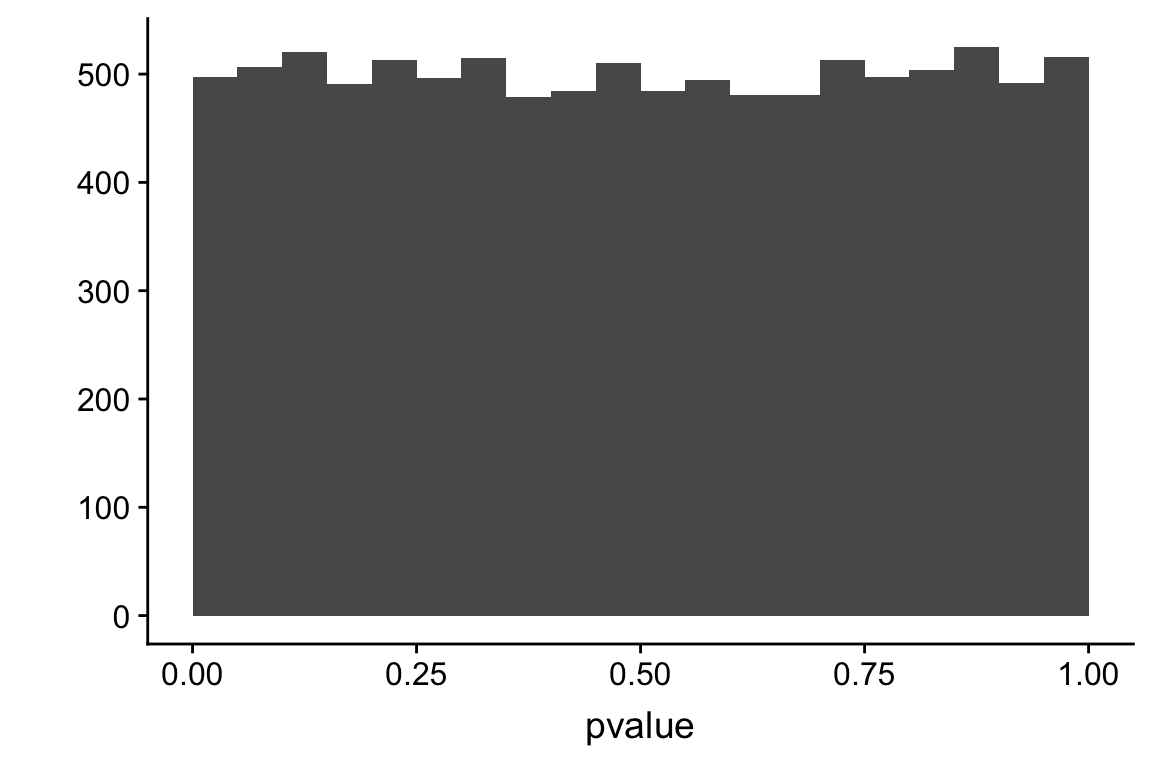
\includegraphics{Walker-elementary-statistical-modeling-draft_files/figure-latex/uniform-1.pdf}

\textbf{The incredible inconsistency of the \(p\)-value}

How replicable is the conclusion of an experiment if the \(p\)-value for
a \(t\)-test is 0.03? If our conclusion is based on \(p < 0.05\), then
the conclusion is not very replicable. The simulation below shows the
results of 15 replicates of an experiment with true power of 40\%. There
are five ``significant'' results (one less than expected) but several
replicates have very high \(p\)-values.

\begin{figure}
\centering
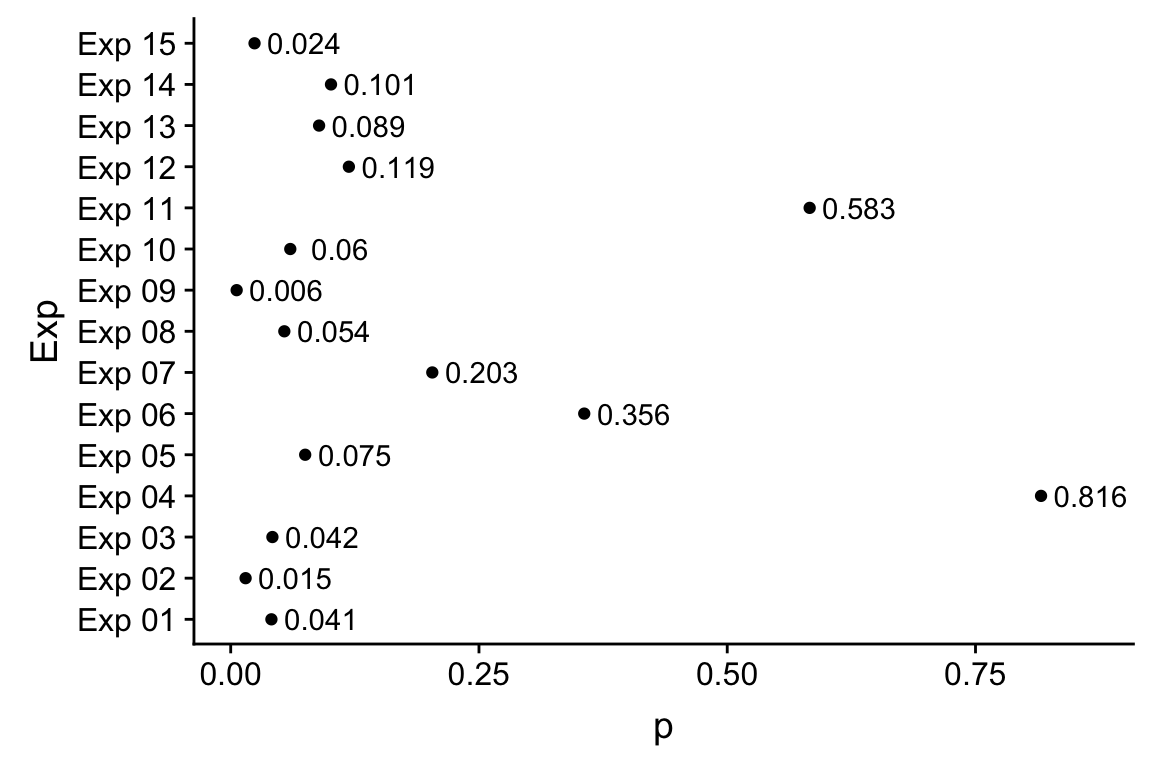
\includegraphics{Walker-elementary-statistical-modeling-draft_files/figure-latex/dance-fig-1.pdf}
\caption{\label{fig:dance-fig}Variability of \(p\)-values when the power is
0.4}
\end{figure}

\subsubsection{Misconception: 0.05 is the lifetime rate of false
discoveries}\label{misconception-0.05-is-the-lifetime-rate-of-false-discoveries}

An important and widespread misconception is that if a researcher
consistently uses \(\alpha=0.05\), then the frequency of incorrectly
concluding an effect exists, or ``discovering'' an effect, over the
lifetime of the researcher, will be 5\%. This is incorrect. This ``false
discovery rate'' is the frequency of false positives divided by the
frequency of positives (the sum of false and true positives). This
differs from the the Type I error rate, which is the frequency of false
positives divided by the frequency of tests \emph{in which the null is
true}.

Imagine we test

\begin{enumerate}
\def\labelenumi{\arabic{enumi}.}
\tightlist
\item
  1000 null hypotheses over a lifetime
\item
  60\% are true nulls, this means there are 600 true nulls and 400 true
  effects
\item
  alpha is 5\%. This means we expect to find \(p \le 0.05\) 30 times
  (\(0.05 \times 600\)) when the null is true
\item
  power is 25\%. This means we expect to find \(p \le 0.05\) 100 times
  (\(0.25 \times 400\)) when the null is false
\item
  We have made \(30 + 100=130\) ``discoveries'' (all experiments with
  \(p \le 0.05\)), but
\item
  30 of the 130, or 23\%, are ``false discoveries''.
\end{enumerate}

That is 11.7\% is the ``false discovery rate''.

Think about this. If the null is never true, you cannot have a false
discovery--every \(p \le 0.05\) is a true discovery (the false discovery
rate is 0\%). And if the null is always true, every \(p < 0.05\) is a
false discovery (the false discovery rate is 100\%).

\subsubsection{\texorpdfstring{Misconception: a low \(p\)-value
indicates an important
effect}{Misconception: a low p-value indicates an important effect}}\label{misconception-a-low-p-value-indicates-an-important-effect}

Many researchers write results as if they believe that a small
\(p\)-value means the effect is big or important. This may misconception
may arise because of the ubiquitous use of ``significant'' to indicate a
small p-value and ``very'' or ``extremely'' or ``wicked'' significant to
indicate a really small p-value. Regardless, this is a misconception. A
small p-value will usually result when there is high power (but can
occur even if power is low) and power is a function of effect size,
variability (the standard deviation), and sample size. A small \(p\)
could result from a large effect size but can also result with a small
effect size if the sample size is big enough.

This is easy to simulate (see script below). Let's model the effect of
the genotype of a gene on height

\begin{Shaded}
\begin{Highlighting}[]
\KeywordTok{set.seed}\NormalTok{(}\DecValTok{1}\NormalTok{)}
\NormalTok{rho <-}\StringTok{ }\FloatTok{0.5}
\NormalTok{n <-}\StringTok{ }\DecValTok{10}\OperatorTok{^}\DecValTok{4}
\NormalTok{genotype <-}\StringTok{ }\KeywordTok{c}\NormalTok{(}\StringTok{"+/+"}\NormalTok{, }\StringTok{"+/-"}\NormalTok{, }\StringTok{"-/-"}\NormalTok{)}
\NormalTok{Sigma <-}\StringTok{ }\KeywordTok{diag}\NormalTok{(}\DecValTok{2}\NormalTok{)}
\NormalTok{Sigma[}\DecValTok{1}\NormalTok{,}\DecValTok{2}\NormalTok{] <-}\StringTok{ }\NormalTok{Sigma[}\DecValTok{2}\NormalTok{,}\DecValTok{1}\NormalTok{] <-}\StringTok{ }\NormalTok{rho}
\NormalTok{X <-}\StringTok{ }\KeywordTok{rmvnorm}\NormalTok{(n, }\DataTypeTok{mean=}\KeywordTok{c}\NormalTok{(}\DecValTok{0}\NormalTok{,}\DecValTok{0}\NormalTok{), }\DataTypeTok{sigma=}\NormalTok{Sigma)}
\KeywordTok{colnames}\NormalTok{(X) <-}\StringTok{ }\KeywordTok{c}\NormalTok{(}\StringTok{"X1"}\NormalTok{, }\StringTok{"X2"}\NormalTok{)}
\NormalTok{beta <-}\StringTok{ }\KeywordTok{c}\NormalTok{(}\FloatTok{0.05}\NormalTok{, }\FloatTok{0.05}\NormalTok{)}
\NormalTok{y <-}\StringTok{ }\NormalTok{X}\OperatorTok\NormalTok{beta }\OperatorTok{+}\StringTok{ }\KeywordTok{rnorm}\NormalTok{(n)}
\NormalTok{fit <-}\StringTok{ }\KeywordTok{lm}\NormalTok{(y }\OperatorTok{~}\StringTok{ }\NormalTok{X)}
\KeywordTok{coefficients}\NormalTok{(}\KeywordTok{summary}\NormalTok{(fit))}
\end{Highlighting}
\end{Shaded}

\begin{verbatim}
##                Estimate Std. Error   t value     Pr(>|t|)
## (Intercept) 0.007472959 0.01007946 0.7414046 4.584656e-01
## XX1         0.044304824 0.01154709 3.8368830 1.253725e-04
## XX2         0.048228101 0.01170855 4.1190490 3.835033e-05
\end{verbatim}

\subsubsection{\texorpdfstring{Misconception: a low \(p\)-value
indicates high model fit or high predictive
capacity}{Misconception: a low p-value indicates high model fit or high predictive capacity}}\label{misconception-a-low-p-value-indicates-high-model-fit-or-high-predictive-capacity}

On page 606, of Lock et al ``Statistics: Unlocking the Power of Data'',
the authors state in item D ``The p-value from the ANOVA table is 0.000
so the model as a whole is effective at predicting grade point
averages.'' This is incorrect. A p-value is not a measure of the
predictive capacity of a model because the p-value is a function of 1)
signal, 2) noise (unmodeled error), and 3) sample size while predictive
capacity is a function of the signal:noise ratio. If the signal:noise
ratio is tiny, the predictive capacity is small but the p-value can be
tiny if the sample size is large. This is easy to simulate (see script
below). The whole-model p-value is exceptionally small (0.00001002) but
the relative predictive ability, measured by the \(R^2\), is near zero
(0.002).

\begin{Shaded}
\begin{Highlighting}[]
\KeywordTok{library}\NormalTok{(mvtnorm)}
\KeywordTok{set.seed}\NormalTok{(}\DecValTok{1}\NormalTok{)}
\NormalTok{rho <-}\StringTok{ }\FloatTok{0.5}
\NormalTok{n <-}\StringTok{ }\DecValTok{10}\OperatorTok{^}\DecValTok{4}
\NormalTok{Sigma <-}\StringTok{ }\KeywordTok{diag}\NormalTok{(}\DecValTok{2}\NormalTok{)}
\NormalTok{Sigma[}\DecValTok{1}\NormalTok{,}\DecValTok{2}\NormalTok{] <-}\StringTok{ }\NormalTok{Sigma[}\DecValTok{2}\NormalTok{,}\DecValTok{1}\NormalTok{] <-}\StringTok{ }\NormalTok{rho}
\NormalTok{X <-}\StringTok{ }\KeywordTok{rmvnorm}\NormalTok{(n, }\DataTypeTok{mean=}\KeywordTok{c}\NormalTok{(}\DecValTok{0}\NormalTok{,}\DecValTok{0}\NormalTok{), }\DataTypeTok{sigma=}\NormalTok{Sigma)}
\KeywordTok{colnames}\NormalTok{(X) <-}\StringTok{ }\KeywordTok{c}\NormalTok{(}\StringTok{"X1"}\NormalTok{, }\StringTok{"X2"}\NormalTok{)}
\NormalTok{beta <-}\StringTok{ }\KeywordTok{c}\NormalTok{(}\FloatTok{0.05}\NormalTok{, }\OperatorTok{-}\FloatTok{0.05}\NormalTok{)}
\NormalTok{y <-}\StringTok{ }\NormalTok{X}\OperatorTok\NormalTok{beta }\OperatorTok{+}\StringTok{ }\KeywordTok{rnorm}\NormalTok{(n)}
\NormalTok{fit <-}\StringTok{ }\KeywordTok{lm}\NormalTok{(y }\OperatorTok{~}\StringTok{ }\NormalTok{X)}
\KeywordTok{summary}\NormalTok{(fit)}
\end{Highlighting}
\end{Shaded}

\begin{verbatim}
## 
## Call:
## lm(formula = y ~ X)
## 
## Residuals:
##     Min      1Q  Median      3Q     Max 
## -3.6449 -0.6857  0.0148  0.6756  3.6510 
## 
## Coefficients:
##              Estimate Std. Error t value Pr(>|t|)    
## (Intercept)  0.007473   0.010079   0.741 0.458466    
## XX1          0.044305   0.011547   3.837 0.000125 ***
## XX2         -0.051772   0.011709  -4.422  9.9e-06 ***
## ---
## Signif. codes:  0 '***' 0.001 '**' 0.01 '*' 0.05 '.' 0.1 ' ' 1
## 
## Residual standard error: 1.008 on 9997 degrees of freedom
## Multiple R-squared:  0.0023, Adjusted R-squared:  0.002101 
## F-statistic: 11.52 on 2 and 9997 DF,  p-value: 1.002e-05
\end{verbatim}

\paragraph{\texorpdfstring{What the \(p\)-value does not
mean}{What the p-value does not mean}}\label{what-the-p-value-does-not-mean}

\begin{enumerate}
\def\labelenumi{\arabic{enumi}.}
\tightlist
\item
  \(p\) is not the probability of the null being true. More formally,
  this probability is \(P(null | data)\) but our \(p\)-value is
  \(P(data | null)\). These are not the same. \(P(null | data)\) is the
  probability of the null being true given the data. \(P(data | null)\)
  is the probability of our data, or something more extreme than our
  data, conditional on a true null.
\item
  \(1-p\) is not the probability of the alternative
\item
  \(p\) is not a measure of effect size.
\item
  \(p\) in one experiment is not the same level of evidence against the
  null as in another experiment
\item
  \(p\) is not a great indicator of which is more likely, H0 or H1.
\item
  If one treatment level has \(p < 0.05\) and another treatment level
  has \(p > 0.05\), this is not evidence that the treatment levels have
  different effects on the outcome.
\end{enumerate}

\subsection{Recommendations}\label{recommendations}

\textbf{If you are working on basic science research} simply report the
exact \(p\)-value, along with a CI. If \(p < 0.05\) (or some other
\(\alpha\)) do not report this as ``significant'' -- in fact, avoid the
word ``significant''. In the english language, ``significant'' implies
big or important. Small \(p\)-values can result even with trivially
small effects if \(n\) is big or sample variation is small. If \(p\) is
smaller than say 0.001, then this is pretty good evidence that the data
is not a fluke of sampling. But if \(p\) is closer to 0.01 or 0.05, this
is only weak evidence of a fluke because of the sampling variability of
\(p\).

\textbf{If you are working on quality control} then a \(p\) value is a
useful tool, but is only relevant compared to a decision rule with
well-reasoned values of \(\alpha\) and \(\beta\) -- exact values of
\(p\) are not very meaningful.

\section{Problems}\label{problems-2}

Problem 1 -- simulate the distribution of \(p\) under the null. There
are many ways to do this but a straightforard approach is to

\begin{enumerate}
\def\labelenumi{\arabic{enumi}.}
\tightlist
\item
  Create a \(2n \times m\) matrix of random normal deviates with mean 0
  and sd 1
\item
  Do a \(t\)-test on each column, with the first \(n\) values assigned
  to one group and the remaining \(n\) values assigned to the second
  group. Save the \(p\)-value from each.
\item
  Plot a histogram of the \(p\)-values.
\item
  What is the distribution? What is the most likely value of \(p\)?
\end{enumerate}

Problem 2 -- simulate power. Again, many ways to do this but following
up on Problem 1. 1. Create a \(2n \times m\) matrix of random normal
deviates with mean 0 and sd 1 2. Add an effect to the first \(n\) values
of each column. Things to think about a. what is a good effect size to
add? The effect/sd ratio, known as Cohen's d, is a relative (or
standardized) measure of effect size. Cohen suggest 0.2, 0.5, and 0.8 as
small, medium, and large standardized effects. b. should the same effect
be added to each individual? Yes! It is the random component that
captures the individual variation in the response. 3. Do a \(t\)-test on
each column of the matrix, using the first \(n\) values in group 1 and
the remaining \(n\) values in group 2. Save the p-values for each. 4.
Compute the power, the relative frequency \(p \le 0.05\). 5. Repeat with
different values of \(n\), effect size, and sd, but only vary one at a
time. How does power vary with these three parameters?

Problem 3 -- write a script for a permutation test of the vitamin E and
vitamin C levels of the vole data. Compare this to the \(t\)-test.

Problem 4 -- grad students only. Simulate the false discovery rate.
Explore the parameters: the frequency of true nulls and the power.

\chapter{\texorpdfstring{Two (or more) Categorical \(X\) -- Factorial
designs}{Two (or more) Categorical X -- Factorial designs}}\label{two-or-more-categorical-x-factorial-designs}

\section{Factorial experiments}\label{factorial-experiments}

A factorial experiment is one in which there are two or more categorical
\(X\) that are \textbf{crossed}, so the groups contain different
combinations of levels of each factor. Factorial experiments are used to
estimate the \textbf{interaction} between factors. Let's explore this
using data from xxx

The urchin data are from an experiment measuring the effect of \(Temp\)
and \(CO2\) on larval sea urchin metabolic rate (\(Resp\)) (there are
other outcome measures in the study too). The units of metabolic rate
are pmol O2/hr/larva. There are two \(Temp\) levels (13C and 18C) and
two \(CO2\) levels (400 µAtm and 1100) and the factors are crossed, so
this is a \(2 \times 2\) (crossed or factorial) design. There are
\(n=6\) replicates for each combination of the levels. A good way to
visualize the treatment combinations in a crossed design is with a
\(m \times p\) table showing all combinations of the \(m\) levels of
factor 1 (\(Temp\)) against the \(p\) levels of factor 2 (\(CO2\))

\begin{figure}
\centering
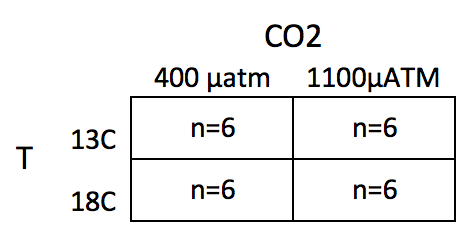
\includegraphics[width=0.50000\textwidth]{images/2x2_table.png}
\caption{The urchin experimental design as a 2 x 2 table}
\end{figure}

The upper left cell contains the 13C level with the Temperature factor
and the 400 µAtm level within the CO2 factor. The replicates in this
cell were grown with no added treatments, so this cell is the
``control'' for Temp and the control for CO2, which we will use as the
``reference'' group for the linear model. The replicates in the lower
left cell were grown with an added temperature treatment (in this case,
a 5 C higher temperature). The replicates in the upper right cell were
grown an added CO2 treatment (a 700 µATM higher CO2). And finally, the
replicates in the bottom right cell were grown with both the added
temperature (+5 C) and added CO2 (+700 µATM). Here, I use a ``+'' or
``-'' to designate the addition (or not) of the treatment, so our
\(2 \times 2\) treatment levels are Temp-/CO2-, Temp+/CO2-, Temp-/CO2+
and Temp+/CO2+.

\subsection{Model coefficients: an interaction effect is what is
leftover after adding the treatment effects to the
control}\label{model-coefficients-an-interaction-effect-is-what-is-leftover-after-adding-the-treatment-effects-to-the-control}

A factorial design allows a researcher to estimate the interaction
between two factors. To clarify this, let's fit the factorial model and
look at the coefficient table. The fit model is

\begin{equation}
Resp_i = b_0 + b_1 Temp^+ + b_2 CO2^+ + b_3 Temp^+ CO2^+ + e_i
\end{equation}

\% Again, \(Temp^+\) and \(CO2^+\) are dummy variables. The model also
includes \(Temp^+ CO2^+\), which is a dummy variable for the interaction
between Temp and CO2. The value of this interaction dummy variable is
literally the product of the two main factor dummy variables (\(Temp^+\)
and \(CO2^+\)), which can be verified with the model matrix (which here,
is computed from the subset of the data that includeds only the first
two rows of each treatment combination)

\begin{tabular}{r|r|r|r}
\hline
(Intercept) & Temp+ & CO2+ & Temp+:CO2+\\
\hline
1 & 0 & 0 & 0\\
\hline
1 & 0 & 0 & 0\\
\hline
1 & 1 & 0 & 0\\
\hline
1 & 1 & 0 & 0\\
\hline
1 & 0 & 1 & 0\\
\hline
1 & 0 & 1 & 0\\
\hline
1 & 1 & 1 & 1\\
\hline
1 & 1 & 1 & 1\\
\hline
\end{tabular}

The coefficient table is

\begin{tabular}{l|r|r|r|r}
\hline
  & Estimate & Std. Error & t value & Pr(>|t|)\\
\hline
(Intercept) & 8.23 & 0.73 & 11.3 & 0.000\\
\hline
Temp+ & 4.51 & 1.03 & 4.4 & 0.000\\
\hline
CO2+ & -0.32 & 1.03 & -0.3 & 0.761\\
\hline
Temp+:CO2+ & -2.68 & 1.45 & -1.9 & 0.079\\
\hline
\end{tabular}

The Intercept (\(b_0\)) is the mean (8.23) of the reference (Temp-/CO2-)
group, and so the mean of the upper left cell in Table 1). The Temp+
coefficient (\(b_1\)) is the estimate of the added temperature effect
relative to the reference, and so is the mean of the lower left cell
minus the mean of the upper left cell
(\(b_1=\bar{Y}_{Temp^+}-\bar{Y}_{-/-}\)). The CO2+ coefficient (\(b_2\))
is the estimate of the added CO2 effect relative to the reference, and
so is the mean of the upper right cell minus the mean of the upper left
cell (\(b_2=\bar{Y}_{CO2^+}-\bar{Y}_{-/-}\)). The Temp+:CO2+ coefficient
(\(b_3\)) is the estimate of the \textbf{interaction effect}, which is
the effect in addition to the Temp\(^+\) and CO2\(^+\) effects. If you
added \(b_1\) and \(b_2\) to \(b_0\), you would get the mean of the
Temp\(^+\)/CO2\(^+\) group \emph{if the effects were purely additive}.
So the interaction effect is the difference between the mean of the
bottom right cell and the sum of the coefficients of the other three
cells (\(b_3 = \bar{Y}_{Temp^+CO2^+} - (b0 + b1 + b2)\)). An interaction
is a \textbf{non-additive effect}. Think about this. Adding 5 C
increases respiration by 4.51 units. Adding 700 \(\mu\)ATM CO2 decreases
respiration by .32 units. If these effects were purely additive, then
adding both 5 C and 700 \(\mu\)ATM should result in a mean of 8.23 +
4.51 - .32 = 12.42 units for the Temp\(^+\)/CO2\(^+\) group. What is the
mean of this group?

9.74! So the difference between the ``additive expectation'' and the
actual mean is \(9.74 - 12.42 = -2.68\), which is the interaction effect
(coefficient).

\subsection{What is the biological meaning of an interaction
effect?}\label{what-is-the-biological-meaning-of-an-interaction-effect}

I can dead lift 150 pounds and my friend Jake can deadlift 175 pounds.
Working together, we should be able to lift 325 pounds. What if
together, we could actually lift 400 pounds? If this were the case, this
would be an interaction with an effect equal to 75 pounds. Is this
biologically plausible? If so, what is the mechanism? Here is a possible
mechanism (although I am highly skeptical of it having a magnitude of 75
pounds): when lifting an object as part of a group, the central nervous
system allows increased motor unit recruitment, and so each person can
lift more weight than they could if lifting alone. A positive
interaction like this is called \emph{synergistic}. Always think about
the biological meaning of an interaction effect.

\subsection{What about models with more than two
factors?}\label{what-about-models-with-more-than-two-factors}

A factorial model can have more than two factors, for example, a model
with three factors (A, B, and C), each with two levels (which I'll
designate with a ``+''), is

\begin{equation}
Y = \beta_0 + \beta_1 A^+ + \beta_1 B^+ + \beta_3 C^+ + \beta_4 A^+ B^+ + \beta_5 A^+ C^+ + \beta_6 B^+ C^+ + \beta_7 A^+ B^+ C^+ + \varepsilon
\end{equation}

It is easy enough to get an ANOVA table with \(p\)-values for this model
but I don't recommend it because

\begin{enumerate}
\def\labelenumi{\arabic{enumi}.}
\tightlist
\item
  If space and/or time and/or materials are limited then it typically
  makes more sense to prioritize the power to estimate standard errors
  by choosing one of the two-factor models and increasing sample size
\item
  Interaction effects in 2-factor models are hard enough to interpret. A
  3-way interaction is very, very tough to interpret. If all we did was
  table up \(F\)-ratios and \(p\)-values, this wouldn't matter. But it
  does matter.
\end{enumerate}

\subsection{The additive model}\label{the-additive-model}

Sometimes researchers fit reduced models. For example, the \(p\)-value
for the interaction effect in the full model is 0.079, which is not
statististically significant. This would lead some researchers to
explicitly conclude (mistakenly), that there is no interaction between
CO2 and Temp and that the effects of CO2 and Temp on metabolism are
\textbf{additive} (see below). This would lead others (controversially)
to refit the model excluding the interaction term:

\begin{equation}
Resp_i = b_0 + b_1Temp^+ + b_2CO2^+ + e_i
\end{equation}

\% This particular reduced model is often referred to as the
\textbf{additive model}, since it excludes the the interaction term,
which is a \emph{product} of other terms. Indeed, the title of the
urchin paper is ``Temperature and CO2 additively regulate physiology,
morphology and genomic responses of larval sea urchins,
\emph{Strongylocentrotus purpuratus}.'' It is important to recognize
that unless the interaction effect is precisely zero, the coefficients
of Temp+ and CO2+ will change. Here are the coefficients of the additive
model

\begin{tabular}{l|r|r|r|r}
\hline
  & Estimate & Std. Error & t value & Pr(>|t|)\\
\hline
(Intercept) & 8.90 & 0.66 & 13.4 & 0.000\\
\hline
Temp+ & 3.17 & 0.77 & 4.1 & 0.000\\
\hline
CO2+ & -1.66 & 0.77 & -2.2 & 0.042\\
\hline
\end{tabular}

For several reasons, one should not drop a term because \(p>0.05\).

\begin{enumerate}
\def\labelenumi{\arabic{enumi}.}
\tightlist
\item
  The \(p\)-value is an arbitrary dichotomization of a continuous
  variable. Would it make sense to behave differently if \(p=0.051\) vs.
  \(p=0.049\), given that these two p-values are effectively identical?
\item
  A \(p\)-value is not evidence that an effect is zero, or ``doesn't
  exist'', or event that an effect is ``trivially small''. This is
  because \(p\)-values are a function of measurement error, sampling
  error, and sample size, in addition to effect size.
\end{enumerate}

\subsection{Contrasts -- simple vs.~main
effects}\label{contrasts-simple-vs.main-effects}

In a \(m \times p\) design, there are \(mp\) cell means and, therefore,
\(mp(mp-1)/2\) pairwise contrasts. For the urchin data, these are

\begin{enumerate}
\def\labelenumi{\arabic{enumi}.}
\tightlist
\item
  Temp+/CO2- - Temp-/CO2- (bottom left - top left)
\item
  Temp+/CO2+ - Temp-/CO2+ (bottom right - top right)
\item
  Temp-/CO2+ - Temp-/CO2- (top right - top left)
\item
  Temp+/CO2+ - Temp+/CO2- (bottom right - bottom left)
\item
  Temp-/CO2+ - Temp+/CO2- (top right - bottom left)
\item
  Temp+/CO2+ - Temp-/CO2- (bottom right - top left)
\end{enumerate}

\begin{enumerate}
\def\labelenumi{(\arabic{enumi})}
\tightlist
\item
  and (2) are the \textbf{simple effects} of Temp at each level of CO2.
  (3) and (4) are the simple effects of CO2 at each level of Temp. (5)
  is the response of the CO2 treatment at the reference level of Temp
  minus the response of the Temp treatment at the reference level of
  CO2. This probably is not a very interesting contrast. (6) is the
  combined response of Temp and CO2, including the interaction, minus
  the control. This also is unlikely to be of much interest.
\end{enumerate}

\begin{tabular}{l|r|r|r|r|r|r|r}
\hline
contrast & estimate & SE & df & lower.CL & upper.CL & t.ratio & p.value\\
\hline
Temp+,CO2- - Temp-,CO2- & 4.51 & 1.03 & 20 & 2.4 & 6.7 & 4.4 & 0.000\\
\hline
Temp-,CO2+ - Temp-,CO2- & -0.32 & 1.03 & 20 & -2.5 & 1.8 & -0.3 & 0.761\\
\hline
Temp-,CO2+ - Temp+,CO2- & -4.83 & 1.03 & 20 & -7.0 & -2.7 & -4.7 & 0.000\\
\hline
Temp+,CO2+ - Temp-,CO2- & 1.51 & 1.03 & 20 & -0.6 & 3.6 & 1.5 & 0.157\\
\hline
Temp+,CO2+ - Temp+,CO2- & -3.00 & 1.03 & 20 & -5.1 & -0.9 & -2.9 & 0.008\\
\hline
Temp+,CO2+ - Temp-,CO2+ & 1.82 & 1.03 & 20 & -0.3 & 4.0 & 1.8 & 0.091\\
\hline
\end{tabular}

\textbf{Main effects} are contrasts between

\section{Reporting results}\label{reporting-results-2}

\subsection{Text results}\label{text-results}

The effect of the increased temperature at the control CO2 level was 4.5
(95\% CI: 2.4, 6.7; \(p < 0.001\)) pmol O2/hr/larva. The effect of
increased CO2 at the control temperature was -0.3 (95\% CI: -2.4, 1.8;
\(p=.76\)) pmol O2/hr/larva. The interaction effect was -2.7 (95\% CI:
-5.7, 0.3; \(p = 0.079\)) pmol O2/hr/larva. Because of the relatively
large interaction, the effect of temperature at the high level of CO2
was less than half the effect at the low level of CO2 (estimate: 1.82;
95\% CI: -0.3, 4.0; \(p = 0.091\)) and the effect of CO2 at the high
level of Temp was 10 times greater than that at the low level of Temp
(estimate: -3.0; 95\% CI: -5.1, -.9; \(p = 0.0084\)).

The CI on the interaction includes both large negative values and
trivially small values, including zero, and, consequently, our data is
compatible with both scientific models (that is, we can neither support
nor reject the predictions of the scientific model using these results).

\subsection{Harrellplot}\label{harrellplot}

If the focus is on the interaction, then a Harrell Plot of coefficients
is a good choice for communicating this.

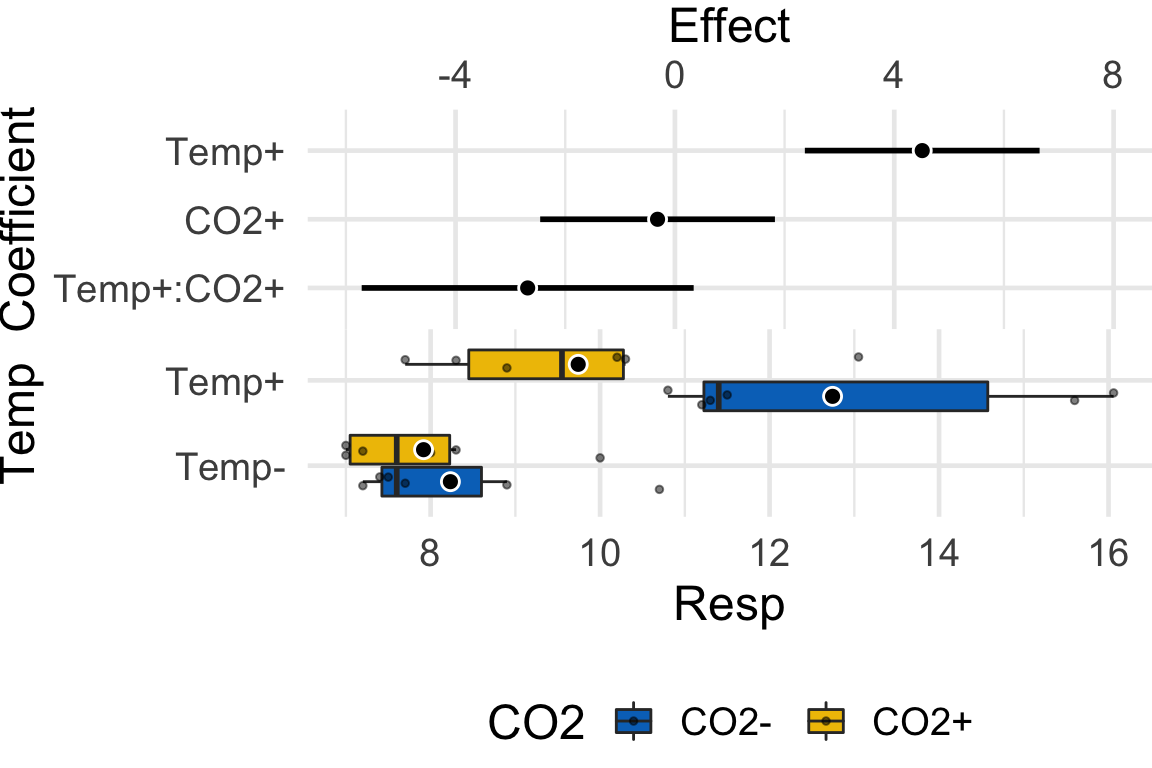
\includegraphics{Walker-elementary-statistical-modeling-draft_files/figure-latex/urchin-harrellplot1-1.pdf}

The plot shows that a relatively big and positive Temp effect, a
relatively small CO2 effect (and one with too much noise to have any
confidence of the sign) and a intermediate interaction effect. In the
original paper, the researchers were testing a scientific (not
statistical!) model that predicted no interaction, and the researchers
argued that these data support this model because of the small p-value
for this effect (see the table above). Well, the data do support that
model (one end of the 95\% CI for the interaction includes zero, and
other very small values) but they also support a model of a large
interaction (the other end of the 95\% CI includes large negative
effects). The data are too course (or the signal:noise ratio is to
small) to have much confidence in the size of the interaction effect.
Some comments:

\begin{enumerate}
\def\labelenumi{\arabic{enumi}.}
\tightlist
\item
  It is not valid to claim that an effect ``doesn't'' exist because p
  \textgreater{} 0.05 (see chapter xxx)
\item
  Researchers need to draw conclusions based on \emph{both} ends of the
  CI, as well as the mean!
\item
  A sample size of 6 will generally be very low power to get a precise
  estimate of the interaction unless the sampling variability is very
  small.
\end{enumerate}

If we are more interested in differences between the different treatment
combinations, then a Harrell plot with the contrasts is a good way to
communicate this.

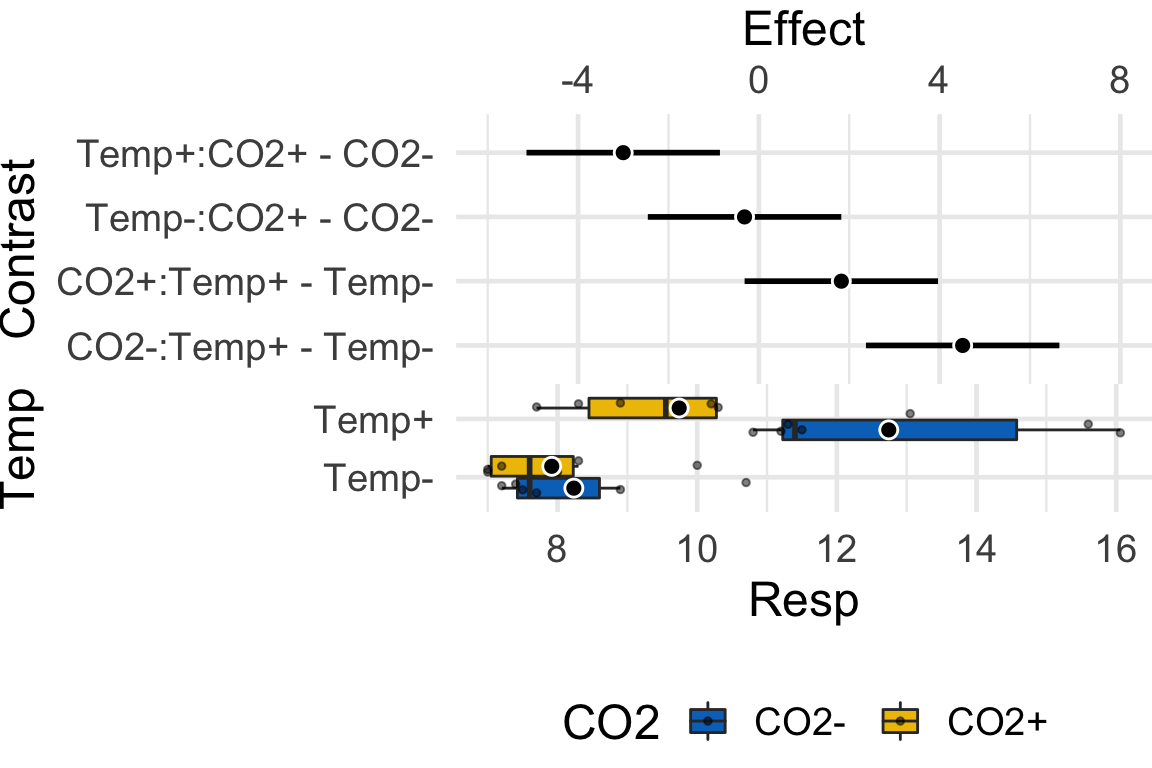
\includegraphics{Walker-elementary-statistical-modeling-draft_files/figure-latex/urchin-harrellplot2-1.pdf}
The four contrasts are differences between the means of pairs of cells
in the \(2 \times 2\) table:

\begin{enumerate}
\def\labelenumi{\arabic{enumi}.}
\tightlist
\item
  ``Temp+: CO2+ - CO2-'' -- lower right - lower left
\item
  ``Temp-: CO2+ - CO2-'' -- upper right - upper left
\item
  ``CO2+: Temp+ - Temp-'' -- lower right - upper right
\item
  ``CO2-: Temp+ - Temp-'' -- lower left - upper left
\end{enumerate}

\subsection{Interaction plots}\label{interaction-plots}

A common way to plot the results of the model is with an
\textbf{interaction plot}.

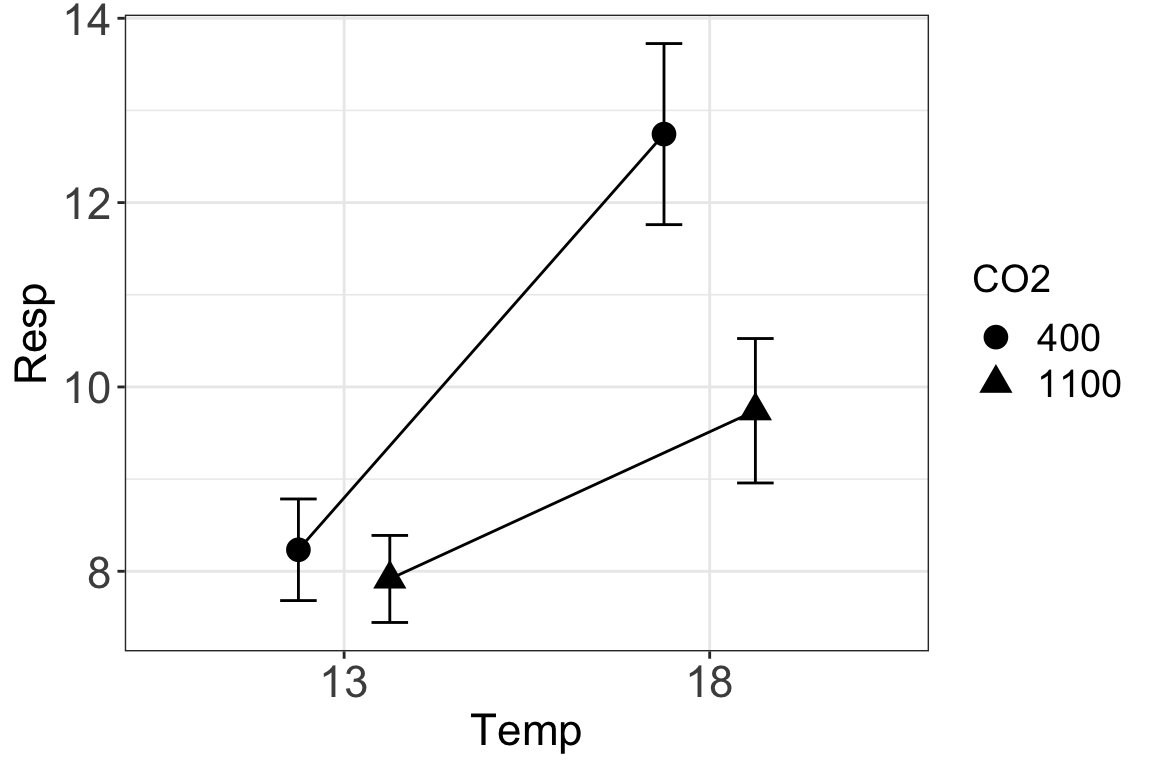
\includegraphics{Walker-elementary-statistical-modeling-draft_files/figure-latex/urchin-interaction-plot-1.pdf}

In this interaction plot, the \(X\)-axis contains the two \(Temp\)
treatment levels and the \(Y\)-axis is the outcome (\(Resp\)). The plot
shows the four cell means indicated by the circles (low CO2 levels) or
triangles (high CO2 levels). The solid lines connect the cell means
\emph{across Temp levels within CO2 levels}.

\begin{enumerate}
\def\labelenumi{\arabic{enumi}.}
\tightlist
\item
  The slope of a line is the effect of \(Temp\) on \(Resp\)
\item
  The relative \emph{elevation} of the lines is the effect of \(CO2\) on
  \(Resp\)
\item
  The difference in slope \emph{or} the relative elevation at each level
  of \(Temp\) is the interaction effect
\end{enumerate}

Let's deconstruct this. The top (CO2-) line is the effect of \(Temp\) at
the control (400 \(\mu\)ATM) value of \(CO2\). The slope of the bottom
(CO2+) line is the effect of \(Temp\) at the high (1100 \(\mu\)ATM)
value of \(CO2\). \emph{These lines have different slopes}, or the slope
\emph{is conditional on} the level of CO2. This means that the effect of
\(Temp\) on respiration is \emph{conditional on the value of \(CO2\)}.
Think about this. This is what an interaction implies--conditional
effects.

At the reference temperature (13 C), the CO2+ line is barely below the
CO2- line. But at the high temperature (18 C), the CO2+ line is far
below the CO2- line. That is, the relative elevation (the \(CO2\)
effect) is conditional on the level of \(Temp\). It will always be the
case that if the effect of Factor A is conditional on the levels of
Factor B, then the effect of Factor B will be conditional on the levels
of Factor A.

An interaction plot is an okay plot. It doesn't show the data, only a
descriptive summary (means and standard errors). If we are interested in
the interaction effect, it doesn't give us a very good sense of the
error in this effect. And \emph{that} is a problem because with real
data, two lines are never precisely parallel. Our interpretation of the
similarity of the slopes would probably mostly reflect our pre-conceived
scientific model.

\section{Recommendations}\label{recommendations-1}

\begin{enumerate}
\def\labelenumi{\arabic{enumi}.}
\tightlist
\item
  Should an interaction term be dropped from a model? In biological
  data, there will almost certainly be an interaction effect with
  everything. The goal, then, should be to model the effect and use the
  estimate and the uncertainty in the effect, \emph{in combination with
  the goals of the analysis}, to make any decision about dropping a
  term.
\end{enumerate}

\section{Working in R}\label{working-in-r-2}

A \textbf{full-factorial} model with two factors is specified in the
model formula as \texttt{y\ \textasciitilde{}\ A*B} where A is the first
factor, and B is the second factor. R expands this formula to
\texttt{y\ \textasciitilde{}\ A\ +\ B\ +\ A:B} where the colon indicates
an interaction (multiplicative) effect.

\begin{Shaded}
\begin{Highlighting}[]
\CommentTok{# re-label levels and convert to factors.}
\NormalTok{urchin1 <-}\StringTok{ }\KeywordTok{copy}\NormalTok{(urchin)}
\NormalTok{urchin1[, CO2}\OperatorTok{:}\ErrorTok{=}\KeywordTok{factor}\NormalTok{(}\KeywordTok{ifelse}\NormalTok{(CO2}\OperatorTok{==}\DecValTok{400}\NormalTok{,}\StringTok{"-"}\NormalTok{, }\StringTok{"+"}\NormalTok{))]}
\NormalTok{urchin1[, Temp}\OperatorTok{:}\ErrorTok{=}\KeywordTok{factor}\NormalTok{(}\KeywordTok{ifelse}\NormalTok{(Temp}\OperatorTok{==}\DecValTok{13}\NormalTok{, }\StringTok{"-"}\NormalTok{, }\StringTok{"+"}\NormalTok{))]}
\NormalTok{fit <-}\StringTok{ }\KeywordTok{lm}\NormalTok{(Resp }\OperatorTok{~}\StringTok{ }\NormalTok{Temp}\OperatorTok{*}\NormalTok{CO2, }\DataTypeTok{data=}\NormalTok{urchin1) }\CommentTok{# use urchin1 data with relabeled levels}
\KeywordTok{coef}\NormalTok{(}\KeywordTok{summary}\NormalTok{(fit))}
\end{Highlighting}
\end{Shaded}

\begin{verbatim}
##               Estimate Std. Error    t value     Pr(>|t|)
## (Intercept)  8.2333333  0.7255577 11.3475922 3.626935e-10
## Temp+        4.5100000  1.0260936  4.3953106 2.792573e-04
## CO2+        -0.3166667  1.0260936 -0.3086138 7.608069e-01
## Temp+:CO2+  -2.6850000  1.4511155 -1.8503007 7.910035e-02
\end{verbatim}

The first thing this script does is to re-label the levels of Temp and
CO2. The relabeling is more aesthically pleasing in the tabled output.
If we didn't relable, it would be necessary to convert CO2 and Temp to
factors or else R would treat these as numeric and not factors.

The additive model is specified by the formula
\texttt{y\ \textasciitilde{}\ A\ +\ B}

\begin{Shaded}
\begin{Highlighting}[]
\NormalTok{fit <-}\StringTok{ }\KeywordTok{lm}\NormalTok{(Resp }\OperatorTok{~}\StringTok{ }\NormalTok{Temp }\OperatorTok{+}\StringTok{ }\NormalTok{CO2, }\DataTypeTok{data=}\NormalTok{urchin1) }\CommentTok{# use urchin1 data with relabeled levels}
\KeywordTok{coef}\NormalTok{(}\KeywordTok{summary}\NormalTok{(fit))}
\end{Highlighting}
\end{Shaded}

\begin{verbatim}
##              Estimate Std. Error   t value     Pr(>|t|)
## (Intercept)  8.904583  0.6636207 13.418183 9.038657e-12
## Temp+        3.167500  0.7662831  4.133590 4.721000e-04
## CO2+        -1.659167  0.7662831 -2.165214 4.203445e-02
\end{verbatim}

\section{Problems}\label{problems-3}

\begin{enumerate}
\def\labelenumi{\arabic{enumi}.}
\item
  Draw four \(2 \times 2\) tables and label the row and column headers
  using the levels of the urchin treatment. In the first table, insert
  the cell means. In the 2nd table, insert the equation for the
  coefficient. In the third table, solve the equations. And in the
  fourth column, insert the estimates from the table above. Are tables 3
  and 4 the same? If not, you've goofed somewhere.
\item
  Frew et al. (2017) showed that increasing atomospheric CO2 increases
  grub activity in the soil which in turn increases root damage to
  sugarcane. They used a 2 x 2 experiment to then show that silicon
  added to the soild decreased the damage to the roots by the grubs
  (silicon minerals are very hard and plants uptake silicon from the
  soil to mineralize tissues to protect against insect damage). There
  are lots of analyses in the paper, but I want you to reproduce Fig.
  4b, but using gg\_interaction\_plot and fit the model using lm.
\end{enumerate}

(The treatment assignments are in a different file than the experimental
results. Use the \texttt{merge} function to glue the two tables
together, keying on the common column ``plant'')

\begin{enumerate}
\def\labelenumi{\arabic{enumi}.}
\tightlist
\item
  \textbf{file name}: ``canegrub\_feedingtrial.csv''
\item
  \textbf{file name}: ``treatments.csv''
\item
  \textbf{source}:
  \url{https://datadryad.org/resource/doi:10.5061/dryad.r3s16}
\end{enumerate}

\begin{figure}
\centering
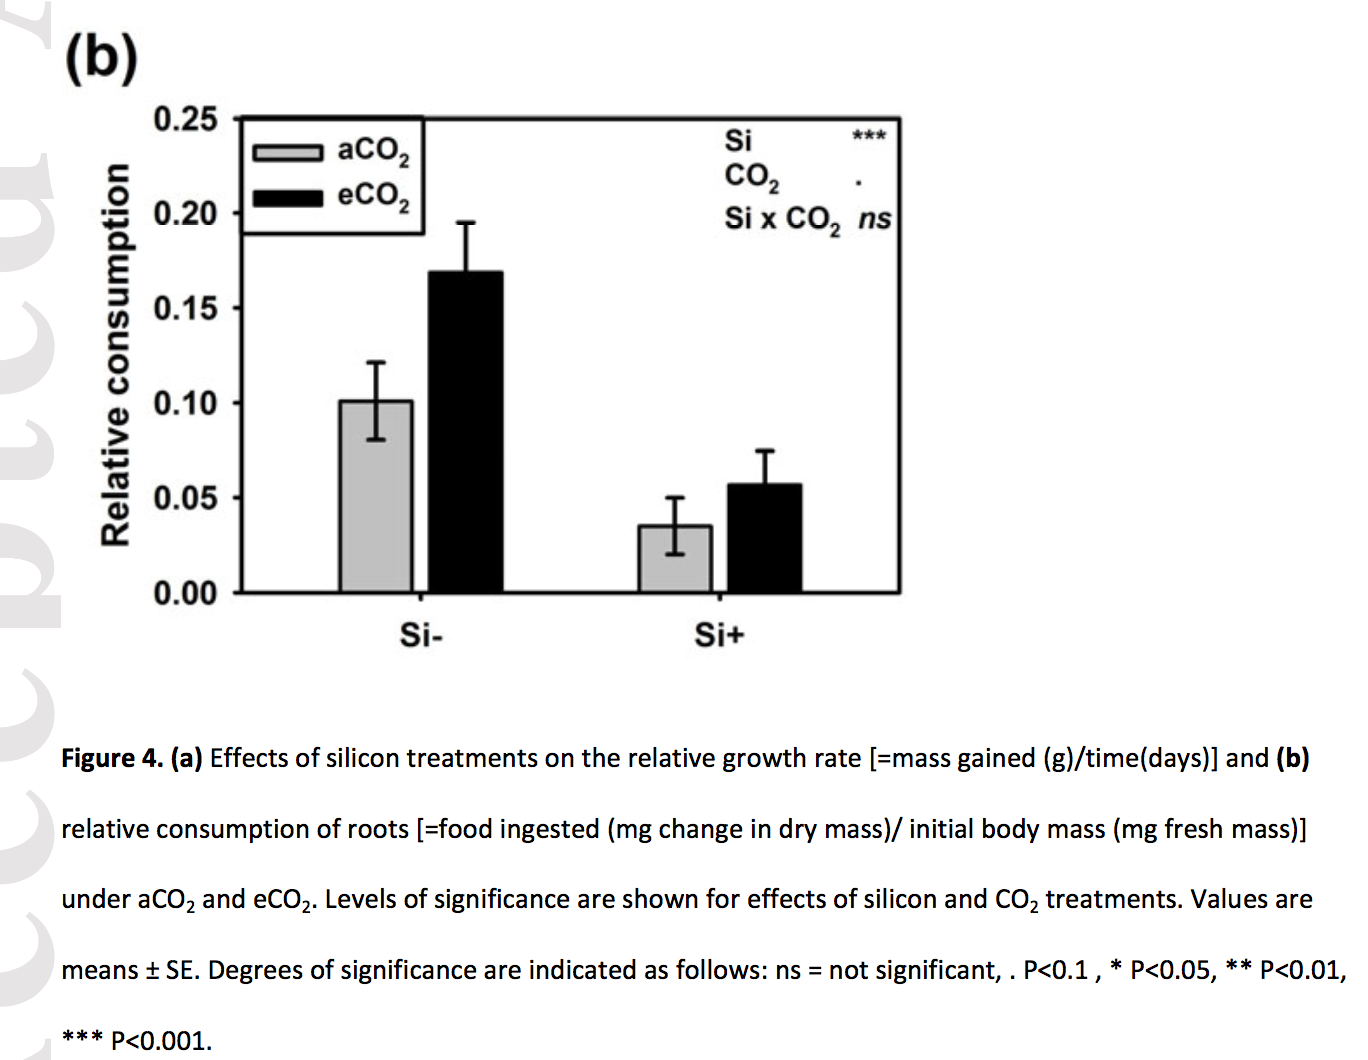
\includegraphics[width=0.50000\textwidth]{images/frew_fig_4b.png}
\caption{Frew et al. Figure 4b}
\end{figure}

\begin{enumerate}
\def\labelenumi{\arabic{enumi}.}
\setcounter{enumi}{2}
\tightlist
\item
  Kardol et al investigated the effect of moss growth in response to
  rainfall and community structure. Analyze the effect of these two
  factors on biomass gain and generate a Harrell plot alternative to
  their bar plot in Fig. 3 (see below). What is striking about your plot
  compared to theirs?
\end{enumerate}

\textbf{Filename} ``Data file for Dryad.xlsx'' \textbf{sheet} ``Data''
**Source*:**
\url{https://datadryad.org/resource/doi:10.5061/dryad.66d5f}

\begin{figure}
\centering
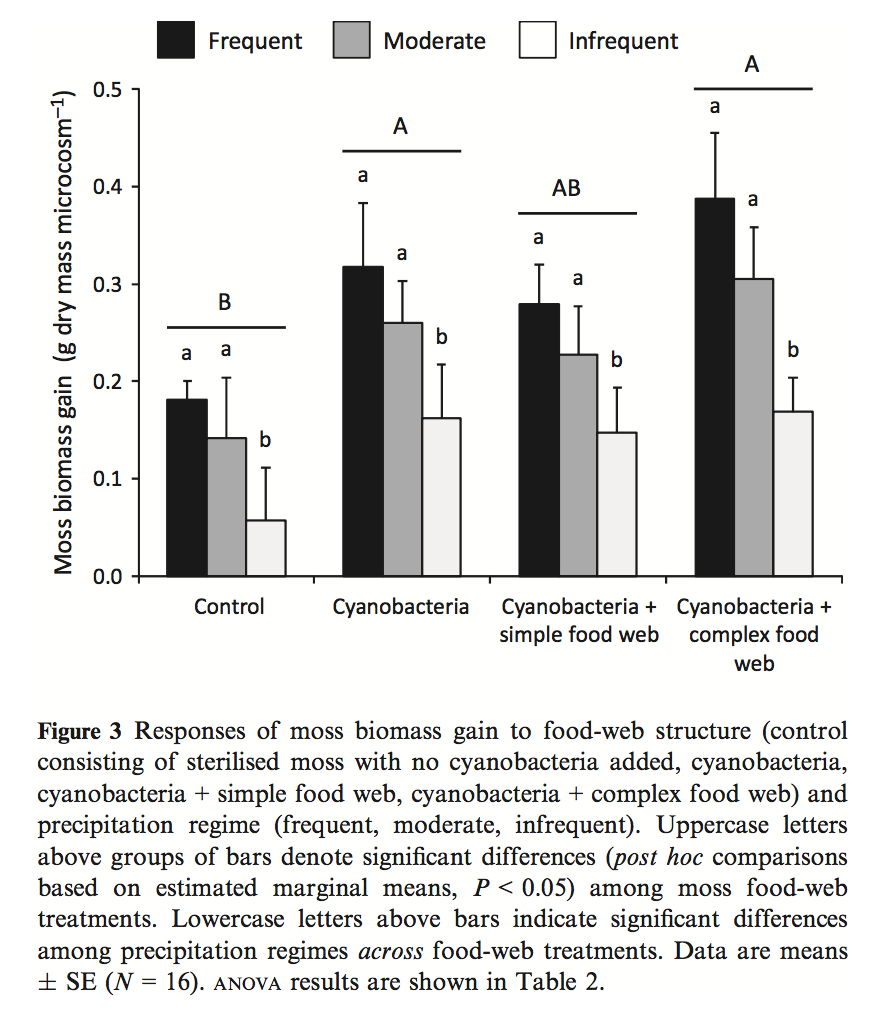
\includegraphics[width=0.50000\textwidth]{images/kardol_fig_3.png}
\caption{Kardol et al. Figure 3}
\end{figure}

\begin{enumerate}
\def\labelenumi{\arabic{enumi}.}
\setcounter{enumi}{3}
\tightlist
\item
  (Grad students only) Generate a fake experiment! The experiment should
  have two factors each with two levels. Experiment with power by
  varying sample size and effect size.
\end{enumerate}

\chapter{ANOVA}\label{anova}

Treatment effects are most often analyzed using ANOVA, which is short
for ``Analysis of Variance''. This is somewhat of an odd name for a
method to test for treatments effects - what do differences in means
have to do with an analyis of variance? The name makes sense in light of
the decomposition of the total variance into a model variance and the
residual variance (chapter xxx). If there are differences among the
means, then the total variance is increased because of variation among
groups.

The engine underneath ANOVA is a linear model. If the model has a single
categorical factor, the ANOVA is \textbf{one-way}. If the model has two
categorical factors it is a two-way ANOVA. If the model has a single
categorical factor and one continuous factor it is an ANCOVA, short for
\textbf{analysis of covariance} (next chapter). More complex
experimental designs classically analyzed with ANOVA are nested,
split-plot, latin-square, and many others.

\section{Summary of usage}\label{summary-of-usage}

If you choose to report an ANOVA, also report the effects and their
uncertainty in some way, either the model coefficients or contrasts.

\begin{enumerate}
\def\labelenumi{\arabic{enumi}.}
\tightlist
\item
  ANOVA generates a table with one row for each term in the linear
  model. A term is a factor or a covariate or an interaction. For a
  two-way factorial ANOVA, these terms are the two main effects and the
  interaction effect.
\item
  The ANOVA generates an \(F\) and \(p\)-value for the whole model and
  for each term in the ANOVA table.
\item
  The \(p\)-value of an interaction term is often used as a decision
  rule to interpret the main effects. If \(p \le 0.05\) then do not
  interpret the main effects but instead examine the condition
  (``simple'') effects. If \(p > 0.05\), then interpret the main
  effects. Regardless, this sort of decision rule is itself
  controversial, and for good reason.
\item
  If the main effects are to be interpreted, some statisticians advocate
  re-fitting the model without the interaction effect, others advocate
  interpreting the main effects with the interaction term in the model.
  This only matters if the design is unbalanced (see below).
\item
  Regardles of any decision, always plot the data using a Harrell plot
  or interaction plot to understand and communicate the magnitude and
  pattern of interaction.
\item
  For factors with more than two levels, the \(p\)-value is often used
  as a decision rule to dissect the factor with post-hoc tests, such as
  Tukey HSD.
\item
  A design is balanced if all the cells have the same number of
  replicates. A design is unbalanced if one or more of the cells has a
  different number of replicates. Unbalanced designs make it necessary
  to make decisions, none of which are perfect, and all of which are
  controversial. Some statisticians have even advocated randomly
  excluding data until the design is back in balance. Don't do this.
\item
  There are multiple ways to decompose the sum of squares. I highlight
  the major three: Type I (sequential), Type II (partial sequential),
  and Type III. Most statistics software and introductory statistics
  books default to Type III and, consequently, many researchers are
  unaware that Types I and II exist. R's default is Type I, and this can
  make a difference if the design is unbalanced. This is \emph{not} a
  rare error in publications.
\item
  Because R defaults to Type I sum of squares, the \(p\)-value of a
  factor depends on the order of the factors in the model if the design
  is unbalanced. This is a feature, not a bug.
\item
  ANOVA based on type II sum of squares do not depend on factor order if
  the design is unbalanced, but it does assume that the interaction is
  zero.
\item
  ANOVA based on type III sum of squares do not depend on order if the
  design is unbalanced and does not assume the interaction is zero.
\item
  If the design is balanced, Type I, II, and III sum of squares generate
  the same ANOVA table. And the ANOVA table of just the main effects is
  the same as the ANOVA table that includes the interaction term. None
  of this is true when the design is unbalanced, However, the decision
  to use type II or type III is very controversial.
\end{enumerate}

\section{Example: a one-way ANOVA using the vole
data}\label{example-a-one-way-anova-using-the-vole-data}

The vole data has a single factor (``treatment'') with three levels
(``control'', ``vitamin\_E'', ``vitamin\_C''). In statistics textbooks
that emphasize hypothesis testing, the ``Which test should I use''
flowchart would guide a researcher given this design to a single
classification, or one-way ANOVA, since a t-test can only compare two
levels but an ANOVA can compare more than two levels. There are better
ways to think about what ANOVA is doing, but okay.

Here is an ANOVA table of the vole data:

\begin{tabular}{l|r|r|r|r|r}
\hline
  & Df & Sum Sq & Mean Sq & F value & Pr(>F)\\
\hline
treatment & 2 & 248446 & 124223.0 & 2.95 & 0.057\\
\hline
Residuals & 93 & 3912751 & 42072.6 &  & \\
\hline
\end{tabular}

I'll explain all the parts of the ANOVA table later, but for now, focus
on the \(p\)-value, which is that most researchers want out of the
table. What null hypothesis does this \(p\)-value test? The p-value
gives the probability of the observed \(F\) or larger \(F\), if the null
were true. The null hypothesis models the data as if they were sampled
from a single, normal distribution and randomly assigned to different
groups. Thus the null hypotheis includes the equality of the means among
factor levels. In the vole data, the single treatment factor has three
levels and a small \(p\)-value could occur because of a difference in
means between the vitamin\_E treatment and control, or between the
vitamin\_C treatment and control, or between the two vitamin treatments.
The \(p\)-value or ANOVA table doesn't indicate what is different, only
that the observed \(F\) is unexpectedly large if the null were true. As
a consequence, researchers typically interpret a low \(p\)-value in an
ANOVA table as evidence of ``an effect'' of the term but have to use
additional tools to dissect this effect. The typical additional tools
are either \textbf{planned comparisons}, which are contrasts among a
subset of a priori identified treatment levels (or groups of levels) or
unplanned comparisons (``post-hoc'' tests) among all pairs of levels.

The \(p\)-value in the ANOVA table acts as a decision rule: if
\(p < 0.05\) then it is okay to further dissect the factor with planned
comparisons or post-hoc tests because the significant \(p\) ``protects''
the type I error of further comparisons. I'm not fond of using
\(p\)-values for these sorts of decision rules.

\section{Example: a two-way ANOVA using the urchin
data}\label{example-a-two-way-anova-using-the-urchin-data}

Let's use the urchin data from the previous chapter xxx to explore the
ANOVA table, which is what is typically reported. The experiment has two
factors (\(Temp\) and \(CO2\)), each with two levels. Here is the linear
model

\begin{equation}
Resp = \beta_0 + \beta_1 Temp + \beta_2 CO2 + \beta_3 TempCO2 + \varepsilon
\end{equation}

In order to understand factorial ANOVA (or any ANOVA with multiple
factors), it is useful to know the difference between
\textbf{conditional means} and \textbf{marginal means}

\begin{verbatim}
##          CO2-  CO2+ Temp-mm
## Temp-   8.233 7.917   8.075
## Temp+  12.743 9.742  11.243
## CO2-mm 10.488 8.829   9.659
\end{verbatim}

In the table above, the upper, left \(2 \times 2\) grid of cells are the
conditional means, which are the means of each group, where a group is a
specific combination of factor levels. The first two values of the third
row are the marginal means for CO2. The first (10.488) is the mean of
the two means when CO2=CO2-. This can be written as
\(\mathrm{E}(Resp|CO2-)\). The second (8.829) is the mean of the two
means when CO2=CO2+, or \(\mathrm{E}(Resp|CO2+)\). The first two
elements of the third column are the marginal means for Temp. These are
\(\mathrm{E}(Resp|Temp-)\) and \(\mathrm{E}(Resp|Temp+)\). The bottom
right value (9.659) is the grand mean.

A \textbf{conditional effect} is a difference between conditional means.
For example the conditional effect of \(Temp\) \emph{conditional on}
CO2=CO2- is \(12.743-8.233\). A \textbf{marginal effect} is a difference
in marginal means within a factor, for example the marginal effect of
\(Temp\) is \(11.243 - 8.075\).

Here is the ANOVA table of the urchin data

\begin{tabular}{l|r|r|r|r|r}
\hline
  & Df & Sum Sq & Mean Sq & F value & Pr(>F)\\
\hline
Temp & 1 & 60.2 & 60.2 & 19.1 & 0.0003\\
\hline
CO2 & 1 & 16.5 & 16.5 & 5.2 & 0.0332\\
\hline
Temp:CO2 & 1 & 10.8 & 10.8 & 3.4 & 0.0791\\
\hline
Residuals & 20 & 63.2 & 3.2 &  & \\
\hline
\end{tabular}

This ANOVA table uses what are called Type 3 sum of squares, which is
\emph{NOT} the default in R but is the default in many other statistics
software and is, therefore, the \emph{only} type of ANOVA that many
researchers know (and, many researchers are unaware that there are
multiple types of ANOVA table). Understanding these differences is
important, at least if one is reporting ANOVA tables. I'll return to the
importance of this later.

\subsection{How to read an ANOVA
table}\label{how-to-read-an-anova-table}

An ANOVA table has a row for each term in the underlying linear model --
each of these adds a component of variance to the total, and a row for
the residual variance (this residual variance row is frequently excluded
from the published table). The urchin model has three terms (one level
of \(Temp\), one level of \(CO2\), and one interaction). The statistics
for each term are

\begin{enumerate}
\def\labelenumi{\arabic{enumi}.}
\tightlist
\item
  \textbf{Degrees of Freedom} (df) -- If the term is a factor, the df
  will equal the number of levels (\(k\)) for the factor minus 1. Think
  of it this way: the contribution of the variance due to a factor is a
  function of the variability of the \(k\) level means around the grand
  mean. How many degrees of independent variation do these level means
  have, given that we know the grand mean? The answer is \(k-1\) -- once
  the values of \(k-1\) level means are written down, the \(k\)th level
  mean has no freedom to vary; its value has to be
  \(k\bar{\bar{Y}} - \sum_i^{k-1}{Y_i}\). For an interaction term, the
  df is the product of the df of each of the factors in the interaction.
\item
  \textbf{Sum of Squares} -- the sum of squared differences between the
  modeled value and the grand mean. In addition to a sum of squares for
  each term, a \textbf{residual mean square} is computed as the sum of
  squared differences between the measured and modeled values.
\item
  \textbf{Mean Square} -- The sum of squares divided by the df (this is
  a ``mean'' with df acting as the number of things that were summed).
\item
  \textbf{F-ratio} -- the Mean Square of the term dived by the residual
  mean square.
\item
  \textbf{p-value} -- the p-value for the F-ratio. F is compared to an
  F-distribution, which is a distribution of F-ratios under the null.
\end{enumerate}

\subsubsection{Each row in the table tests a null
hypothesis}\label{each-row-in-the-table-tests-a-null-hypothesis}

The row for each term in an ANOVA table tests a null hypothesis. In
order to understand the null hypotheses, I need to define a few more
terms

For the ANOVA table above, which uses Type 3 sum of squares, the
probabilities are

\begin{enumerate}
\def\labelenumi{\arabic{enumi}.}
\tightlist
\item
  Temp -- \(p = \mathrm{prob}(F \ge F_o|CO2, Temp:CO2)\). The null is no
  difference in means conditional on the level of CO2 and Temp:CO2. This
  is equivalent to no difference between the grand mean and the marginal
  mean of Temp+, or
\end{enumerate}

\begin{equation}
b_1 = \overline{\overline{Resp}} - \mathrm{E}(Resp|Temp^+)
\end{equation}

\begin{enumerate}
\def\labelenumi{\arabic{enumi}.}
\setcounter{enumi}{1}
\tightlist
\item
  CO2-- \(p = \mathrm{prob}(F \ge F_o|Temp, Temp:CO2)\). The null is no
  difference in means conditional on the level of Temp and Temp:CO2.
  This is equivalent to no difference between the grand mean and the
  marginal mean of CO2+, or
\end{enumerate}

\begin{equation}
b_2 = \overline{\overline{Resp}} - \mathrm{E}(Resp|CO2^+)
\end{equation}

\begin{enumerate}
\def\labelenumi{\arabic{enumi}.}
\setcounter{enumi}{2}
\tightlist
\item
  Temp:CO2 -- \(p = \mathrm{prob}(F \ge F_o|Temp, CO2)\). The null is no
  difference in means conditional on the level of Temp and CO2. This is
  equivalent to the difference between the conditional mean of
  Temp+/CO2+ and the expected conditional mean of Temp+/CO2+ if there
  were no interaction.
\end{enumerate}

\begin{equation}
b_3 = \mathrm{E}(Resp|Temp^+, CO2^+) - (\overline{\overline{Resp}} - b_1 - b_2)
\end{equation}

As noted in the equations, these three differences are the coefficients
of the linear model behind the ANOVA. Here is the coefficient table

\begin{tabular}{l|r|r|r|r}
\hline
  & Estimate & Std. Error & t value & Pr(>|t|)\\
\hline
(Intercept) & 9.66 & 0.36 & 26.6 & 0.00000\\
\hline
Temp1 & -1.58 & 0.36 & -4.4 & 0.00030\\
\hline
CO21 & 0.83 & 0.36 & 2.3 & 0.03325\\
\hline
Temp1:CO21 & -0.67 & 0.36 & -1.9 & 0.07910\\
\hline
\end{tabular}

In ANOVA with type 3 sum of squares, the dummy variables are coded using
effect coding, which differs from the dummy coding introduced in chapter
xxx. The consequence is that the \textbf{grand mean} (the mean of
\(Resp\) across all values) is now the ``reference'' value. The
intercept in this table, then, is the grand mean. The coefficients are
\emph{differences from the grand mean}, as described above.

Use the table of conditional and marginal effects above to check that
the coefficients equal the differences in the equations above. Also not
that the \(p\)-values for the effects in the coefficient table equals
the \(p\)-values in the ANOVA table.

It is important to note that this table differs from the coefficient
table with dummy coding because that reference is the mean of Temp-/CO2-
and not the grand mean.

\begin{tabular}{l|r|r|r|r}
\hline
  & Estimate & Std. Error & t value & Pr(>|t|)\\
\hline
(Intercept) & 8.23 & 0.73 & 11.3 & 0.00000\\
\hline
TempTemp+ & 4.51 & 1.03 & 4.4 & 0.00028\\
\hline
CO2CO2+ & -0.32 & 1.03 & -0.3 & 0.76081\\
\hline
TempTemp+:CO2CO2+ & -2.68 & 1.45 & -1.9 & 0.07910\\
\hline
\end{tabular}

Importantly, note that \(p\)-values for \(b_1\) (the Temp effect) and
\(b_2\) differ between the two tables. This is because the \(t\)-value
tests different hypotheses! In the coefficient table with effect coding
(that behind the ANOVA with type 3 sums of squares), the \(p\)-value
tests marginal effects and so is a function of both marginal means
within a factor. By contrast, in the coefficient table with dummy
coding, the \(p\)-value tests conditional effects, and so is only a
function of the conditional means when the other factor is at its
reference level (right? The coefficient \(b_1\) in the dummy coded
coefficient table is the effect of only increasing \(Temp\) -- \(CO2\)
is left at its reference level). For the interaction effect, the
coefficient differs between the effects coded model and the dummy coded
model (because different reference means) but the \(p\)-value ultimately
tests the same hypothesis (non-additive effects of the factors) and so
the \(t\) and \(p\) values are the same.

\subsubsection{What to do after ANOVA?}\label{what-to-do-after-anova}

Researchers frequently report ANOVA statistics (\(F\) and \(p\) values)
for factorial models in a way that suggests that they misunderstand the
hypotheses tested. It probably doesn't help that there is a
long-standing debate among statisticians about the most sensible
strategy for interpreting factorial ANOVA results. And it doesn't help
that the default ANOVA table in R can suggest a very different
interpretation than the default ANOVA table in some other software
packages.

Here are three strategies for interpreting a factorial ANOVA table that
uses Type III sum of squares. All strategies use \(p\)-values to make a
series of decision rules. In the first strategy, which is a type of
model simplification or model selection, a researcher starts with the
interactions at the bottom of the ANOVA table and works up, eliminating
terms with \(p > 0.05\) and re-fitting the reduced model before
interpreting main effects. In the second strategy, the researcher uses
the original ANOVA table that includes all terms to interpret main
effects.

\textbf{Strategy 1}

\begin{enumerate}
\def\labelenumi{\arabic{enumi}.}
\tightlist
\item
  is interaction \emph{p} \textless{} 0.05?

  \begin{enumerate}
  \def\labelenumii{\alph{enumii}.}
  \tightlist
  \item
    if yes, then do NOT test main effects. Show a graph to show pattern
    of conditional effects. Test conditional effects if this is of
    interest.
  \item
    if no, then refit model without the interaction and test main
    effects -- This now is equivalent to ANOVA using Type II sum of
    squares.

    \begin{enumerate}
    \def\labelenumiii{\arabic{enumiii}.}
    \setcounter{enumiii}{1}
    \tightlist
    \item
      is main effect \emph{p} \textless{} 0.05\$?

      \begin{enumerate}
      \def\labelenumiv{\alph{enumiv}.}
      \tightlist
      \item
        if yes, then keep in model
      \item
        if no, then refit model without that main effect
      \end{enumerate}
    \end{enumerate}
  \end{enumerate}
\end{enumerate}

\textbf{Strategy 2}

\begin{enumerate}
\def\labelenumi{\arabic{enumi}.}
\setcounter{enumi}{1}
\tightlist
\item
  is interaction \emph{p} \textless{} 0.05?

  \begin{enumerate}
  \def\labelenumii{\alph{enumii}.}
  \tightlist
  \item
    if yes, then do NOT test main effects. Show a graph to show pattern
    of conditional effects. Test conditional effects if this is of
    interest.
  \item
    if no, then use the same table as the test of the main effects. This
    is interpreting the main effects with the interaction term in the
    model. This is the logic of ANOVA using type III sum of squares.
  \end{enumerate}
\end{enumerate}

\textbf{Strategy 3}

\begin{enumerate}
\def\labelenumi{\arabic{enumi}.}
\setcounter{enumi}{2}
\tightlist
\item
  is interaction \emph{p} \textless{} 0.05?

  \begin{enumerate}
  \def\labelenumii{\alph{enumii}.}
  \tightlist
  \item
    if yes, then look at interaction plot to determine if it makes sense
    test main effects. For example, if CO2+ had obviously lower \(Resp\)
    at both levels of \(Temp\), even if one was much lower (ie.
    interactaction), then some people would say that the test of the
    main effect is meaningful. Test conditional effects if this is of
    interest.
  \item
    if no, then use the same table as the test of the main effects
  \end{enumerate}
\end{enumerate}

In general, statisticians advise against strategy 3 (interpreting main
effects in the presence of interaction) -- its not wrong, its just that
a main effect has an awkward interpretation if there is an interaction.
Of course this is true if there is \emph{any} interaction term in the
model, not just a statistically significant term. The controversy is
more, if the interaction \(p\) is not significant, then do we implement
stategy 1 (refit model excluding interaction to test main effects) or
strategy 2 (use full factorial anova table to test main effects).

\begin{tabular}{l|r|r|r|r|r}
\hline
  & Df & Sum Sq & Mean Sq & F value & Pr(>F)\\
\hline
Temp & 1 & 45.2 & 45.2 & 14.5 & 0.0011\\
\hline
CO2 & 1 & 4.1 & 4.1 & 1.3 & 0.2630\\
\hline
Temp:CO2 & 1 & 14.8 & 14.8 & 4.8 & 0.0413\\
\hline
\end{tabular}

then one shouldn't report the ANOVA results using something like
``Temperature had a significant effect on metabolism
(\(F_{1,20} = 14.5\), \(p=0.001\)). There was no effect of CO2 on
metabolism (\(F_{1,20} = 4.1\), \(p=0.26\))''. There was a significant
interaction effect between Temperature and CO2 on metabolism
(\(F_{1,20} = 14.8\), \(p=0.04\))``. If one accepts that the small
interaction \(p\)-value is evidence of an interaction effect then this
interpretation of the main factors makes no sense, as the first two
results imply that the interaction effect is zero (or, that there is a
constant effect of \(Temp\) or \(CO2\) across both levels of the other
factor), which is then contradicted by the third result.

More specifically, if one is using a \(p\)-value to guide decision
making, then a significant interaction \(p\) indicates that there is no
single ``main'' effect of a factor. Instead, the effect of \(Temp\) is
conditional on the level of \(CO2\), and the effect of \(CO2\) is
conditional on the level of \(Temp\). This is easily seen in the
interaction plot, where the effect of \(Temp\) is large when \(CO2\) is
high but much smaller when \(CO2\) is low. Indeed, the effect of
\(Temp\) at the low CO2 is 0.16.

Instead of interpreting the factors as constant effects, A better
strategy is to compare the \textbf{conditional effects}, that is, the
effects of \(Temp\) within each level of \(CO2\) and the effects of
\(CO2\) within each level of \(Temp\) (conditional effects are sometimes
called the ``simple effects'').

The controversy arises in what to do after an ANOVA if the interaction
effect has a non-significant \(p\)-value. At this point, I am punting
instead of explaining the basis for the controversy, because ultimately
I think the major problem with both strategies is the use of null
hypothesis significance testing to make analysis decisions.

In fact, the entire reason that I use the urchin data as the example for
factorial ANOVA is because it beautifully illustrates the absurdity of
the interaction \(p\)-value decision rule. Why should we interpret the
results of the ANOVA when the interaction \(p\) is 0.079 differently
than when the interaction \(p\) is 0.04? Remember, the \(p\)-value is a
``sample'' statistic (in the sense that it is entirely a function of the
sampled data) and in conditions of low power (which is likely, but not
necessarily, true for the urchin data given n=6), a \(p\)-value is
highly variable.

There are several problems with this approach. 1) a \(p\)-value is not
evidence of ``no effect'', 2) the power to test interaction effects is
small relative to that for the main effects (this is a general rule, not
something specific to these data), 3) the interaction SS accounts for
about 7.2\(\%\) of the total SS, which doesn't seem inconsequential, and
4) the interaction \(p\)-value is small enough to raise a red flag, and,
most importantly, 5) the confidence interval of the interaction effect
indicates that the large, negative values of the interaction are
\emph{as consistent with the data} as trivially small values (or a value
of zero). But the CI is not in an ANOVA table and many researchers fail
to report it. These five points suggest that this experiment be
replicated, with a larger sample size, to get a better estimate of the
interaction effect. The problem of course is that experiments are rarely
replicated, except in biomedical research.

The absurdity of the \(p\)-value decision rule strategy for
interpretation of effects after an ANOVA is highlighted by comparing the
forest plot of model coefficients of the real and fake urchin data. It
would be absurd to use an ANOVA table to interpret these patterns as
radically different (one without an interaction and constant main
effects, the other with an interactioni and conditional effects).

\begin{figure}
\centering
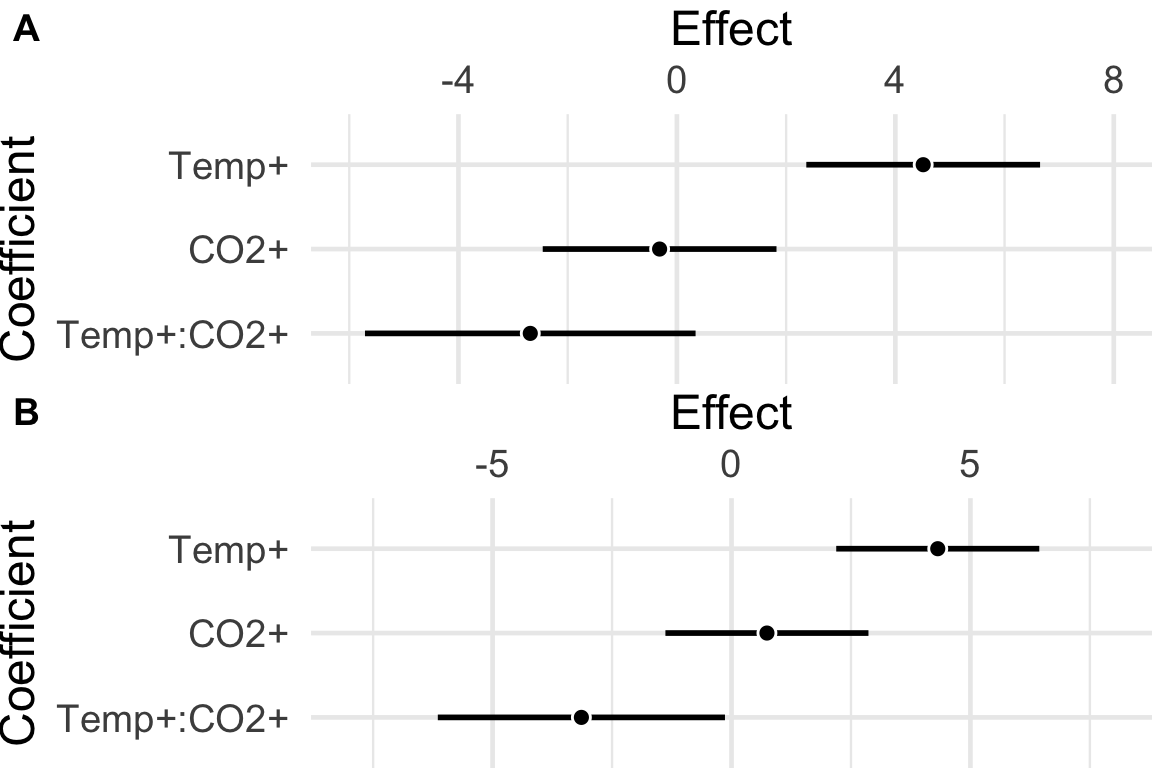
\includegraphics{Walker-elementary-statistical-modeling-draft_files/figure-latex/urchin-anova-ggplot-1.pdf}
\caption{\label{fig:urchin-anova-ggplot}Forest plots (the upper part of a
Harrell plot) of the actual and fake urchin data. A) Real urchin data.
The interaction effect is not significant (\(p=0.079\)). B) Fake urchin
data. The interaction effect is significant (\(p=0.04\)).}
\end{figure}

\subsection{Better practice -- estimates and their
uncertainty}\label{better-practice-estimates-and-their-uncertainty}

As emphasized in the previous chapter, the decision to include or
exclude an interaction effect in the model should not be based on a
\(p\)-value but on the goals of the model.

\begin{enumerate}
\def\labelenumi{\arabic{enumi}.}
\item
  If the goal is the interaction (because a scientific model predicts
  one, or because this is biology and everything is conditional), then
  estimate the interaction effect (as a coefficient of the model!) and
  its uncertainty, including a CI and \(p\)-value. There is no
  controversy on how to estimate this effect and its uncertainty. The
  coefficient will be different between dummy and effect coded models
  but this is okay because they have different specific interpretations
  but the same general interpretation. Use a Harrel plot with the
  coefficients (including the interaction coefficient) to show this
  estimate and uncertainty.
\item
  If the goal is to estimate constant main effects, then exclude the
  interaction effect from the model and report the main effects (again,
  as coefficients from the model or contrasts if other pairwise effects
  are desired) with their uncertainty. Use an interaction plot (or
  bottom part of the harrell plot) to justify forcing the interaction to
  zero (for example the interaction effect adds little to the total sum
  of squares or the interpretation of a single main effect or two (or
  more) conditional effects would be the same. Use a Harrel plot that
  excludes the interaction term to show these main effects and
  uncertainty.
\item
  And if a researcher is interested in the effects of the factors but
  there is strong evidence for a non-trivial interaction, then report
  the conditional effects (as contrasts) with their uncertainty. Use a
  Harrel plot that includes the interaction term to show these
  conditional effects and uncertainty. If there is an obvious
  interaction, it probably doesn't make sense to interpret the main
  effects, contrary to what some people argue. If there is a positive
  effect of factor A across all levels of factor B, we don't really need
  a \(p\)-value to test that the average of these positive effects is
  significant. This doesn't add value to the plot and any conditional
  effects that are reported.
\end{enumerate}

Notice that an ANOVA table has no role in this recommendation.

\section{Unbalanced designs}\label{unbalanced-designs}

My recommendation above is to not bother with ANOVA, but to simply
compute the contrasts of interest using the linear model. But if you
really want to use ANOVA, you should be aware that \textbf{if the design
is unbalanced, factor order matters in the default R anova function} and
that I routinely find published ANOVA tables that report statistics
(\(F\) and \(p\) values) that are not what the authors think they are.

An \textbf{unbalanced} design is one in which the number of replicates
differs among the cell. The urchin data is balanced because there are
six replicates in each cell. If the respirometer broke before taking the
respiratory measures of the final tank, the design would be unbalanced,
one of the cells would have only five replicates.

Let's look at the effect of row order on the statistics of the urchin
data using R's default anova function.

\begin{tabular}{l|r|r|r|r|r}
\hline
  & Df & Sum Sq & Mean Sq & F value & Pr(>F)\\
\hline
Temp & 1 & 60.20 & 60.20 & 19.06 & 0.00030\\
\hline
CO2 & 1 & 16.52 & 16.52 & 5.23 & 0.03325\\
\hline
Temp:CO2 & 1 & 10.81 & 10.81 & 3.42 & 0.07910\\
\hline
\end{tabular}

\begin{tabular}{l|r|r|r|r|r}
\hline
  & Df & Sum Sq & Mean Sq & F value & Pr(>F)\\
\hline
CO2 & 1 & 16.52 & 16.52 & 5.23 & 0.03325\\
\hline
Temp & 1 & 60.20 & 60.20 & 19.06 & 0.00030\\
\hline
CO2:Temp & 1 & 10.81 & 10.81 & 3.42 & 0.07910\\
\hline
\end{tabular}

Now let's unbalance the data, by removing three random replicates (these
may be both in one cell or spread across cells. First, here is the
number of replicates in each cell:

\begin{verbatim}
##        
##         CO2- CO2+
##   Temp-    6    4
##   Temp+    6    5
\end{verbatim}

And here are the two tables with the order of Temp and CO2 reversed in
the model

\begin{tabular}{l|r|r|r|r|r}
\hline
  & Df & Sum Sq & Mean Sq & F value & Pr(>F)\\
\hline
Temp & 1 & 62.25 & 62.25 & 18.44 & 0.00049\\
\hline
CO2 & 1 & 21.49 & 21.49 & 6.36 & 0.02190\\
\hline
Temp:CO2 & 1 & 6.38 & 6.38 & 1.89 & 0.18720\\
\hline
\end{tabular}

\begin{tabular}{l|r|r|r|r|r}
\hline
  & Df & Sum Sq & Mean Sq & F value & Pr(>F)\\
\hline
CO2 & 1 & 17.59 & 17.59 & 5.21 & 0.03561\\
\hline
Temp & 1 & 66.14 & 66.14 & 19.59 & 0.00037\\
\hline
CO2:Temp & 1 & 6.38 & 6.38 & 1.89 & 0.18720\\
\hline
\end{tabular}

Several observations are important.

\begin{enumerate}
\def\labelenumi{\arabic{enumi}.}
\tightlist
\item
  the statistics for the last row, which is the interaction, does not
  change.
\item
  if these data were analyzed in the software package JMP, or SAS, or
  SSPS then \textbf{order wouldn't matter}. Here is what the tables
  would look like
\end{enumerate}

\begin{tabular}{l|r|r|r|r}
\hline
  & Sum Sq & Df & F value & Pr(>F)\\
\hline
Temp & 58.77 & 1 & 17.41 & 0.00064\\
\hline
CO2 & 19.93 & 1 & 5.90 & 0.02648\\
\hline
Temp:CO2 & 6.38 & 1 & 1.89 & 0.18720\\
\hline
\end{tabular}

\begin{tabular}{l|r|r|r|r}
\hline
  & Sum Sq & Df & F value & Pr(>F)\\
\hline
CO2 & 19.93 & 1 & 5.90 & 0.02648\\
\hline
Temp & 58.77 & 1 & 17.41 & 0.00064\\
\hline
CO2:Temp & 6.38 & 1 & 1.89 & 0.18720\\
\hline
\end{tabular}

\begin{enumerate}
\def\labelenumi{\arabic{enumi}.}
\setcounter{enumi}{2}
\tightlist
\item
  Order does not change the statistics in the coefficient table, even
  for unbalanced data:
\end{enumerate}

\begin{tabular}{l|r|r|r|r}
\hline
  & Estimate & Std. Error & t value & Pr(>|t|)\\
\hline
(Intercept) & 9.50 & 0.407 & 23.367 & 0.0000\\
\hline
Temp1 & -1.70 & 0.407 & -4.172 & 0.0006\\
\hline
CO21 & 0.99 & 0.407 & 2.430 & 0.0265\\
\hline
Temp1:CO21 & -0.56 & 0.407 & -1.374 & 0.1872\\
\hline
\end{tabular}

\begin{tabular}{l|r|r|r|r}
\hline
  & Estimate & Std. Error & t value & Pr(>|t|)\\
\hline
(Intercept) & 9.50 & 0.407 & 23.367 & 0.0000\\
\hline
CO21 & 0.99 & 0.407 & 2.430 & 0.0265\\
\hline
Temp1 & -1.70 & 0.407 & -4.172 & 0.0006\\
\hline
CO21:Temp1 & -0.56 & 0.407 & -1.374 & 0.1872\\
\hline
\end{tabular}

\subsection{What is going on in unbalanced ANOVA? -- Type I, II, III sum
of
squares}\label{what-is-going-on-in-unbalanced-anova-type-i-ii-iii-sum-of-squares}

\textbf{Type I sum of squares}. Here is the (default) ANOVA table using
Type I sum of squares for the urchin data with the three missing rows.

\begin{tabular}{l|r|r|r|r|r}
\hline
  & Df & Sum Sq & Mean Sq & F value & Pr(>F)\\
\hline
Temp & 1 & 62.248 & 62.248 & 18.4 & 0.0005\\
\hline
CO2 & 1 & 21.488 & 21.488 & 6.4 & 0.0219\\
\hline
Temp:CO2 & 1 & 6.377 & 6.377 & 1.9 & 0.1872\\
\hline
Residuals & 17 & 57.399 & 3.376 &  & \\
\hline
\end{tabular}

The default coding of dummy variables in R's \texttt{lm} function is
dummy coding, which is the coding used for Type I or \textbf{Sequential
Sum of Squares}. The hypothesis tested by each row in the ANOVA table
using Type I sum of squares is the effect of that row's term conditional
on all terms before it in the model (or above it in the table) and
ignoring all terms after it in the model (or below it in the table).

\begin{enumerate}
\def\labelenumi{\arabic{enumi}.}
\item
  The hypothesis tested by the \(p\)-value for \(Temp\) is the same as
  if \(Temp\) were the only term in the model (other than the
  intercept). That is, the means are estimated for each level of
  \(Temp\) ignoring the fact that half the replicates within each level
  of \(Temp\) experienced low \(CO2\) and half experienced high \(CO2\)
\item
  The hypothesis tested by the \(p\)-value for \(CO2\) is conditional on
  \(Temp\). That is, the difference in metabolism between \(CO2+\) and
  \(CO2-\) when \(Temp\) is ``held constant'' (or for all cases where
  \(Temp\) takes the same value). This is equivalent to the hypothesis
  that the difference in the marginal means of CO2 is zero.
\item
  The hypothesis tested by the \(p\)-value for the interaction is
  conditional on all other terms and nothing is ignored.
\end{enumerate}

\textbf{Type II sum of squares}. Here is the ANOVA table using Type II
sum of squares for the urchin data with missing values. The interaction
term is excluded from the linear model, because type II sum of squares
are used to estimate main effects ignoring the interaction (so this
would make sense only if a plot of the effects suggested a small
interaction relative to the main effects). The sum of squares for the
main effects would be the same if the interaction were included but the
residual df, and thus the F and P-values would differ.

\begin{tabular}{l|r|r|r|r|r}
\hline
  & Df & Sum Sq & Mean Sq & F value & Pr(>F)\\
\hline
Temp & 1 & 66.145 & 66.145 & 18.7 & 0.0004\\
\hline
CO2 & 1 & 21.488 & 21.488 & 6.1 & 0.0241\\
\hline
Residuals & 18 & 63.776 & 3.543 &  & \\
\hline
\end{tabular}

The hypothesis tested by each row in the ANOVA table using Type II sum
of squares is the effect of that row's term conditional on all terms
\emph{at the same level or below} but ignoring all terms at a higher
level in the model (or below it in the table). For example, the
hypothesis test for a factor is conditioned on other factors but ignores
interaction terms among the factors. Consequently, these hypotheses
tested are

\begin{enumerate}
\def\labelenumi{\arabic{enumi}.}
\item
  The hypothesis tested by the \(p\)-value for \(Temp\) is conditional
  on \(CO2\). This is the same hypothesis that would occur using Type I
  sum of squares but placing \(Temp\) second in the model, after \(CO2\)
  (and it is in fact how I computed it for the table).
\item
  The hypothesis tested by the \(p\)-value for \(CO2\) is conditional on
  \(Temp\). This is exactly the hypothesis for \(CO2\) using the Type I
  sum of squares above.
\end{enumerate}

\textbf{Type III sum of squares}. Here is the ANOVA table using Type III
sum of squares for the urchin data for missing data. The interaction
term is excluded from the linear model, and advocates of using Type III
sum of squares explicitly want this in the model.

\begin{tabular}{l|r|r|r|r}
\hline
  & Sum Sq & Df & F value & Pr(>F)\\
\hline
Temp & 58.770 & 1 & 17.406 & 0.0006\\
\hline
CO2 & 19.935 & 1 & 5.904 & 0.0265\\
\hline
Temp:CO2 & 6.377 & 1 & 1.889 & 0.1872\\
\hline
Residuals & 57.399 & 17 &  & \\
\hline
\end{tabular}

The hypothesis tested by each row in the ANOVA table using Type III sum
of squares is the effect of that row's term conditional on all terms in
the model.

\begin{enumerate}
\def\labelenumi{\arabic{enumi}.}
\item
  The hypothesis tested by the \(p\)-value for \(Temp\) is conditional
  on \(CO2\) and \(Temp:CO2\).
\item
  The hypothesis tested by the \(p\)-value for \(CO2\) is conditional on
  \(Temp\) and \(Temp:CO2\).
\item
  The hypothesis tested by the \(p\)-value for \(Temp:CO2\) is
  conditional on \(Temp\) and \(CO2\). This is the same for Type I sum
  of squares (and Type II, if the interaction term were included)
\end{enumerate}

\subsection{Back to interpretation of main
effects}\label{back-to-interpretation-of-main-effects}

\subsection{The anova tables for Type I, II, and III sum of squares are
the same if the design is
balanced.}\label{the-anova-tables-for-type-i-ii-and-iii-sum-of-squares-are-the-same-if-the-design-is-balanced.}

\chapter*{Appendix 1: Getting Started with
R}\label{appendix-1-getting-started-with-r}
\addcontentsline{toc}{chapter}{Appendix 1: Getting Started with R}

\section{Get your computer ready}\label{get-your-computer-ready}

\subsection{Install R}\label{install-r}

R is the core software

\href{https://cran.r-project.org}{Download R for your OS}

\subsection{Install R Studio}\label{install-r-studio}

R Studio is a slick (very slick) GUI interface for developing R projects

\href{https://www.rstudio.com/products/rstudio/download/}{Download R
Studio Desktop}

\subsection{Resources for installing R and R
Studio}\label{resources-for-installing-r-and-r-studio}

\href{https://medium.com/@GalarnykMichael/install-r-and-rstudio-on-windows-5f503f708027}{On
Windows}

\href{https://medium.com/@GalarnykMichael/install-r-and-rstudio-on-mac-e911606ce4f4}{On
a Mac}

\subsection{Install LaTeX}\label{install-latex}

LaTeX (``la-tek'') is necessary to use the pdf output of R Markdown.

\href{https://medium.com/@sorenlind/create-pdf-reports-using-r-r-markdown-latex-and-knitr-on-windows-10-952b0c48bfa9}{On
Windows}

\href{https://medium.com/@sorenlind/create-pdf-reports-using-r-r-markdown-latex-and-knitr-on-macos-high-sierra-e7b5705c9fd}{On
a Mac}

\section{Start learning}\label{start-learning}

\subsection{Start with Data Camp Introduction to
R}\label{start-with-data-camp-introduction-to-r}

\href{https://www.datacamp.com/courses/free-introduction-to-r}{Data
Camp: Introduction to R (free online course)}

\subsection{Then Move to Introduction to R
Studio}\label{then-move-to-introduction-to-r-studio}

\href{https://www.rstudio.com/resources/webinars/rstudio-essentials-webinar-series-part-1/}{R
Studio Essentials, Programming Part 1 (Writing code in RStudio)}

\subsection{Develop your project with an R Studio
Notebook}\label{develop-your-project-with-an-r-studio-notebook}

\href{https://www.rstudio.com/resources/webinars/getting-started-with-r-markdown/}{Getting
Started with R Markdown}

\href{https://www.rstudio.com/resources/webinars/introducing-notebooks-with-r-markdown/}{Introducing
Notebooks with R Markdown}

\section{Getting Data into R}\label{getting-data-into-r}

\href{https://www.rstudio.com/resources/webinars/getting-your-data-into-r/}{Getting
your data into R}

\section{Additional R learning
resources}\label{additional-r-learning-resources}

\href{https://bookdown.org/chesterismay/rbasics/}{Getting used to R,
RStudio, and R Markdown}

\href{https://www.rstudio.com/resources/webinars/}{Link to list of R
Studio webinars}

\href{https://www.rstudio.com/resources/cheatsheets/}{Link to set of R
package cheat sheets (amazing!)}

\href{https://bookdown.org}{Bookdown online books}

\section{Packages used extensively in this
text}\label{packages-used-extensively-in-this-text}

\begin{enumerate}
\def\labelenumi{\arabic{enumi}.}
\tightlist
\item
  ggplot2
\item
  data.table
\item
  mvtnorm
\item
  lme4
\item
  nlme
\item
  emmeans
\item
  readxl
\item
  reshape2
\end{enumerate}

\href{http://r4ds.had.co.nz/data-visualisation.html}{Data Visualisation
chapter from \emph{R for Data Science}}

\href{http://r4ds.had.co.nz/graphics-for-communication.html}{Graphics
for communication chapter from \emph{R for Data Science}}

Youtube: \href{https://www.youtube.com/watch?v=pc1ARG6kbAM}{An
Introduction to The data.table Package}

Coursera:
\href{https://www.coursera.org/learn/data-cleaning/lecture/trMZ7/the-data-table-package}{The
data.table Package}

\chapter*{Appendix 2: Online Resources for Getting Started with Linear
Modeling in
R}\label{appendix-2-online-resources-for-getting-started-with-linear-modeling-in-r}
\addcontentsline{toc}{chapter}{Appendix 2: Online Resources for Getting
Started with Linear Modeling in R}

\href{https://leanpub.com/regmods}{Regression Models for Data Science in
R by Brian Caffo}

\href{https://bookdown.org/roback/bookdown-bysh/}{Broadening Your
Statistical Horizons: Generalized Linear Models and Multilevel Models by
J. Legler and P. Roback}

\href{https://bookdown.org/rdpeng/artofdatascience/}{The Art of Data
Science by Roger D. Peng and Elizabeth Matsui}

\bibliography{book.bib,packages.bib}


\end{document}
